\input{../texheader/ebook}

\usepackage{../texheader/lstrkt}\lstdefinestyle{rkt}{language=rkt}

\newcommand{\Exercise}[1]{
	\begin{description}
		\item{\textcolor{red}{Упражнение}}\\#1
	\end{description}
}

\newcommand{\DoNow}[1]{
	\begin{description}
		\item{\textcolor{red}{Сделайте\,!}}\\#1
	\end{description}
}

\title{{\Large{PLAI}}\\
{\Large{Programming Languages: Application and Interpretation}}\\
{\small{second edition}}\\
{\Large{\ru{языки программирования:\\применение и интерпретация}}}}

\author{\copyright\ Shriram Krishnamurthy\\
\ru{перевод Dmitry Ponyatov \email{dponyatov@gmail.com}}}

\begin{document}
\begin{titlepage}
\noindent
\begin{tabular}{p{0.4\textwidth} p{0.6\textwidth}}
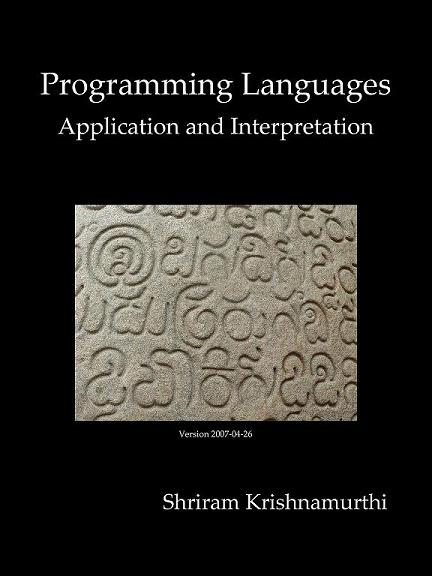
\includegraphics[height=\textheight]{lic/cover.jpg}&
\begin{minipage}{0.6\textwidth}
{\Large Programming Languages:\\Application and Interpretation}

\bigskip

{\small Copyright \copyright\ 2003-07, Shriram Krishnamurthi}

\bigskip

{\small Creative Commons\\Attribution-NonCommercial-ShareAlike 3.0\\United
States License}

\bigskip

{\small Original Version
\href{https://cs.brown.edu/~sk/Publications/Books/ProgLangs/2007-04-26/}{2007-04-26}}

{\small Warning: this translation was not confirmed\\by original author
\ref{krishna}}

\vspace{0.2cm}
{\tiny перевод Dmitry Ponyatov \email{dponyatov@gmail.com}\\\today}
\vspace{6cm}
\end{minipage}\\
\end{tabular}
\end{titlepage}
\tableofcontents
\secdown

\secrel{Introduction \ru{Введение}}\secdown
\clearpage
\secrel{Our Philosophy \ru{Наша философия}}

Please watch the video on \ru{Пожалуйста посмотрите это видео на}
\href{https://www.youtube.com/watch?v=3N__tvmZrzc}{YouTube}.

Someday there will be a textual description here instead.
\ru{Когда нибудь здесь будет полное текстовое описание того, о чем в нем
говориться.}

\secrel{The Structure of This Book\\\ru{Структура книги}}

Unlike some other textbooks, this one does not follow a top-down narrative.
\ru{В отличие от большинства учебников, эта книга не следует подходу ``сверху
вниз''.}
Rather it has the flow of a conversation, with backtracking.
\ru{Скорее она имеет форму повествования с возвратами к предыдущим темам.}
We will often build up programs incrementally, just as a pair of programmers
would.
\ru{Мы часто будет строить программы инкрементно, так же как мы бы это делали в
парном программировании.}
We will include mistakes,
\ru{Наш код будет включать ошибки,}
not because I don’t know the answer,
\ru{не потому что мы не знаем правильный ответ,}
but because \emph{this is the best way for you to learn.}
\ru{но потому что \emph{это лучший способ научить вас.}}
Including mistakes makes it impossible for you to read passively:
\ru{Включение намеренных ошибок делает невозможным для вас читать материал
пассивно:}
you must instead engage with the material,
\ru{вы должны взаимодействовать с ним,}
because you can never be sure of the veracity of what you’re reading.
\ru{потому что вы никогда не можете быть уверены в правильности того что вы
читаете.}

At the end, you’ll always get to the right answer.
\ru{В конце концов вы всегда получите правильный ответ.}
However, this non-linear path is more frustrating in the short term
\ru{Тем не меннее, это нелинейное повествование немного раздражающе в
краткосрочной перспективе}
(you will often be tempted to say,
\ru{у вас всегда будет соблазн сказать}
"Just tell me the answer, already\,!
\ru{Скажите же мне наконец ответ\,!}"),
and it makes the book a poor reference guide
\ru{и это также делает эту книгу плохим справочником}
(you can’t open up to a random page and be sure what it says is correct
\ru{вы не можете открыть произвольную страницу и быть уверенным что на ней
написана правда}).
However, that feeling of frustration is the sensation of learning.
\ru{Тем не менее, это чувство разочарования\ --- ощущение обучения.}
I don’t know of a way around it.
\ru{Я не знаю другого способа.}

\bigskip
At various points you will encounter this:
\ru{В некоторых местах вы встретите следующие выделения:}

\Exercise{
This is an exercise. Do try it.\\
\ru{Это упражнение. Попробуйте это сделать.}
}

This is a traditional textbook exercise.
\ru{Это традиционное для учебников упражнение.}
It’s something you need to do on your own.
\ru{Это то, что вам нужно сделать по своему усмотрению.}
If you’re using this book as part of a course,
\ru{Если вы используете эту книгу как часть курса,}
this may very well have been assigned as homework.
\ru{это упражнение хорошо задавать как домашнюю работу.}
In contrast, you will also find exercise-like questions that look like this:
\ru{В противоположность этому вы также можете найти подобные вопросы, выделенные
как}

\DoNow{
There’s an activity here\,! Do you see it\,?\\
\ru{Здесь предполагаются немедленные действия\,! Вы видите это\,?}
}

When you get to one of these, \emph{stop}.
\ru{Когда вы доберетесь до одного из этих блоков, \emph{остановитесь}.}
Read, think, and formulate an answer before you proceed.
\ru{Прочитайте, подумайте, сформулируйте ответ перед тем как продолжить чтение.}
You must do this because this is actually an \emph{exercise},
\ru{Вы должны сделать это потому что это действительно \emph{упражнение},}
but the answer is already in the book
\ru{но ответ уже есть в книге}\ ---
most often in the text immediately following
\ru{чаще всего в тексте непосредственно после упражнения}
(i.e., in the part you’re reading right now
\ru{т.е. в части которую вы сейчас читаете})\ ---
or is something you can determine for yourself by running a program.
\ru{или это что-то, что вы можете получить самостоятельно, запустив программу.}
If you just read on,
\ru{Если вы просто продолжите читать,}
you’ll see the answer without having thought about it
\ru{то вы увидете ответ без его обдумывания}
(or not see it at all, if the instructions are to run a program
\ru{или не увидите его вообще, если это инструкции по запуску программы}),
so you will get to neither
\ru{так что вы ни}
(a) test your knowledge, nor \ru{проверите свои знания, ни}
(b) improve your intuitions. \ru{улучшите свое понимание.}
In other words, these are additional, explicit attempts to encourage active
learning.
\ru{Другими словами, это дополнительные, явные попытки стимулировать ваше
активное обучение.}
Ultimately, however, I can only encourage it;
\ru{В конце концов, я могу только поощрять вас работать;}
it’s up to you to practice it.
\ru{решение применять это или нет остается за вами.}

\secrel{The Language of This Book\\\ru{Язык программирования используемый в
книге}}

The main programming language used in this book is
\ru{Язык программирования используемый в книге}\ --- 
\href{http://www.racket-lang.org/}{\racket}.
Like with all operating systems, however,
\ru{Аналогично операционным системам,}
\racket\ actually supports a host of programming languages,
\ru{\racket-система является исполняющей средой для целого ряда языков
программирования,}
so you must tell \racket\
\ru{так что вы должны указать \racket у}
\emph{which} language you’re programming in.
\ru{\emph{на каком} языке вы программируете.}
You inform the Unix shell by writing a line like
\ru{Например, в Unix вы пишете строку типа}

\begin{verbatim}
#!/bin/sh
\end{verbatim}
at the top of a script;
\ru{в первой строке shell-скрипта;}
you inform the browser by writing, say,
\ru{вы указываете веб-браузеру тип документа, добавляя заголовок}

\begin{verbatim}
<!DOCTYPE HTML PUBLIC "-//W3C//DTD HTML 4.01//EN" ...>
\end{verbatim}

Similarly, \racket\ asks that you declare which language you will be using.
\ru{Аналогично, \racket\ требует от вас указать какой язык вы будете
использовать.}
\racket\ languages can have the same parenthetical syntax as \racket\ but with a
different semantics;
\ru{Диалекты языков \racket\ имеют тот же скобочный синтаксис, что и сам
\racket, но другую семантику;}
the same semantics but a different syntax;
\ru{ту же семантику но другой синтаксис;}
or different syntax and semantics.
\ru{или различные синтаксис и семантику.}
Thus every \racket\ program
\ru{Так что каждая программа, которую может выполнять \racket-система,}
begins with \#lang followed by the name of some language:
\ru{начинается со строки \#lang за которой следует имя диалекта языка:}
by default, it’s \racket\ \ru{по умолчанию, это оригинальный \racket\ }
written as \ru{указыватся как} \verb|racket|).
In this book we’ll almost always use the language\note{In DrRacket v.5.3,
go to\\
Language, then Choose Language, and select ``Use the language declared in
the source''.}
\ru{В этой книге мы почти всегда будем использовать диалект}\note{\ru{В DrRacket
v.6.6, выберите меню\\\menu{Язык > Выбрать язык\ldots > Start your program with
\#lang to specify the desired dialect}.}}
\begin{verbatim}
#lang plai-typed
\end{verbatim}
When we deviate we’ll say so explicitly,
\ru{Когда мы будем отклоняться от этого правила, это будет указано особо,}
so unless indicated otherwise, put
\ru{так что если не указано иное, добавляйте заголовок}
\verb|#lang plai-typed|
at the top of every file
\ru{в начало каждого файла программы}
(and assume I’ve done the same
\ru{предполагается что я тоже это
сделал})\note{В DrRacket v.6.6 требуется установить расширение
plai-typed:\\\menu{Файл>Install package\ldots>Package
Source:>\url{github://github.com/mflatt/plai-typed/master}>Install>\ldots>Закрыть}}.

The \termdef{Typed PLAI}{Typed PLAI}\ language differs from traditional \racket\
most importantly by being statically typed.
\ru{Язык \term{Typed PLAI}\ отличается от традиционного \racket\ в основном
\emph{статической типизацией}.}
It also gives you some useful new constructs:
\ru{Он также дает вам некоторые новые полезные конструкции:}
\verb|define-type| \ru{определение-типа}, \verb|type-case| \ru{выбор-по-типу},
and \verb|test|\note{There are additional commands for controlling the output
of testing, for instance. \ru{Также существуют дополнительные команды для
управления выводом тестов.} Be sure to read the documentation for the language.
\ru{Обязательно прочитайте документацию для языка.}
In DrRacket v.5.3, go to \menu{Help>Help Desk}, and in the Help Desk search bar,
type \menu{plai-typed}. \ru{В DrRacket v.6.6 идите в меню \menu{Help>Help
Desk>plai-typed}.}}
Here’s an example of each in use.
\ru{Вот примеры использования каждого из них.} 
We can introduce new datatypes
\ru{Мы можем создавать новые типы данных\note{запустить программу можно нажав
\keys{Ctrl+R}}}:
\lst{1/3/p8_1.rkt}
You can roughly think of this as analogous to the following in Java:
\ru{Вы можете примерно понять идею в терминах языка \java:}
an abstract class \term{абстрактный класс} \verb|MisspelledAnimal| and two
concrete sub-classes \ru{и два конкретизирующих подкласса}\ \verb|caml|
\ru{верблд} and \verb|yacc| \ru{якк},
each of which has one numeric constructor argument named
\ru{каждый из которых имеет конструктор с числовым аргументом}
\verb|humps| \ru{горбы} and \verb|height| \ru{высота}, respectively
\ru{соответственно}.

In this language, we construct instances as follows:
\ru{На этом языке мы строим экземпляры классов следующим
образом:\note{выполните это \emph{в командной строке \racket}, и посмотрите на
класс результата}}
\lst{1/3/p8_2.rkt}
As the name suggests, \ru{Как следует из названия,} \verb|define-type| creates
a type of the given name \ru{создает тип с заданным именем}.
We can use
this when, for instance, binding the above instances to names:
\ru{Мы можем это использовать например при связывании экземпляров с именами:}
\lst{1/3/p8_3.rkt}
In fact you don’t need these particular type declarations,
\ru{Фактически вам не нужны эти частные определения типов,} 
because \term{Typed PLAI} will infer types for you here and in many other cases.
\ru{так как \term{Typed PLAI} в этом и других случаях будет сам делать для вас
\term{вывод типов}.}
Thus you could just as well have written
\ru{Так что вы можете написать короче}
\lst{1/3/p8_4.rkt}
but we prefer to write explicit type declarations
\ru{но мы предпочтем писать полные объявления типов}
as a matter of both discipline and comprehensibility when we return to programs
later.
\ru{с точки зрения как
дисциплины, так и усвояемости, когда мы вернемся к программам позже.}

The type names can even be used recursively, as we will see repeatedly in this
book (for instance, section \ref{sec2_4}).
\ru{Имена типов даже могут быть использованы рекурсивно, как мы увидим
несколько позже в этой книге (например в разделе \ref{sec2_4}).}

The language provides a pattern-matcher for use when writing expressions, such
as a function’s body:
\ru{Язык предоставляет pattern-matcher для использования при написании
выражений, таких как тело функции:}
\lst{1/3/p9_1.rkt}
In the expression \ru{Например в выражении} (>= humps 2), for instance,
\verb|humps| is the name given to whatever value was given as the argument to
the constructor \ru{имя humps соответствует любому значению, данному как
аргумент для конструктора} \verb|caml|.

Finally, you should write test cases, ideally before you’ve defined your
function, but also afterwards to protect against accidental changes:
\ru{И наконец, вы должны написать тесты, в идеале до того как вы ее реализовали,
или хотя бы после, чтобы защититься от внезапных несоответствий в ее поведении
при внесении изменений в код:}
\lst{1/3/p9_2.rkt}
When you run the above program, the language will give you verbose output telling
you both tests passed.
\ru{При запуске тестов язык даст вам подробный отчет, что оба теста успешно
пройдены.}
Read the documentation to learn how to suppress most of these messages.
\ru{Прочитайте документацию, чтобы узнать как подавить вывод большей части
этих сообщений.}

Here’s something important that is obscured above.
\ru{Вот еще кое-что важное, что было неясно выше.}
We’ve used the same name,
\ru{Мы использовали одно и то же имя,}
humps (and height), in \emph{both} the datatype definition and in the fields of
the patternmatch.
\ru{и в определении типа данных, и в полях объекта при проверке совпадения
шаблонов.}
This is absolutely unnecessary because the two are related by \emph{position},
not name.
\ru{Это совершенно необязательно, так как каждая пара связана по \emph{позиции},
а не по имени.}
Thus, we could have as well written the function as
\ru{Так что мы могли бы также написать эту функцию как}
\lst{1/3/p9_3.rkt}
Because each $h$ is only visible in the case branch in which it is introduced,
the two $h$s do not in fact clash.
\ru{Так как каждый $h$ виден только в той case-секции, где он используется,
два $h$ фактически не сталкиваются.}
You can therefore use convention and readability to
dictate your choices.
\ru{Таким образом вы можете использовать соглашения по оформлению кода для
улучшения читаемости, и диктовать свой выбор.}
In general, it makes sense to provide a long and descriptive name
\ru{В общем, имеет смысл использовать длинные описательные имена}
when defining the datatype\note{because you probably won’t use
that name again},
\ru{при определении типа данных\note{\ru{потому что вы возможно больше никогда
не будете использовать это имя снова}},}
but shorter names in the \class{type-case} because you’re likely to use use
those names one or more times.
\ru{и короткие имена в \class{type-case}, где они обычно используются несколько
раз.}

I did just say you’re unlikely to use the field descriptors introduced in the
datatype definition, but you can.
\ru{Также я хочу упомянуть декрипторы полей класса, которые вы возможно
захотите использовать.}
The language provides \term{selectors} to extract fields without the need for
pattern-matching: e.g., \class{caml-humps}.
\ru{Язык предоставляет \term{селекторы} для получения значений полей без
необходимости использовать pattern-matching, например \class{caml-humps}.}
Sometimes,
it’s much easier to use the selector directly rather than go through the
pattern-matcher.
\ru{Иногда намного проще использовать селектор, чем возиться с мэтчингом
шаблонов.}
It often isn’t, as when defining \class{good?}\ above,
\ru{Часто это не так, как в случае определения \class{good?},}
but just to be clear, let’s write it without pattern-matching:
\ru{но для ясности давайте напишем без pattern-matching:}
\lst{1/3/p9_4.rkt}

\DoNow{
What happens if you mis-apply functions to the wrong kinds of values\,?\\
\ru{Что произойдет, если вы ошибочно примените функции к неправильным типам
значений\,?}

For instance, what if you give the \class{caml}\ constructor a string\,?\\
\ru{Например, что если вы дадите конструктору \class{caml}\ строковый
аргумент\,?}

What if you send a number into each version of \class{good?}\ above\,?\\
\ru{Что произойдет если вы пошлете число к каждой версии \class{good?}\
описанных выше\,?} }

\secdown\secrel{\ru{Реализация динамического языка на \cpp}}

Параллельно с основным текстом оригинальной книги были добавлены разделы по
реализации динамического языка на паре mainstream языков; прежде всего это
комплект flex/bison/\cpp.

Диалект \lisp а, использованный в книге, хорош для описания логики. Но для
практического применения больше подходит реализация в виде
\termdef{встраиваемого интерпретатора}{встраиваемый интерпретатор}\ --- вы
можете взять свою готовую программу, и добавить в нее скриптовый движок,
расширяющий возможности (расширение пользователем, реализация языковых фич
недоступных в \cpp, сборка мусора,\ldots). $DrRacket$ слишком тяжел по ресурсам
для встраивания, и хотелось бы иметь образец реализации на более низкоуровневом
языке.

\bigskip

Показаны реализации двух языков:
\begin{enumerate}[nosep]
  \item \bi\ питоно-подобный инфиксный язык для быстрого напиcания скриптов в
  привычном синтаксисе, и
  \item \hm\ экспериментальный гомоиконичный язык для
  мета-про\-грам\-ми\-ро\-ва\-ния.
\end{enumerate}

\secup

\secup

\secrel{Everything (We Will Say) About Parsing\\
\ru{Все (что мы будем говорить) о разборе}}\label{allparsing}\secdown

Parsing is the act of turning an input character stream into a more structured,
internal representation.
\ru{\termdef{Парсинг}{парсинг} или \termdef{разбор}{синтаксический разбор}\
--- процесс превращения входного потока одиночных символов в более
структурированное внутреннее представление\note{программы или данных, заданных в
текстовой синтаксической форме}.}
A common internal representation is as a tree, which programs can recursively
process.
\ru{Обычно используется внутреннее представление в виде дерева, которое может
быть обработано программой рекурсивно.}

For instance, given the stream
\ru{Например, для входного потока символов\note{включая пробелы, табуляции и
концы строк}}
\begin{verbatim}
23 + 5 - 6
\end{verbatim}
we might want a tree representing addition whose left (L) node represents the
number 23 and whose right (R) node represents subtraction of 6 from 5.
\ru{мы хотим получить деревянное представление сложения, в котором левая (L)
ветвь содержит число 23, а правая (R)\ --- вложенное представление вычитания 6
из 5.}
A parser is responsible for performing this transformation.
\ru{Парсер отвечает за выполнение такой транформации.}

\noindent
\begin{tabular}{c c}
\noindent\includegraphics[height=0.8\textheight]{tmp/2_p10_R.pdf}
&
\noindent\includegraphics[height=0.8\textheight]{tmp/2_p10_L.pdf}
\\
\emph{Право}ассоциативный разбор
&
(*) \emph{Лево}ассоциативный разбор
\\
\end{tabular}\bigskip

Parsing is a large, complex problem that is far from solved due to the
difficulties of ambiguity.
\ru{Парсинг\ --- большая проблема информатики, сложность которой
заключается в трудностях неоднозначности.}
For instance, an alternate parse tree (*) for the above input expression might
put subtraction at the top and addition below it.
\ru{Например, существует альтернативное (*) \termdef{дерево разбора}{дерево
разбора} для того же входного выражения, в котором мы можем поместить
вычитание на вершину дерева, а сложение будет вложенным поддеревом.}
We might also want to consider
\ru{Нас также может интересовать,}
whether this addition operation is commutative
\ru{является ли это сложение коммутативной операцией,}
and hence whether the order of arguments can be switched.
\ru{то есть можем ли мы изменить порядок аргументов\note{например для
оптимизации кода}.}
Everything only gets much, much worse when we get to full-fledged programming
languages (to say nothing of natural languages).
\ru{Все становится намного хуже для полноценных языков программирования
(не говоря о натуральных языках).}

\secrel{A Lightweight, Built-In First Half of a Parser
\ru{Легковесная встроенная часть парсера}}

These problems make parsing a worthy topic in its own right, and entire books,
tools, and courses are devoted to it.
\ru{Эти проблемы делают разбор достойной темой саму по себе, и ей посвящены
целые книги, утилиты и учебные курсы, например первая глава ``Книги Дракона''
\cite{dragon}.}
However, from our perspective parsing is mostly a distraction, because we want
to study the parts of programming languages that are not parsing.
\ru{Однако, с нашей точки зрения тема парсинга является сильным отвлечением,
так как есть другие более достойные темы, касающиеся реализации языков
программирования.}
We will therefore exploit a handy feature of \racket\ to manage the
transformation of input streams into trees: 
\ru{Поэтому мы сделаем финт ушами, и будем использовать встроенную фичу
\racket а для получения готовых деревьев разбора из входного потока: функцию}
\verb|read|.
\verb|read| is tied to the parenthetical form of the language, in that it parses
fully (and hence unambiguously) parenthesized terms into a built-in tree form.
\verb|read| \ru{привязана к скобочной форме языка, и полностью (и следовательно
однозначно) разбирает скобочные выражения во встроенное представление\ ---
дерево.}
For instance, running \ru{Например применение} \verb|(read)| on the
parenthesized form of the above input \ru{к следующему входному потоку символов
(включающему скобки)}\ ---
\begin{verbatim}
(+ 23 (- 5 6))
\end{verbatim}
--- will produce a list, whose first element is the symbol \ru{создаст список, в
котором первым элементом будет символ} \verb|'+|, second element is the number
\ru{вторым элементом число} 23, and third element is a list \ru{и третий
элемент список}: this list’s first element is the
symbol \ru{в котором первым элемент будет} \verb|'-|, second element is the
number \ru{второй элемент число} 5, and third element is the number \ru{и
третий элемент число} 6.

\fig{\ru{Дерево разбора для} (+ 23 (- 5 6))}{tmp/2_1.pdf}{height=0.9\textheight}

\lst{2/p10_1.rkt}

\secrel{A Convenient Shortcut \ru{Удобный трюк}}

As you know you need to test your programs extensively, which is hard to do when you
must manually type terms in over and over again.
\ru{Как вы знаете, нужно тщательно тестировать свои программы, что особенно
сложно, если вам нужно снова и снова вводить выражения вручную.}
Fortunately, as you might expect, the parenthetical syntax is integrated deeply
into \racket\ through the mechanism of quotation.
\ru{К счатью, как и следовало ожидать, скобочный синтаксис глубоко
интегрирован в \racket\ через механизм \termdef{квотирования}{квотирование}.}
That is, \ru{это то самое выражение} \verb|'<expr>|\ --—
which you saw a moment ago in the above example
\ru{которое вы видели только что при выполнении предыдущего примера}\ --- 
acts as if you had run \ru{действует так же, как если бы вы запустили}
\verb|(read)| and typed \ru{и ввели} <expr> at the prompt \ru{в текстовом поле
ввода} (and, of course, evaluates to the value the (read) would have
\ru{и конечно же вычисляется в то же значение, что дает} \verb|(read)|).

\secrel{Types for Parsing \ru{Типы для разбора}}

Actually, I’ve lied a little.
\ru{На самом деле, я немного соврал.}
I said that \ru{я сказал что} \verb|(read)|\ --- or equivalently, using
quotation \ru{или использование квотирования, что эквивалентно}\ --- will
produce a \emph{list}, etc. \ru{создаст \emph{список}, блаблабла.}
That’s true in regular \racket, but in $Typed PLAI$
\ru{Это так для оригинального \racket, но в $Typed PLAI$} the type it
returns a distinct type called an \ru{возвращается специальный тип, который
называется} \termdef{s-expression}{s-expression}
\ru{s-выражение\index{s-выражение}}, written in $Typed PLAI$ as
\ru{который в $Typed PLAI$ записывается как}
\verb|s-expression|:
\begin{verbatim}
> (read)
- s-expression
[type in (+ 23 (- 5 6))]
'(+ 23 (- 5 6))
\end{verbatim}
\racket\ has a very rich language of s-expressions
\ru{имеет очень богатый язык на s-выражениях}
(it even has notation to represent cyclic structures
\ru{он даже имеет нотацию для представления циклических структур}), 
but we will use only the simple fragment of it.
\ru{но мы будем использовать только простейшую часть этого синтаксиса.}

In the typed language, an s-expression is treated distinctly from the other
types, such as numbers and lists.
\ru{В типизированном языке s-выражения обрабатыватся обособленно от других
типов, таких как числа и списки.}
\begin{framed}
Underneath, an s-expression is a large
recursive datatype that consists of all the base printable values—numbers,
strings, symbols, and so on—and printable collections (lists, vectors, etc.) of
s-expressions.
\ru{Далее s-выражение рассматривается как большой рекурсивный тип данных,
который содержит все базовые отображаемые (представимые в тексте) значения\
--- числа, строки, символы и т.д.\ --- и коллекции (списки, вектора и т.д.)
других s-выражений}.
\end{framed}
As a result, base types like numbers, symbols, and strings are
\emph{both} their own type and an instance of s-expression.
\ru{В результате такие базовые типы как числа, символы и строки, могут
\emph{одновременно} являться как собственным типом (число,..), так и
экземпляром s-выражениея}.
Typing such data can be fairly problematic, as we will discuss later
\ru{Типизация таких данных может быть очень проблематична, детальнее мы обсудим
это позже} \ref{}.

$Typed PLAI$ takes a simple approach.
\ru{$Typed PLAI$ применяет более простой подход.}
When written on their own, values like numbers are of those respective types.
\ru{Когда значания простых типов, типа чисел, написаны сами по себе, они
являются собственными типами (число).}
But when written inside a complex
s-expression—in particular, as created by read or quotation—they have type
s-expression.
\ru{Но когда они включены в состав сложного s-выражения\ --- в частности,
созданы через (read) или квотацию\ --- они имеют тип s-выражения.}
You have to then cast them to their native types.
\ru{Вы должны привести их к нативному типу.}
For instance \ru{Например}:
\lstl{2/p11_1.rkt}
This is similar to the casting that a Java programmer would have to insert.
\ru{Это похоже на явное приведение типов, которое должен вставить программист
на \java.}
We will study casting itself later \ru{Мы обсудим само приведение типов позже}
\ref{}.

Observe that the first element of the list is still not treated by the
type checker as a symbol:
\ru{Отметим, что первый элемент списка все еще не распознается контролером
типов как символ:}
a list-shaped s-expression is a list of s-expressions.
\ru{списко-образное s-выражение является списком s-выражений.}
Thus \ru{Таким образом},
\lst{2/p11_2.rkt}
whereas again, casting does the trick:
\ru{и снова приведение типов решает проблему :}
\lst{2/p11_3.rkt}
The need to cast s-expressions is a bit of a nuisance,
\ru{Необходимость приведения s-выражений немного геморна,}
but some complexity is unavoidable because of what we’re trying to accomplish:
\ru{но некоторая сложность неизбежна из-за того что мы пытаемся достичь:}
to convert an \emph{untyped input} stream into a \emph{typed output} stream
\ru{преобразование \emph{нетипизированного} входного потока в
\emph{типизированный} выходной поток}
through robustly typed means.
\ru{через средства робастной типизации.}
Somehow we have to make explicit our assumptions about that input stream.
\ru{Каким-то образом мы должны делать явные предположения об этом входном
потоке.}

Fortunately we will use s-expressions only in our parser, and our goal is to
\emph{get away from parsing as quickly as possible\,!}
\ru{К счастью, мы будем использовать s-выражения только в нашем парсере, и наша
цель состоит в том, чтобы \emph{уйти от разбора как можно быстрее\,!}}
Indeed, if anything this should be inducement to get away even quicker.
\ru{В самом деле, все эти заморочки являются побуждением сделать этот уход еще
быстрее.}

\secrel{Completing the Parser\\
\ru{Заканчиваем с парсером}}\label{sec2_4}

In principle, we can think of \ru{В принципе, мы можем думать о} \verb|read|\
as a complete parser \ru{как о законченном парсере}.
However, its output is generic \ru{Тем не менее, его вывод все еще сырой}:
it represents the token structure without offering any comment on its intent.
\ru{он содержит структуру токенов не предлагая каких-либо комментариев об их
назначении.}
We would instead prefer to have a representation
\ru{Вместо этого мы предпочли бы иметь представление,}
that tells us something about the \emph{intended meaning} of the terms in our
language,
\ru{которое говорит нам что-то о \emph{предполагаемом значении} термов нашего
языка,}
just as we wrote at the very beginning: “representing addition”, “represents a
number”, and so on.
\ru{так же как мы писали в самом начале: ``представление сложения'',
``представление числа'' и так далее.}

To do this, we must first introduce a datatype
\ru{Чтобы сделать это, мы сначала введем тип данных,}
that captures this representation.
\ru{который зафиксирует это представление.}
We will separately discuss \ru{Мы
отдельно рассмотрим} (section \ru{в разделе} \ref{sec31}) how and why we obtained this
datatype \ru{как и зачем мы применяем этот тип}, but for now let’s say it’s
given to us \ru{но сейчас пока будем считать, что он нам задан}:
\lstx{ArithC.rkt}{2/p12_1.rkt}{rkt}\label{arithc}
We now need a function that will convert s-expressions into instances of this
datatype.
\ru{Теперь нам нужна функция, которая преобразует s-выражение в структуру из
экземпляров этого типа.}
This is the other half of our parser \ru{Это вторая половина нашего парсера}:
\lstxl{ArithC.rkt}{2/p12_2.rkt}{rkt}

Thus\note{typing in \racket\ console \emph{after program run}} \ru{Таким
образом\note{\ru{введя выражение в \racket-консоли \emph{после выполнения
программы}}}}
\lst{2/v1.rkt}
\lstx{ArithC.rkt}{2/p12_3.rkt}{rkt}
\lst{2/v2.rkt}

Congratulations\,! \ru{Мои поздравления\,!}
You have just completed your first representation of a program.
\ru{Вы только что завершили ваше первое представление программы.}
From now on we can focus entirely on programs
\ru{С этого момента мы можем полностью сосредоточиться на программах,}
represented as recursive trees,
\ru{представленных в виде рекурсивных деревьев,}
ignoring the vagaries of surface syntax
\ru{не обращая внимания на капризы наносного синтаксиса}
and how to get them into the tree form.
\ru{и процесс получения из него дерева разбора.}
We’re finally ready to start studying programming languages\,!
\ru{Мы, наконец, готовы приступить к изучению языков программирования\,!}

\Exercise{
What happens if you forget to quote the argument to the 
\ru{Что случиться, если вы забудете заквотить аргумент вызова}
parser\,?
Why\,? \ru{Почему\,?}
}
\secrel{Coda \ru{Кода}}

\racket’s syntax, which it inherits from Scheme and \lisp, is controversial.
\ru{Синтаксис \racket а, который он наследует от Scheme и Lisp, спорен.}
Observe, however, something deeply valuable that we get from it.
\ru{Заметим, однако, что мы получаем от него нечто глубоко ценное.} 
While parsing traditional languages can be very complex,
\ru{В то время как парсинг традиционных языков может быть очень сложным,}
parsing this syntax is virtually trivial.
\ru{разбор этого синтаксиса практически тривиален.}
Given a sequence of tokens corresponding to the input,
\ru{Для заданной последовательности лексем, соответствующих входному потоку,}
it is absolutely straightforward to turn paren\-the\-sized sequences into
s-expressions;
\ru{абсолютно тривиально превратить скобочные последовательности в s-выражения;}
it is equally straightforward (as we see above) to turn sexpressions into proper
syntax trees.
\ru{столь же просто (как мы видим выше) преобразовать s-выражения в правильные
синтаксические деревья.}
I like to call such two-level languages \term{bicameral}, in loose analogy to
government legislative houses:
\ru{Мне нравится называть такие двухуровневые языки \term{двухпалатными}, в
свободной аналогии к государственным законодательным учреждениям:}
the lower-level does rudimentary well-formedness checking, while the upper-level
does deeper validity checking.
\ru{нижний уровень делает рудиментарную проверку правильности оформления, в то
время как верхний уровень выполняет глубокую проверку валидности.}
(We haven’t done any of the latter yet, but we will
\ru{Мы еще не делали последнего, но мы будем}
\ref{}.)

The virtues of this syntax are thus manifold.
\ru{Достоинства этого синтаксиса, таким образом, многообразны.}
The amount of code it requires is small, and can easily be embedded in many
contexts.
\ru{Объем кода, который он требует, очень мал, и может быть встроен во многих
контекстах.}
By integrating the syntax into the language, it becomes easy for programs to
manipulate representations of programs (as we will see more of in \ref{}).
\ru{Интеграция синтаксиса в язык делает простой программную манипуляцию
представлением программ (как мы увидим в \ref{}).}
It’s therefore no surprise that even though many Lisp-based syntaxes have had
wildly different semantics, they all share this syntactic legacy.
\ru{Поэтому неудивительно, что множество основанных на \lisp е синтаксисов,
имеющих дико разную семантику, все равно разделяют это общее синтаксическое
наследие.}

Of course, we could just use XML instead.
\ru{Конечно, мы могли бы использовать XML.}
That would be much better.
\ru{Это было бы намного лучше.}
Or JSON.
\ru{Или JSON.}
Because that wouldn’t be anything like an s-expression at all.
\ru{Потому что все равно это в итоге было бы тем же s-выражением.}

\secup

\secrel{A First Look at Interpretation \ru{Первый взгляд на
интерпретацию}}\label{firstinterp}\secdown

Now that we have a representation of programs, there are many ways in which we
might want to manipulate them.
\ru{Теперь, когда мы имеем представление программ, существует множество
способов, которыми мы можем манипулировать ими.}
We might want to display a
program in an attractive way \ru{Мы можем захотеть выводить листинг программы в
красивом виде} (“pretty-print”), convert into code in some other format
\ru{преобразовать в код в какой-то другой формат} (“compilation”
\ru{``компиляция''/''трансляция''}), ask whether it obeys certain properties 
\ru{убедиться что она отвечает определенным требованиям}
(“verification” \ru{``верификация''}), and so on \ru{и так далее}.
For now, we’re going to focus on asking what value it corresponds to
(“\termdef{e\underline{val}uation}{evaluation}”\ --- the reduction of programs
to \emph{\underline{val}ues}).
\ru{Для начала, мы собираемся сфокусироваться на вопросе\ --- какому значению
соответствует программа (“\termdef{вычисление}{вычисление}"\ --- редукция
программы до \emph{значения})}

Let’s write an evaluator, in the form of an \termdef{interpreter}{interpreter},
for our arithmetic language.
\ru{Давайте напишем вычислитель, в форме
\termdef{интерпретатора}{интерпретатор}, для нашего арифметического языка.}
We choose arithmetic first for three reasons \ru{Мы выбрали арифметику прежде
всего по следующим трем причинам}:
\begin{itemize}[nosep]
  \item[(a)]
  you already know how it works, so we can focus on the mechanics of writing
evaluators;
\ru{вы уже знаете как работает арифметика, и мы можем сфокусироваться на
механике написания вычислителей;}
  \item[(b)]
  it’s contained in
every language we will encounter later, so we can build upwards and outwards from it;
\ru{она содержится в каждом языке, с которым мы столкнемся в дальнейшем, так
что мы будем расширять этот арифметический язык вверх и вширь;} and \ru{и}
  \item[(c)] 
it’s at once both small and big enough to illustrate many points
we’d like to get across.
\ru{этот язык минималистичен, но при этом достаточно большой, чтобы
проиллюстрировать многие моменты, которые мы хочем до вас донести.}
\end{itemize}

\secrel{Representing Arithmetic\\
\ru{Представление арифметики}}\label{sec31}

Let’s first agree on how we will represent arithmetic expressions.
\ru{Давайте сначала договориться о том, как мы будем представлять арифметические
выражения.}
Let’s say we want to support only two operations\ --- addition and
multiplication\ --- in addition to primitive numbers.
\ru{Допустим, мы хотим поддерживать только две простые операции\ --- сложение и
умножение\ --- в дополнение к примитивным числам.}
We need to represent arithmetic \termdef{expressions}{expression}.
\ru{Нам необходимо представление для арифметических
\termdef{выражений}{выражение}}.
What are the rules that govern nesting of arithmetic expressions\,?
\ru{Какие правила регулируют вложенность арифметических выражений\,?} 
We’re actually free to nest any expression inside another.
\ru{На самом мы свободно можем владывать любое выражение внутрь любого другого.}

\DoNow{
Why did we not include division\,?
\ru{Почему мы не включили деление\,?}
\\
What impact does it have on the remarks above\,?
\ru{Какое влияние это имеет на замечания выше\,?}
}

We’ve ignored division
\ru{Мы игнорировали деление,}
because it forces us into a discussion of what
expressions we might consider legal:
\ru{потому что оно вовлекает нас в дикуссию о том,
какие выражения мы можем считать правильными:}
clearly the representation of $1/2$ ought to be legal;
\ru{ясно что представление $1/2$ должно быть легальным;} 
the representation of $1/0$ is much more debatable;
\ru{представление $1/0$ спорно;}
and that of \ru{и что-то типа} $1/(1-1)$ seems even more controversial.
\ru{кажется гораздо более противоречивым.}
 
We’d like to sidestep this controversy for now and return to it later
\ru{Мы хотели бы обойти сейчас это противоречие, в вернуться к нему позже}
\ref{}.

Thus, we want a representation for numbers and arbitrarily nestable
addition and multiplication.
\ru{Таким образом нам нужно представление для чисел и произвольно вложенных
сложений и умножений.} 
Here’s one we can use \ru{Вот то что мы можем использовать}
(used in \ru{использовано в} \ref{arithc} ):
\lstx{ArithC}{2/p12_1.rkt}{rkt}

\secrel{Writing an Interpreter \ru{Написание интерпретатора}}

Now let’s write an interpreter for this arithmetic language.
\ru{Теперь давайте напишем интерпретатор для этого арифметического языка.} 
First, we should think about what its type is.
\ru{Для начала нам надо подумать, какие типы он использует\,?} 
It clearly consumes a \verb|ArithC| value.
\ru{Совершенно ясно что на вход подается структура типа} \verb|ArithC|. 
What does it produce\,?
\ru{Что он возвращает\,?} 
Well, an interpreter evaluates
\ru{Ну, интерпретатор вычисляет} \ --- and what kind of value might arithmetic
expressions reduce to\,?
\ru{и к какому значению может редуцироваться арифметическое выражение\,?} 
Numbers, of course.
\ru{Конечно, числу.} 
So the interpreter is going to be a function from arithmetic expressions to
numbers.
\ru{Таким образом, интерпретатор должен быть функцией от арифметического
выражения, возвращающей число.}

\Exercise{
Write your test cases for the interpreter.
\ru{Напишите тесты для интерпретатора.}
}

Because we have a recursive datatype, it is natural to structure our interpreter
as a recursive function over it.
\ru{Так как мы имеем рекурсивный тип данных\note{допускаются произвольные
вложения того же типа}, нормально что структура нашего интерпретатора тоже
должна быть рекурсивной функций над выражением.}
Here’s a first template\note{Templates are
explained in great detail in \emph{How to Design Programs}.}
\ru{Вот первый шаблон\note{\ru{Шаблоны очень детально описаны в \emph{How to
Design Programs}}}} :
\lstx{ArithC.rkt}{3/p14_1.rkt}{rkt}
You’re probably tempted to jump straight to code, which you can:
\ru{Вероятно у вас есть соблазн сразу перейти к коду, который вы можете
написать:}
\lstx{ArithC.rkt}{3/p14_2.rkt}{rkt}

\DoNow{
Do you spot the errors\,?
\ru{Вы увидели ошибки\,?}
}

Instead, let’s expand the template out a step:
\ru{Вместо этого давайте расширим шаблон на один шаг:}
\lstx{ArithC.rkt}{3/p15_2.rkt}{rkt}
and now we can fill in the blanks:
\ru{и теперь мы можем заполнить пробелы:}
\lstx{ArithC.rkt}{3/p15_3.rkt}{rkt}

Later on \ru{Позже в} \ref{}, we’re going to wish we had returned a more complex
datatype than just numbers.
\ru{мы пожелаем возвращать более сложный тип данных, чем просто числа.}
But for now, this will do.
\ru{Но сейчас нам этого достаточно.}

Congratulations: you’ve written your first interpreter\,!
\ru{Поздравляем: вы только что написали свой первый интерпретатор\,!} 
I know, it’s very nearly an anticlimax\note{\ru{ситуация, когда проблема
казавшеяся очень сложной, решается с помощью чего-то тривиального //
Wikipedia}}\note{\ru{род морских улиток // там же}}.
\ru{Я знаю, это очень близко к разочарованию.}
But they’ll get harder\ --- much harder\ --- pretty soon, I promise.
\ru{Но все станет жестче\ --- намного жестче\ --- совсем скоро, я обещаю.}

\secrel{Did You Notice\,?\\
\ru{Вы заметили\,?}}

I just slipped something by you:
\ru{Я только что утаил что-то от вас:}
\DoNow{
What is the ``meaning'' of addition and multiplication in this new language\,?
\ru{Каков ``смысл'' сложения и умножения в этом новом языке\,?}
}

That’s a pretty abstract question, isn’t it.
\ru{Это достаточно абстрактный вопрос, не так ли.} 
Let’s make it concrete.
\ru{Давайте его конкретизируем.} 
There are many kinds of addition in computer science:
\ru{В информатике существует множество видов сложения:}

\begin{itemize}
  \item 
First of all, there’s many different kinds of \termdef{numbers}{number}:
\ru{Прежде всего, существует множество видов \termdef{чисел}{число}:}
fixed-width \ru{фиксированной длины} (e.g., 32- bit \ru{например 32-битные})
integers \ru{целые}, signed fixed-width \ru{знаковые фиксированной длины} (e.g.,
31-bits plus a sign-bit \ru{например 31-битные плюс бит знака}) integers
\ru{целые}, arbitrary precision integers \ru{целые числа произвольной точности};
in some languages, rationals \ru{в некоторых языках\ --- натуральные дроби};
various formats of fixed- and floating-point numbers
\ru{различные форматы чисел с фиксированной и плавающей точкой}; in some
languages, complex numbers \ru{в некоторых языках комплектные числа}; and so on
\ru{и так далее}.
After the numbers have been chosen, addition may support only some combinations
of them.
\ru{После того как были выбраны определенные виды чисел, сложение может
поддерживать только некоторые их комбинации.}
  \item 
In addition, some languages permit the addition of datatypes such as matrices.
\ru{В дополнение, некоторые языки поддерживают сложение таких типов данных, как
матрицы.}
  \item 
Furthermore, many languages support ``addition'' of strings
\ru{Кроме того, многие языки поддерживают ``сложение'' строк} (
we use scare-quotes because we don’t really mean the mathematical concept of
addition, but rather the operation performed by an operator with the syntax +
\ru{Мы используем кавычки, так как предполагаем не математическую идею
сложения, а операцию, выполняемую оператором с синтаксисом +} ). 
In some languages this always means concatenation;
\ru{В некоторых языках это всегда значит конкатенацию строк;} 
in some others, it can result in numeric results (or numbers stored in strings).
\ru{в некоторых долбанутых языках иногда может получиться численный
результат (или числа хранимые в строках).}
\end{itemize}

These are all different meanings for addition. 
\ru{Все это является смыслом сложения.}
\termdef{Semantics}{semantics}
is the mapping of \emph{syntax} (e.g., +) to \emph{meaning} (e.g., some or all
of the above).
\ru{\termdef{Семантика}{семантика} это отображение \emph{синтаксиса} (например
+) на \emph{смысл} (например что-то или все из вышеперечисленного).}

This brings us to our first game of:
\ru{Это подводит нас к первоначальной игре:}
\begin{description}\item[\emph{Which of these is the same\,?} \ru{Что из
этого дает одинаковый результат\,?}]\
\\
\begin{itemize}[nosep]
  \item 1 + 2
  \item 1 + 2
  \item '1' + '2'
  \item '1' + '2'
\end{itemize}
\end{description}

Now return to the question above.
\ru{Теперь возвращаемся к предыдущему вопросу.} 
What semantics do we have\,?
\ru{Какую семантику мы имеем\,?}
We’ve adopted whatever semantics \racket\ provides, because we map + to
\racket’s +. 
\ru{Мы приняли ту же семантику, которую предоставляет \racket, потому что мы
отоборазили наш + на + в \racket е.}
In fact that’s not even quite true:
\ru{На самом деле это даже не совсем верно:} 
\racket\ may, for all we know, also enable +
to apply to strings, so we’ve chosen the restriction of \racket’s semantics to
numbers\note{though in fact \racket’s + doesn’t tolerate strings}.
\ru{\racket\ может, как все мы знаем, также использовать + к строкам, так что
мы выбрали ограничение семантики \racket а только для чисел\note{\ru{хотя на
самом деле \racket ский + нетолерантен к строкам}}.}

If we wanted a different semantics, we’d have to implement it explicitly.
\ru{Если мы хотим другую семантику, мы должны реализовать ее в явном виде.}

\Exercise{
What all would you have to change so that the number had signed- 32-bit
arithmetic\,?
\\
\ru{Что мы должны изменить, чтобы числа поддерживали знаковую 32-битную
арифметику\,?}
}

In general, we have to be careful about too readily borrowing from the host
language.
\ru{В общем, мы должны быть осторожными с заимствованиями из языка-носителя.}
We’ll return to this topic later \ru{Мы вернемся к этой теме позже} \ref{}.

\secrel{Growing the Language\\
\ru{Расширение языка}}

We’ve picked a very restricted first language, so there are many ways we can
grow it.
\ru{Мы бвырали очень ограниченный первый язык, так что есть много способов,
которыми мы можем расширить его.}
Some, such as representing data structures and functions, will clearly force us
to add new features to the interpreter itself
\ru{Некоторые, такие как представление структур данных и функций, явно заставят
нас добавить новые возможности с самому интерпретатору} (
assuming we don’t want to use G\"odel numbering
\ru{предполагая что бы не собираемся использовать гёделевскую нумерацию}
).

Others, such as adding more of arithmetic itself, can be done without disturbing
the core language and hence its interpreter.
\ru{Что-то другое, типа добавление арифметики, может быть сделано без изменения
ядра языка и соответственно его интерпретатора.}
We’ll examine this next \ru{Продолжение следует} (section \ru{секция}
\ref{sec4}).

\secup

\secrel{A First Taste of Desugaring\\
\ru{Первый вкус обессахаривания}}
\label{sec4}\secdown

We’ve begun with a very spartan arithmetic language.
\ru{Мы начали с очень спартанского арифметического языка.}
Let’s look at how we might extend it with more arithmetic operations that can
nevertheless be expressed in terms of existing ones.
\ru{Давайте посмотрим, как мы могли бы расширить его б\'{о}льшим количеством
арифметических операций, которые тем не менее могут быть выражены в терминах
существующих операторов.}
We’ll add just two, because these will suffice to illustrate the point.
\ru{Мы добавим только два, потому что этого будет достаточно для иллюстрации
этого метода.}

\secrel{Extension: Binary Subtraction\\
\ru{Расширение: бинарное вычитание}}

First, we’ll add subtraction.
\ru{Сначала мы добавим вычитание.}
Because our language already has numbers, addition, and multiplication, it’s
easy to define subtraction:
\ru{Так как наш язык уже поддерживает числа, сложение и умножение,
легко определить операцию вычитания:}
$a - b = a + -1 \times b$.

Okay, that was easy\,!
\ru{Ок, это было просто\,!}
But now we should turn this into concrete code.
\ru{Но теперь мы должны превратить это в рабочий код.}
To do so, we face a decision: where does this new subtraction operator reside\,?
\ru{Делая это, мы сталкиваемся с вопросом: где проживает этот новый оператор
вычитания\,?}
It is tempting, and perhaps seems natural, to just add one more rule to our
existing \class{ArithC}\ datatype.
\ru{Заманчиво, и кажется естественным, просто добавить еще одно правило к нашему
существующему класу \class{ArithC}.}

\DoNow{
What are the negative consequences of modifying \class{ArithC}\,?\\
\ru{Каковы негативные последствия модификации класса \class{ArithC}\,?}
}

This creates a few problems.
\ru{Это создает несколько проблем.}
The first, obvious, one is that we now have to modify all programs that process
\class{ArithC}.
\ru{Первой из них очевидно является то, что теперь мы должны скорректировать
все программы, обрабатывающие класс \class{ArithC}.}
So far that’s only our interpreter, which is pretty simple, but in a more
complex implementation, that could already be a concern.
\ru{До сих пор он используется только в нашем микроскопическом интерпретаторе,
который крайне прост, но в более сложной реализации языка это уже может быть
проблемой.}
Second, we were trying to add new constructs that we can define in terms of
existing ones;
\ru{Во вторых, мы пытаемся добавить новую языковую конструкцию, которую мы
можем оопределить в терминах уже существующих;}
it feels slightly self-defeating to do this in a way that isn’t modular.
\ru{кажется довольно ущербным делать это немодульно.}
Third, and most subtly, there’s something \emph{conceptually} wrong about
modifying \class{ArithC}.
\ru{В третьих, и это наиболее тонко, есть что-то \emph{концептуально}
неправильное в модификации класса \class{ArithC}.}
That’s because \class{ArithC} represents our \emph{core} language.
\ru{Это потому что \class{ArithC} представляет back-end \emph{ядро} нашего
языка.}
In contrast, subtraction and other additions represent our
user-facing, surface language.
\ru{В протиположность этому, вычитание и другие расширения представляют наш
пользовательский, front-end язык.}
It’s wise to record conceptually different ideas in distinct datatypes, rather
than shoehorn them into one.
\ru{Разумно инкапсулировать концептуально разные идеи в различные типы данных,
а не впихивать их в один.}
 
The separation can look a little unwieldy sometimes, but it makes the program
much easier for future developers to read and maintain.
\ru{Разделение иногда может выглядеть немного громоздко, но оно упрощает
дальнейшее развитие и поддержку программы.}
Besides, for different purposes you might want to layer on different extensions,
and separating the core from the surface enables that.
\ru{Кроме того, вы можете захотить разделить расширения для различных целей в
разные слои, и этому поможет выделение ядра языка.}

Therefore, we’ll define a new datatype to reflect our intended surface syntax
terms:
\ru{Таким образом, вы определяем новый тип данных для отображения термов нашего
front-end синтаксиса:}
\lstx{\class{ArithS}}{4/p17_1.rkt}{rkt}
This looks almost exactly like \class{ArithC}, other than the added case, which
follows the familiar recursive pattern.
\ru{Он выглядит почти так же, как и \class{ArithC}, кроме дополнительных
случаев, следуя знакомому рекурсивному шаблону.}

Given this datatype, we should do two things.
\ru{Для данного типа данных вы должны сделать две вещи.}
First, we should modify our parser to also parse\ --- expressions, and always
construct \class{ArithS} terms\note{rather than any \class{ArithC} ones}.
\ru{Прежде всего, мы должны модифицировать наш парсер чтобы он разбирал
выражения и создавал термы класса \class{ArithS}, а не ядерного \class{ArithC}.}
Second, we should implement a \termdef{desugar}{desugar} function that
translates \class{ArithS} values into \class{ArithC} ones.
\ru{Во вторых, мы должны реализовать функцию
\termdef{обессахаривания}{обессахаривание}, которая будет транслировать
структуры из \class{ArithS} значений в аналогичных структуры из экземпляров
\class{ArithC}.}

Let’s write the obvious part of desugar:
\ru{Напишем очевидную часть обессахароивания:}
\lstx{<desugar>::=}{4/p17_2.rkt}{rkt}
Now let’s convert the mathematical description of subtraction above into code:
\ru{Теперь давайте преобразуем математическое описание вычитания, приведенное
выше, в код:}
\lstx{<bminusS-case>::=}{4/p18_1.rkt}{rkt}

\DoNow{
It’s a common mistake to forget the recursive calls to desugar on $l$ and
$r$. What happens when you forget them\,? Try for yourself and see.\\
\ru{Распространенная ошибка\ --- забыть рекурсивные вызовы обессахаривания $l$ 
и $r$. Что произойдет если вы из забудете\,? Попробуйте сами, и посмотрите
результат.}
}
\secrel{Extension: Unary Negation\\
\ru{Расширение: унарный минус}}

Now let’s consider another extension, which is a little more interesting: unary
negation.
\ru{Теперь давайте рассмотрим другое расширение, которое является немного более
интересным: унарный минус.}
This forces you to do a little more work in the parser because, depending on
your surface syntax, you may need to look ahead to determine whether you’re in
the unary or binary case.
\ru{Оно заставит вас сделать немного больше работы в парсере, потому что, в
зависимости от вашего frontend синтаксиса, вам требуется посмотреть вперед для
определения, находитесь ли вы в унарном или бинарном случае.}
But that’s not even the interesting part\,!
\ru{Но это даже не самое интересное\,!}

There are many ways we can desugar unary negation.
\ru{Существует много способов, которыми мы можем сделать обессахаривание
унарного минуса.}
We can define it naturally as \ru{Мы можем определить его естественно как}
$-b=0-b$, or we could abstract over the desugaring of binary subtraction with
this expansion: \ru{или мы можем построить абстракцию используя обессахаривание
бинарного вычитания через это расширение:} $-b=0+ -1 \times b$.

\DoNow{
Which one do you prefer\,? Why\,?\\
\ru{Что вы предпочтете\,? Почему\,?}
}

It’s tempting to pick the first expansion, because it’s much simpler.
\ru{Очень заманчиво выбрать первое расширение, потому что оно намного проще.}
Imagine we’ve extended the \class{ArithS} datatype with a representation of
unary negation:
\ru{Представьте что мы расширили тип данных \class{ArithS} представлением
унарного минуса:}
\lst{4/p18_2.rkt}
Now the implementation in \class{desugar} is straightforward:
\ru{Теперь реализация \class{desugar} проста:}
\lst{4/p18_3.rkt}
Let’s make sure the types match up.
\ru{Давайте удостоверимся что типы совпадают.}
Observe that $e$ is a \class{ArithS} term, so it is valid to use as an argument
to \class{bminusS}, and the entire term can legally be passed to \term{desugar}.
\ru{Заметим что $e$ терм класса \class{ArithS}, так что правомерно его
использовать как аргумент \class{bminusS}, и все выражение может быть корректно
послано в \term{обессахариватель}.}
It is therefore important to \emph{not} desugar $e$ but rather embed it directly
in the generated term.
\ru{Поэтому важно \emph{не обессахаривать} $e$, а встроить его напрямую в
сгенерированное выражение.}
This embedding of an input term in another one and recursively calling desugar
is a common pattern in desugaring tools;
\ru{Это встраивание входного терма в другой и рекурсивный вызов
обессахирвателя\ --- типовой шаблон при использовании средств обессахаривания;}
it is called a \termdef{macro}{macro}
\ru{он называется \termdef{макро}{макро}}
(specifically, the ``macro'' here is this definition of \class{uminusS}
\ru{конкретно в этом случае \term{макро} является определение \class{uminusS}}).

However, there are two problems with the definition above:
\ru{Тем не менее, существует две проблемы, связанные с приведенным выше
определением:}
\begin{enumerate}

\item
The first is that the recursion is \termdef{generative}{generative
recursion}\note{If you haven’t heard of \term{generative recursion} before, read
the section on it in \emph{How to Design Programs}. Essentially, in generative
recursion the sub-problem is a computed function of the input, rather than a
structural piece of it. This is an especially simple case of generative
recursion, because the ``function'' is simple: it’s just the \class{bminusS}
constructor}, which forces us to take extra care. 
\ru{Во первых, рекурсия является \termdef{генеративной}{генеративная
рекурсия}\note{\ru{Если вы еще не слышали о \term{генеративной рекурсии},
прочитайте раздел о ней в \emph{How to Design Programs}. По сути, при
генеративной рекурсии подпроблемой является \emph{вычислимая функция} программно
синтезированная из входных данных, а не рекурсивный вызов функция от структурной
части этих данных. В нашем случае рассматривается простой вариант генеративной
рекурсии, потому что ``функция'' проста: это просто конструктор
\class{bminusS}}}, что заставляет нас быть особенно осторожными.}
We might be tempted to fix this by using a different rewrite:
\ru{Мы могли бы попытаться исправить это через следующее исправление:}
\lst{4/p18_4.rkt}
which does indeed eliminate the generativity.
\ru{которое действительно устраняет генеративность.}

\DoNow{
Unfortunately, this desugaring transformation won’t work at all\,!
Do you see why\,? If you don’t, try to run it.\\
\ru{К сожалению, эта обессахаривающая трансформация вообще не работает\,!
Вы видите почему\,? Если нет, попробуйте это запустить.}
}

\item
The second is that we are implicitly depending on exactly what \class{bminusS}
means;
\ru{Во вторых, мы находимся в неявной зависимости от то, что точно обозначает
\class{bminusS};}
if its meaning changes, so will that of \class{uminusS}, even if we don’t want
it to.
\ru{если его \term{семантика} изменится, о же случиться и с \class{uminusS},
даже если мы этого и не хотим.}
In contrast, defining a functional abstraction that consumes two terms and
generates one representing the addition of the first to $-1$ times the second,
\ru{В противоположность этому, определение функциональной абстрации, которая
получает два терма, и генерирует один, представляющий сложение первого терма со
вторым, умноженным на $-1$,}
and using this to define the desugaring of both
\class{uminusS} and \class{bminusS}, is a little more faulttolerant.
\ru{и использование ее для определения обессахаривания для обоих \class{uminusS}
и \class{bminusS}, является немного более отказоустойчивой.}

You might say that the meaning of subtraction is never going to change, so why
bother\,?
\ru{Вы можете сказать что значение вычитания никогда не изменится, так что
почему надо беспокоиться\,?}
Yes and no.
\ru{Да и нет.}
Yes, it’s \emph{meaning} is unlikely to change;
\ru{Да, его \emph{значение} вряд ли изменится;}
but no, its \emph{implementation} might.
\ru{но нет, его \emph{реализация} может.}
For instance, the developer may decide to log all uses of binary subtraction.
\ru{Например разработчик может решить логировать все использования двухместного
вычитания.}
In the macro expansion, all uses of unary negation would also get logged, but
they would not in the second expansion.
\ru{В макроподстановке все использования унарного минуса также будут
залогрованы, но не будут во второй подстановке.}

\end{enumerate}

Fortunately, in this particular case we have a much simpler option, which is to
define
\ru{К счастью, в этом конкретном случае мы имеем гораздо более простой вариант,
как можно определить}
$-b=-1\times b$.
This expansion works with the primitives we have, and follows structural
recursion.
\ru{Это раскрытие макроса работает с примитивами, которые у нас есть, и следует
структурной рекурсии.}
The reason we took the above detour, however, is to alert you to these problems,
and warn that you might not always be so fortunate.
\ru{Причиной, по которой мы отклонились выше, стала необходимость предупредить
вас об этих проблемах, и о том что вам не всегда будет так везти.}

\secup


\secrel{Adding Functions to the Language\\
\ru{Добавление функций в язык}}\secdown

Let’s start turning this into a real programming language.
\ru{Теперь давайте превратим нашу поделку в настоящий язык программирования.}
We could add intermediate features such as conditionals,
\ru{Мы можем добавить вспомогательные фичи типа условных конструкций,}
but to do almost anything interesting
\ru{но чтобы сделать что-то интересное}
we’re going to need functions or their moral equivalent, 
\ru{нам нужны \termdef{функции}{функция} или их эквивалент,}
so let’s get to it.
\ru{так что начнем.}

\Exercise{
Add conditionals to your language.
\ru{Добавьте условные конструкции в ваш язык.}
You can either add boolean datatypes
\ru{Вы можете добавить булевый тип данных}
or, if you want to do something quicker,
\ru{или, если вы хотите сделать это побыстрее,}
add a conditional that treats \emph{0} as \term{false}
\ru{добавьте условие что \emph{0} считается \term{ложью},}
and \emph{everything else} as \term{true}.
\ru{ и не-ноль\ --- \term{истиной}.}

What are the important test cases you should write\,?\\
\ru{Какие варианты тестов вы должны написать\,?}
}

Imagine, therefore, that we’re modeling a system like Dr\racket.
\ru{Представьте что мы моделируюем систему типа Dr\racket.}
The developer defines functions in the definitions window, 
\ru{Разработчик определяет функции в окне определений,}
and uses them in the interactions window.
\ru{и использует их к интерактивном окне.}
For now, let’s assume all definitions go in the definitions window only
\ru{Предполагается что все определения вводятя \emph{только} в окне определений}
(we’ll relax this soon \ru{позже мы ослабим это требование} \ref{}),
and all expressions in the interactions window only.
\ru{а все выражения только в интерактивном окне.}
Thus, running a program simply loads definitions.
\ru{Таким образом, запуск программы просто загружает определения.}
Because our interpreter corresponds to the interactions window prompt,
\ru{Так как наш интерпретатор соответствует строке ввода интерактивного окна,}
we’ll therefore assume it is supplied with a set of definitions.
\ru{мы также предполагаем что интерпретатор укомплектован набором этих
определений.}
\note{A \emph{set} of definitions suggests \emph{no ordering}, which means,
presumably, any definition can refer to any other. That’s what I intend here,
but when you are designing your own language, be sure to think about this.}
\note{\ru{\emph{Набор} определений предполагает \emph{отсутствие
упорядочивания}, то есть любое определение может ссылаться на любое другое. Вот
что я здесь предполагаю сделать, но когда вы разрабатываете ваш собственный
язык, подумайте об этом.}}
\clearpage

\secrel{Defining Data Representations\\\ru{Представление определения}}

To keep things simple, let’s just consider functions of one argument.
\ru{Для упрощения будем рассматривать только функции от одного
аргумента.\note{\ru{подход имеет право на жизнь\ --- в языке Ы несколько
параметров передаются в контейнере-списке в сочетании с оператором @, не говоря
о \termdef{карринге}{карринг}, когда применение функции к аргументу \#1
возвращает анонимную лямбда-\emph{функцию}, применямую к аргументу
\#2 и т.д.: $f(x,y,z) \sim
(f(x)_{\lambda_x}(y))_{\lambda_{x,y}}(z)$}}} Here are some
\racket\ examples:
\ru{Вот несколько примеров на \racket:}
\lsts{5/p19_1.rkt}{rkt}

\Exercise{
When a function has multiple arguments, what simple but important criterion
governs the names of those arguments\,?\\
\ru{Если функция имеет несколько аргументов, какой простой но важный
критерий определяет имена этих аргументов\,?} }

What are the parts of a \termdef{function definition}{function definition}\,?
\ru{Из каких частей состоит \termdef{определение функции}{определение
функции}\,?}
It has a name \ru{Это имя}
(above, \verb|double|, \verb|quadruple|, and \verb|const5|),
which we’ll represent as a symbol
\ru{которые мы будем представлять символом}
('double, etc.);
its \termdef{formal parameter}{formal parameter}
\ru{ее \termdef{формальный параметр}{формальный параметр}}
or \termdef{argument}{argument}
\ru{или \termdef{аргумент}{аргумент}}
has a name \ru{имеющий имя} (e.g., x),
which too we can model as a symbol
\ru{который мы тоже смоделируем как символ} ('x);
and it has a \termdef{body}{function body}. \ru{и ее \termdef{тело}{тело
функции}.}
We’ll determine the body’s representation in stages,
\ru{Мы определим представление тела пошагово,}
but let’s start to lay out a datatype for function definitions:
\ru{но для начала выделим тип данных для всех определений функций:}
\lstx{FunDefC(ore)}{5/p20_2.rkt}{rkt}

What is the body\,? \ru{Что такое \term{тело функции}\,?}
Clearly, it has the form of an arithmetic expression,
\ru{Очевидно, оно имеет форму арифметичского выражения,}
and sometimes it can even be represented using the existing
\ru{и иногда оно даже может быть представлено используя существующий} 
\verb|ArithC(ore)| language \ru{язык}:
for instance, the body of \ru{например, тело} \verb|const5|
can be represented as \ru{может быть представлено как } \verb|(numC 5)|.
But representing the body of \ru{Но представление тела}
\verb|double| requires something more: \ru{требует кое-чего еще:}
not just addition (which we have), \ru{не только сложение (которое у нас есть),} 
but also \ru{но также и} ''x''.
You are probably used to calling this a \termdef{variable}{variable},
\ru{Вы возможно уже назвали это \termdef{переменной}{переменная}} 
but we will \emph{not use} that term for now.
\ru{но мы пока \emph{не будем использовать} этот термин.} 
Instead, we will call it an \termdef{identifier}{identifier}.\note{I promise
we’ll return to this issue of nomenclature later \ref{}.}
\ru{Вместо этого мы назовем его
\termdef{идентификатор}{идентификатор}.\note{\ru{Я вам обещаю, что мы
вернемся к этому вопросу номенклатуры позже \ref{}.}}}

\DoNow{Anything else\,?\\\ru{Что-то еще\,?}}

Finally, let’s look at the body of
\ru{Давайте посмотрим на тело} \verb|quadruple|.
It has yet another new construct:
\ru{Оно имеет другой новый конструкт:}
a function \termdef{application}{function application}.
\ru{\termdef{применение}{применение функции} функции.}
Be very careful to distinguish between a function \term{definition},
\ru{Будьте очень осторожны, и отличайте \term{определение} функции,} 
which describes what the function is,
\ru{которое описывает что есть некоторая функция,} 
and an \term{application}, which uses it.
\ru{от \term{применения}, т.е. ее использования.}
These are uses. \ru{Это виды использования.}
The \term{argument} (or \term{actual parameter})
\ru{\term{Аргумент} (или \term{фактический параметр})}
in the inner application of \ru{во внутреннем применении}
\verb|double| is \verb|x|;
the argument in the outer application is \ru{аргумент во внешнем применении}
\verb|(double x)|.
Thus, the argument can be any complex expression.
\ru{Таким образом, аргумент может быть любым сложным выражением.}

Let’s commit all this to a crisp datatype.
\ru{Давайте применим все это к нашему сверкающему типу данных.}
Clearly we’re extending what we had before 
\ru{Расширяем то что у нас уже было раньше}
(because we still want all of arithmetic
\ru{потому что нам все еще нужна вся арифметика}).
We’ll give a new name to our datatype
\ru{Мы дадим новое имя нашему типу данных}
to signify that it’s growing up:
\ru{чтобы отметить что он расширяется:}
\lstx{ExprC(ore)}{5/p20_3.rkt}{rkt}

Identifiers are closely related to formal parameters.
\ru{Идентификаторы близко связаны с формальными параметрами.}
When we apply a function by giving it a value for its parameter,
\ru{когда при применяем функцию придавая значение ее параметру,} 
we are in effect asking it
\ru{фактически мы просим функцию} 
to replace all instances of that formal parameter in the body
\ru{заменить все вхождения этого формального параметра в ее теле}\ ---
i.e., the identifiers with the same name as the formal parameter
\ru{т.е., идентификаторы с тем же именем что и формальный параметр}
--- with that value. \ru{этим значением.}
To simplify this process of search-and-replace,
\ru{Для упрощения этого процесса поиска/замены,}
we might as well use the same datatype to represent both.
\ru{мы могли бы так же использовать один и тот же тип данных для представления
обоих.}
We’ve already chosen symbols to represent formal parameters, so:
\ru{Мы уже выбрали символы для представления формальных параметров, так что:}
\note{Observe that we are being coy about a few issues: what kind of ''value''
\ref{} and when to replace \ref{}.}
\note{\ru{Заметим что были скромны в нескольких вопросах: какого рода
``значения'' \ref{} и когда их заменять \ref{}}}
\lsts{5/p21_1.rkt}{rkt}

Finally, applications.
\ru{В заключение, применения.}
They have two parts: \ru{Они имеют две части:} 
the function’s name, \ru{имя функции,}
and its argument. \ru{и ее аргумент.}
We’ve already agreed that the argument can be any full-fledged expression
\ru{мы уже убедились, что аргумент может быть любым полноценным выражением}
(including identifiers and other applications
\ru{включая идентификаторы и другие применения}).
As for the function name,
\ru{что касается имени функции,}
it again makes sense to use the same datatype
\ru{снова имеет смысл использовать тот же тип данных,}
as we did when giving the function its name in a function definition.
\ru{как мы сделали когда давали функции имя в ее определении.}
Thus: \ru{Так что:}
\lsts{5/p21_2.rkt}{rkt}
identifying which function to apply, and providing its argument.
\ru{определяет какая функция применяется, и предоставляет ее аргумент.}

Using these definitions,
\ru{используя эти определения,}
it’s instructive to write out the representations of the examples
we defined above:
\ru{полезно выписать представления примеров которые мы рассматривалии выше:}
\lsts{5/p21_3.rkt}{rkt}
We also need to choose a representation for a set of function definitions. 
\ru{Нам также необходимо выбрать представление для набора определений функций.}
It’s convenient to represent these by a list.
\ru{Удобно определить из через списки.}
\note{Look out\,! Did you notice that we spoke of a \term{set} of function
definitions, but chose a \emph{list} representation\,? That means we’re using an
\emph{ordered} collection of data to represent an \emph{unordered} entity. At
the very least, then, when testing, we should use any and all permutations of
definitions to ensure we haven’t subtly built in a dependence on the order.}
\note{\ru{Осторожнее\,! Вы заметили что мы говорим о \term{множестве}
определений функций, но используем представление \emph{списком}\,? Это значит,
что мы используем \emph{упорядоченный} набор данных для представления
\emph{неупорядоченной} сущности. По крайней мере при тестировании мы должны
использовать любые и все перестановки определений, чтобы убедиться что мы не
имеем неявной зависимости от порядка определений.}}

\secrel{Growing the Interpreter\\
\ru{Выращиваем интерпретатор}}

Now we’re ready to tackle the interpreter proper.
\ru{Теперь мы готовы взяться за работающий интерпретатор.}
First, let’s remind ourselves of what it needs to consume.
\ru{Во первых, давайте вспомним что ему нужно на входе.}
Previously, it consumed only an expression to evaluate.
\ru{Ранее он получал только выражение для вычисления.}
Now it also needs to take a list of function definitions
\ru{Теперь ему также нужен список определений функций}
:
\lsts{5/2/1.rkt}{rkt}
Let’s revisit our old interpreter \ru{Давайте вернемся к нашему старому
интерпретатору} \ref{firstinterp}. In the case of numbers \ru{Что касается
чисел}, clearly we still return the number as the answer \ru{ясно что мы все еще
возвращаем число как результат}. In the addition and multiplication case \ru{В
ветках сложения и умножения}, we still need to recur \ru{нам все
еще нужна рекурсия} (because the sub-expressions might be complex \ru{так как
подвыражение может быть сложным}), but which set of function definitions do we
use \ru{но какой набор определений функций мы используем}\ ? Because the act of
evaluating an expression \ru{Так как процесс вычисления выражения} neither adds
nor removes function \termdef{definitions}{function definition} \ru{не добавляет
и не удаляет \termdef{определения}{определение функции}}, the set of definitions
remains the same \ru{набор определений остается тем же самым}, and should just be passed along unchanged in
the recursive calls \ru{и только должен передаваться неизменным между
рекурсивными вызовами}.
\lsts{5/2/2.rkt}{rkt}
Now let’s tackle application \ru{Теперь давайте поковыряем приложение}. First we
have to look up the function definition \ru{Сначала нам надо найти определение
функции}, for which we’ll assume we have a helper function of this type
available \ru{причем мы предполагаем что у нас есть для этого вспомогательная
функция}:
\lsts{5/2/3.rkt}{rkt}
Assuming we find a function of the given name \ru{Предполагая что мы нашли
функцию с заданным именем}, we need to evaluate its body \ru{нам нужно вычислить
ее тело}. However, remember what we said about identifiers and parameters
\ru{Однако помните что мы говорили об идентификаторах и параметрах}\,? We must
“search-and-replace” \ru{Мы должны сделать ``поиск-и-замену''}, a process you
have seen before in school algebra \ru{процесс который вы уже видели в
школьной алгебре} called \termdef{substitution}{substitution} \ru{который
называется \termdef{подстановка}{подстановка}}. This is sufficiently important
that \ru{Существенно что} we should talk first about substitution \ru{мы должны
сначала поговорить о подстановке} before returning to the interpreter \ru{перед
тем как вернуться к интерпретатору}\ \ref{interpresumed}.

\secrel{Substitution\\\ru{Подстановка}}

\termdef{Substitution}{substitution} is the act of replacing a name
\ru{\termdef{Подстановка}{подстановка} это процесс замены имени}
(in this case, that of the formal parameter
\ru{в этом конкретном случае, это имя формального параметра})
in an expression \ru{в выражении}
(in this case, the \termdef{body}{function body} of the function
\ru{в этом случае это \termdef{тело функции}{тело функции}})
with another expression
\ru{на другое выражение}
(in this case, the actual parameter
\ru{значение пареметра}).
Let’s define its type
\ru{Давайте определим его тип}:
\lst{5/3/1.rkt}
It helps to also give its parameters informative names
\ru{Это поможет нам также дать его параметрам информативные имена}:
\lsts{5/3/2.rkt}{rkt}
The first argument is \ru{Первый аргумент} \term{what} we want to replace the
name with \ru{на что мы хотим заменить имя};
the second \ru{второй} \term{is} for what name we want to perform substitution
\ru{для какого имени мы хотим выполнить подстановку};
and the third is \ru{и третий это } \term{in} which expression we want to
do it \ru{в каком выражения мы хотим сделать это}.
\DoNow{
Suppose we want to substitute \ru{Предположим что мы хотим подставить} $3$ for
the identifier \ru{вместо идентификатора} $x$ in the bodies of the three example
functions above \ru{в телах трех примеров функций выше}.
What should it produce \ru{Что должно получиться в результате}\,? } In \ru{В}
\verb|double|, this should produce \ru{должно получиться} \verb|(+ 3 3)|; in
\ru{в} \verb|quadruple|, it should produce \ru{результат}
\verb|(double (double 3))|; \clearpage and in \ru{и в} \verb|const5|, it should
produce \ru{должно получиться} \verb|5| (i.e., no substitution happens \ru{т.е.
никакой подстановки не происходит} because there are no instances of \ru{потому
что нет вхождений} \verb|x| in the body \ru{в теле функции}).
\note{A common mistake is to assume that the result of substituting, e.g., 3 for
x in double is (define (double x) (+ 3 3)). This is incorrect. We only
substitute \emph{at the point when we apply the function}, at which point the
\termdef{function’s invocation}{function invocation} is replaced by its body.
The \termdef{header}{function header} enables us to find the function and
ascertain the name of its parameter; but \emph{only its body remains for
evaluation}. Examine how substitution is used to notice the type error that
would result from returning a function definition.}
\note{\ru{Распространенной ошибкой является предположение того что результат
подстановки, например} 3 \ru{для} x \ru{в} double \ru{это} (define (double x) (+
3 3)). \ru{Это неправильно. Мы выполняем подстановку только \emph{в точке где мы
применяем функцию}, в том месте где \termdef{вызов функции}{вызов функции}
заменяется на ее тело. \termdef{Заголовок}{заголовок функции} позволяет нам
найти функцию и установить имя ее параметра; но \emph{только ее тело остается
для вычисления}. Рассмотрите внимательно как происходит подстановка, чтобы
запомнить типичную ошибку которая может быть результатом возврата определения
функции.}}

\clearpage
These examples already tell us what to do in almost all the cases. \ru{Эти
примеры показывают нам что делать в большинстве случаев.} Given a number,
there’s nothing to substitute. \ru{Для числа не нужна подстановка.} If it’s an
identifier \ru{Если это идентификатор}, we haven’t seen an example with a
\emph{different} identifier \ru{мы еще не видели пример с \emph{другим}
идентификатором}, but you’ve guessed what should happen \ru{но вы предполагаете
что должно произойти}: it stays unchanged \ru{он остается неизменным}. In the
other cases \ru{В других случаях}, descend into the sub-expressions \ru{обходим
подвыражения}, performing substitution \ru{выполняя подстановку}.

Before we turn this into code \ru{Перед тем как превратить эти правила в код},
there’s an important case to consider \ru{необходимо рассмотреть важный случай}.
Suppose the name we are substituting happens to be the name of a function
\ru{Предположим что подставляемое имя оказывается именем функции}. Then what
should happen \ru{Что должно при этом произойти}\,?
\DoNow{
What, indeed, should happen \ru{И шо-таки должно быть}\,?
}
There are many ways to approach this question \ru{Есть много подходов к этому
вопросу}. One is from a design perspective \ru{Один подход с точки зрения
дизайна}: function names live in their own ``world'' \ru{имена функций живут в
их собственном ``мире''}, distinct from ordinary program identifiers \ru{и
отличаются от обычных идентификаторов в прогремме}. Some languages \ru{Некоторые
языки} (such as C and Common Lisp \ru{такие как \ci\ и Common \lisp}, in
slightly different ways \ru{немного различными способами}) take this perspective
\ru{идут этим путем}, and partition identifiers into different
\termdef{namespaces}{namespace} \ru{разделяют идентификаторы в различные \termdef{пространства имен}{пространство имен}}
depending on how they are used \ru{в зависимости от того как они используются}.
In other languages \ru{В других языках}, there is no such distinction \ru{такого
разделения нет}; indeed, we will examine such languages soon \ru{на самом деле
мы рассмотрим такие языки в ближайшее время} \ref{}.

For now, we will take a pragmatic viewpoint \ru{Теперь примем практическую точку
зрения}. Because expressions evaluate to numbers \ru{Так как выражения
вычисляются в числа}, that means a function name could turn into a number
\ru{это значит что имя функции в итоге превращается в число}. However, numbers
cannot name functions \ru{Тем не менее, числа не могут именовать функции}, only
symbols can \ru{это могут делать только символы}. Therefore, it makes no sense
to substitute in that position \ru{Так что нет смысла делать подстановку в этой
позиции}, and we should leave the function name unmolested \ru{и мы должны
оставить имя функции нетронутым} irrespective of its relationship to the
variable being substituted \ru{независимо от ее отношения к подставляемой
переменной}. (Thus, a function could have a parameter named \ru{Таким образом
функция может иметь параметр названный} x as well as refer to another
\emph{function} called \ru{одновременно со ссылкой на другую \emph{функцию} с
именем} x, and these would be kept distinct \ru{и они будут различимы}.)

Now we’ve made all our decisions \ru{Теперь мы приняли все наши решения}, and we
can provide the body code \ru{и можем предоставить body-код}:
\lsts{5/3/3.rkt}{rkt}

\Exercise{
Observe that \ru{Заметим что}, whereas in the \ru{в случае} numC case the
interpreter returned \ru{интерпретатор возвращает} n, substitution returns
\ru{подстановка возвращает} in (i.e., the original expression \ru{т.е.
оригинальное выражение}, equivalent at that point to writing \ru{в этом месте
эквивалентное} (numC n). Why \ru{Зачем}\,?
}

\secrel{The Interpreter, Resumed\\\ru{Возвращаемся к
интерпретатору}}\label{interpresumed}

Phew! Now that we’ve completed the definition of substitution (or so we think),
let’s complete the interpreter. Substitution was a heavyweight step, but it also
does much of the work involved in applying a function. It is tempting to write
\lsts{5/4/1.rkt}{rkt}
Tempting, but wrong.

\DoNow{
Do you see why?
}

Reason from the types. What does the interpreter return? Numbers. What does
substitution return? Oh, that’s right, expressions! For instance, when we
substituted in the body of double, we got back the representation of (+ 5 5).
This is not a valid answer for the interpreter. Instead, it must be reduced to
an answer. That, of course, is precisely what the interpreter does:
\lsts{5/4/2.rkt}{rkt}
Okay, that leaves only one case: identifiers. What could possibly be complicated
about them? They should be just about as simple as numbers! And yet we’ve put
them off to the very end, suggesting something subtle or complex is afoot.

\DoNow{
Work through some examples to understand what the interpreter should do in the
identifier case.
}

Let’s suppose we had defined double as follows:
\lsts{5/4/3.rkt}{rkt}
When we substitute 5 for x, this produces the expression (+ 5 y). So far so
good, but what is left to substitute y? As a matter of fact, it should be clear
from the very outset that this definition of double is erroneous. The identifier
y is said to be free, an adjective that in this setting has negative
connotations.

In other words, the interpreter should never confront an identifier. All
identifiers ought to be parameters that have already been substituted (known as
bound identifiers—here, a positive connotation) before the interpreter ever sees
them. As a result, there is only one possible response given an identifier:
\lsts{5/4/4.rkt}{rkt}
And that’s it!

Finally, to complete our interpreter, we should define get-fundef:
\lsts{5/4/5.rkt}{rkt}

\secrel{Oh Wait, There’s More\,!\\\ru{Подождите, есть кое-что еще\,!}}

Earlier, we gave the following type to subst:
\lsts{5/5/1.rkt}{rkt}
Sticking to surface syntax for brevity, suppose we apply double to (+ 1 2). This
would substitute (+ 1 2) for each x, resulting in the following expression—(+ (+
1 2) (+ 1 2))—for interpretation. Is this necessarily what we want?

When you learned algebra in school, you may have been taught to do this
differently: first reduce the argument to an answer (in this case, 3), then
substitute the answer for the parameter. This notion of substitution might have
the following type instead:
\lsts{5/5/2.rkt}{rkt}
Careful now: we can’t put raw numbers inside expressions, so we’d have to
constantly wrap the number in an invocation of numC. Thus, it would make sense
for subst to have a helper that it invokes after wrapping the first parameter.
(In fact, our existing subst would be a perfectly good candidate: because it
accepts any ExprC in the first parameter, it will certainly work just fine with
a numC.)
\note{In fact, we don’t even have substitution quite right! The version of
substitution we have doesn’t scale past this language due to a subtle problem
known as “name capture”. Fixing substitution is complex, subtle, and an exciting
intellectual endeavor, but it’s not the direction I want to go in here. We’ll
instead sidestep this problem in this book. If you’re interested, however, read
about the lambda calculus, which provides the tools for defining substitution
correctly.}

\Exercise{
Modify your interpreter to substitute names with answers, not expressions.
}

We’ve actually stumbled on a profound distinction in programming languages. The
act of evaluating arguments before substituting them in functions is called
eager application, while that of deferring evaluation is called lazy—and has
some variations. For now, we will actually prefer the eager semantics, because
this is what most mainstream languages adopt. Later \ref{}, we will return to
talking about the lazy application semantics and its implications.

\secup

\secrel{From Substitution to Environments\\
\ru{От подстановки к ср\'{е}дам}}\secdown

Though we have a working definition of functions \ru{Теперь, когда мы имеем
работающее определение функций}, you may feel a slight unease about it \ru{вы
можете почувствовать легкое беспокойство по этому поводу}. When the interpreter
sees an identifier \ru{Когда интерпретатор видит идентификатор}, you might have
had a sense \ru{вы возможно имеете ощущение} that it needs to \ru{что он должен}
``look it up'' \ru{``поискать`` его}. Not only did it not look up anything
\ru{Мало того, что он ничего не ищет}, we defined its behavior to be an error
\ru{мы определили его поведение с заложенной ошибкой}\,! While absolutely
correct \ru{Это совершенно точно}, this is also a little surprising \ru{и при
этом немного удивительно}. More importantly, \ru{Важнее то, что} we write
interpreters to \emph{understand} and \emph{explain} languages \ru{мы пишем
интерпретаторы для \emph{понимания} и \emph{объяснения} языков}, and this
implementation might strike you as not doing that \ru{и эта реализация может
показаться вам не делающей это}, because it doesn’t match our intuition
\ru{потому что она не соответствует нашим интуитивным предположениям}.

There’s another difficulty with using substitution \ru{Также есть другая
сложность с использованием подстановки}, which is the number of times we
traverse the source program \ru{это количество проходов по программе}.
It would be nice to have \ru{Было бы хорошо} to traverse only those parts of the
program \ru{проходить только по тем частям программы} that are actually
evaluated \ru{которые реально вычисляются}, and then, only when necessary \ru{и
притом только когда это необходимо}. But substitution traverses everything
\ru{Но подстановка обходит все}\ --- unvisited branches of conditionals, for
instance \ru{например неиспользуемые ветви условий}\ --- and forces the program
to be traversed \ru{и заставляет обходить программу дважды:} once for
substitution \ru{один раз для подстановки} and once again for interpretation
\ru{и еще раз для интерпретации}.

\Exercise{
Does substitution have implications for the time complexity of evaluation\,?\\
\ru{Какие последствия имеет подстановка с точки зрения временн\'{о}й сложности
вычисления\,?}
}

There’s yet another problem with substitution \ru{И есть еще одна проблема с
подстановкой}, which is that it is defined in terms of representations of the
program source \ru{она определена в терминах представления исходного кода
программы}. Obviously, our interpreter has and needs access to the source
\ru{Очевидно что наш интерпретатор имеет и принципиально должен иметь доступ к
исходному коду}, to interpret it \ru{для его интерпретации}. However, other
implementations \ru{В то же время, другие реализации языка}\ --- such as
compilers \ru{такие как компиляторы}\ --- have no need to store it for that
purpose \ru{не требуют хранить исходный код для этих целей}. It would be nice to
employ a mechanism \ru{Было бы хорошо реализовать механизм} that is more
portable across implementation strategies \ru{более переносимый между
стратегиями реализации}.
\note{Compilers might store versions of or information about the source for
other reasons, such as reporting runtime errors, and JITs may need it to
re-compile on demand.}
\note{\ru{Компиляторы могут хранить версии или информацию об исходном коде для
других целей, таких как вывод отчетов об ошибках времени выполнения, или эта
информация может использоваться JIT-компилятором для рекомпиляции по
требованию.}}

% \secrel{Introducing the Environment\\\ru{Введение понятия ``Среда''}}

The intuition that addresses the first concern is to have \ru{Во-первых
интуитивно хочется иметь} the interpreter ``look up'' an identifier in some sort
of directory \ru{интерпретатор с процедурой ``поиска'' идентификатора в
некотором подобии каталога}. The intuition that addresses the second concern
\ru{Во-вторых интуиция подсказывает} is to \emph{defer} the substitution
\ru{\emph{избавиться} от подстановки}. Fortunately, these converge nicely in a
way that also addresses the third \ru{К счастью выполнение этих двух целей
сводится к третьей}. The directory records the \emph{intent to substitute}
\ru{Каталог хранит \emph{намерение замены}}, without actually rewriting the
program source \ru{без реального переписывания исходной программы}; by recording
the intent \ru{храня намерение замены}, rather than substituting immediately
\ru{без выполнения самой замены}, we can defer substitution \ru{мы можем
избавиться от замены}; and the resulting data structure \ru{и результирующая
структура}, which is called an \termdef{environment}{environment} \ru{которая
называется \termdef{среда}{среда}}, avoids the need for source-to-source
rewriting \ru{избавляет от необходимости source-to-source переписывания} and
maps nicely to low-level machine representations \ru{и хорошо отображается на
низкоуровневое машинное представление}. Each name association in the environment
\ru{Каждая ассоциация имени в среде} is called a \termdef{binding}{binding}
\ru{называется \termdef{связка}{связка}}.

Observe carefully \ru{Аккуратно рассмотрим} that what we are changing \ru{что мы
поменяли} is the \emph{implementation strategy} \ru{в \emph{стратегии
реализации}} for the programming language \ru{языка программирования}, \emph{not
the language itself} \ru{но \emph{не в самом языке}}. Therefore \ru{Таким
образом}, none of our datatypes for representing programs should change
\ru{никаких изменений не должно быть в наших типах данных представляющих
програму}, nor even should the answers \ru{также как и в результатах} that the
interpreter provides \ru{которые возвращает интерпретатор}. As a result \ru{В
результате}, we should think of the previous interpreter \ru{мы должны
рассматривать предыдущий интерпретатор} as a ''reference implementation''
\ru{как ``эталонную реализацию''} that the one we’re about to write should match
\ru{с поведением которой должно совпадать все что мы напишем}. Indeed \ru{В
самом деле}, we should create a generator \ru{нам следовало бы создать
генератор} that creates lots of tests \ru{который создает множество тестов},
runs them through both interpreters \ru{прогоняет их на обоих интерпретаторах},
and makes sure their answers are the same \ru{и подтверждает что их результаты
одинаковы}. Ideally \ru{В идеале}, we should \emph{prove} that the two
interpreters behave the same \ru{нам нужно \emph{доказать} что эти два
интерпретатора \term{эквивалентны}}, which is a good topic for advanced study
\ru{что является хорошей темой для отдельного исследования}.
\note{One subtlety is in defining precisely what “the same” means, especially
with regards to failure.}
\note{\ru{Одна из тонкостей\ --- что точно обозначает фраза ``то же
самое поведение'', особенно в случае ошибочных ситуаций.}}

Let’s first define our environment data structure \ru{Для начала давайте
определим структуру данных для нашей среды}.
An environment is a list of pairs of names associated with\ldots what\,?
\ru{Среда это список пар имен, ассоциированных с\ldots чем\,?}

\DoNow{
A natural question to ask here might be what the environment maps names to. But
a better, more fundamental, question is: How to determine the answer to the
“natural” question\,?\\
\ru{Здесь возникает естественный вопрос, на что именно среда отображает имена.
Но лучший, более фундаментальный вопрос: Как определить ответ на
``естественный'' вопрос\,?}
}

Remember that our environment was created to defer substitutions \ru{Вспомним,
что наша среда была создана чтобы избавиться от подстановки}. Therefore, the
answer lies in substitution \ru{Таким образом, ответ заключается в подстановке}.
We discussed earlier \ru{Ранее мы обсудили} \ref{waitmore} that we want
substitution to map names to answers \ru{что мы хотим чтобы подстановка
отображала имена на результаты вычислений}, corresponding to an eager function
application strategy \ru{в соответствие с жадной стратегией применения функций}.
Therefore, the environment should map names to answers \ru{Таким образом,
среда должна отображать имена на результаты вычислений}.
\lsts{6/1/1.rkt}{rkt}
% \secrel{Interpreting with Environments\\
\ru{Интерпретация со средами}}

Now we can tackle the interpreter \ru{Теперь мы можем реализовать
интерпретатор}. One case is easy \ru{Одна ветка простая}, but we should revisit
all the others \ru{но другие нам нужно будет обсудить отдельно}:
\lsts{6/2/1.rkt}{rkt}
The arithmetic operations are easiest \ru{Арифметические опреации проще всего}.
Recall that before \ru{Как мы сказали ранее}, the interpreter recurred
\ru{интерпретатор вызывается рекурсивно} without performing any new
substitutions \ru{без выполнения новых подстановок}. As a result \ru{в
результате}, there are no new deferred substitutions to perform either \ru{нет
никаких отсроченных подстановок которые нужно выполнить}, which means the
environment does not change \ru{что значит что среда не меняется}:
\lsts{6/2/2.rkt}{rkt}

Now let’s handle identifiers \ru{Теперь обработаем идентификаторы}. Clearly
\ru{Ясно что}, encountering an identifier is no longer an error
\ru{неопределенный идентификатор больше не является ошибкой}:
this was the very motivation for this change \ru{это было одной из причин
изменения принципа интерпретации}. Instead, we must look up its value in the
directory \ru{Вместо этого мы должны выполнить поиск его значения в каталоге}:
\lsts{6/2/3.rkt}{rkt}

\DoNow{
Implement lookup.\\\ru{Реализуйте поиск.}
}

Finally, application \ru{И наконец, применение}. Observe that in the
substitution interpreter \ru{Обратите внимание что в интерпретатор с
подстановкой}, the only case that caused new substitutions to occur was
application \ru{единственным случаем вызывающим новые подстановки было
применение}. Therefore, this should be the case that constructs bindings
\ru{Таким образом, это должно быть случаем, когда создаются связки}. Let’s first
extract the function definition \ru{Давайте сначала выделим определение
функции}, just as before \ru{также как и раньше}:
\lsts{6/2/4.rkt}{rkt}
Previously, we substituted, then interpreted \ru{Раньше мы сначала подставляли,
а потом интерпретировали}. Because we have no substitution step \ru{Так как
теперь у нас нет шага подстановки}, we can proceed with interpretation \ru{мы
можем продолжать интерпретацию}, so long as we record the deferral of
substitution \ru{как только мы записали отсрочку подстановки}.
\lsts{6/2/5.rkt}{rkt}
That is \ru{То есть}, the set of function definitions remains unchanged
\ru{множество определений функций остается неизменным}; we’re interpreting the
body of the function, as before \ru{мы интерпретируем тело функции как и
раньше}; but we have to do it in an environment that binds the formal parameter
\ru{но мы должны делать это в среде, связывающей формальный параметр}. Let’s now
define that binding process \ru{Давайте определим процесс связывания}:
\lsts{6/2/6.rkt}{rkt}
the name being bound is the formal parameter \ru{имя было связано как формальный
параметр} (the same name that was substituted for, before \ru{это то же самое
имя которое подставлялось ранее}). It is bound to the result of interpreting the
argument \ru{Оно связано с результатом интерпретации аргумента} (because we’ve
decided on an eager application semantics \ru{потому что мы решили использовать
семантику жадного применения}). And finally, this extends the environment we
already have \ru{И наконец, оно расширяет среду которая у нас уже есть}.
Type-checking this helps to make sure \ru{Контроль типов помогает нам убедиться
что} we got all the little pieces right \ru{мы совместили все эти маленькие
кусочки правильно}.

Once we have a definition for lookup \ru{Как только мы получаем определение
для поиска}, we’d have a full interpreter \ru{мы получаем полный интерпретатор}.
So here’s one \ru{Вот он}:
\lsts{6/2/7.rkt}{rkt}

Observe that looking up a free identifier still produces an error \ru{Обратите
внимание что поиск свободного идентификатора все еще вызывает ошибку}, but it
has moved from the interpreter \ru{но она переместилась из интерпретатора}\ ---
which is by itself unable to determine whether or not an identifier is free
\ru{который сам по себе не способен определить свободен ли идентификатор}\ ---
to \ru{в} \verb|lookup|, which determines this based on the content of the
environment \ru{который определяет это на основе содержимого среды}.

Now we have a full interpreter \ru{Теперь у нас есть полный интерпретатор}. You
should of course test it make sure it works as you’d expect \ru{Естественно вы
должны протестировать его чтобы убедиться что он работает как вы ожидаете}.
For instance, these tests pass \ru{Например, с помощью этих тестов}:
\lsts{6/2/8_1.rkt}{rkt}
\lsts{6/2/8_2.rkt}{rkt}
\lsts{6/2/8_3.rkt}{rkt}
So we’re done, right \ru{Так что все сделано, правильно}\,?

\DoNow{
Spot the bug.\\\ru{Найдите ошибку.}
}

% \secrel{Deferring Correctly\\
\ru{Правильная отсрочка}}

Here’s another test \ru{Вот другой тест}:
\lsts{6/3/1.rkt}{rkt}
In our interpreter \ru{В нашем интерпретаторе}, this evaluates to \ru{он
вычисляется в} 7. Should it \ru{Правильно ли это}\,?

Translated into \ru{При переводе на} \racket, this test corresponds to the
following two definitions and expression \ru{этот тест соответствует следующим
двум определениям и выражению}:
\lsts{6/3/2.rkt}{rkt}

What should this produce \ru{Что он должен вычислить}\,? \verb|(f1 3)|
substitutes \ru{подставляет} \verb|x| with \verb|3| in the body of
\ru{в теле} \verb|f1|, which then invokes \ru{что вызывает} \verb|(f2 4)|.
But notably, in \ru{Но заметим что} \verb|f2|, the identifier \ru{идентификатор}
\verb|x| is \emph{not bound} \ru{\emph{не связан}}\,! Sure enough, \racket\ will
produce an error \ru{Будьте уверены, \racket\ выдаст ошибку}.

In fact, so will our substitution-based interpreter \ru{Фактически то же
самое сделает наш интерпретатор с подстановкой}\,!

Why does the substitution process result in an error \ru{Почему процесс
подстановки приведет к ошибке}\,? It’s because \ru{Потому что}, when we replace
the representation of \ru{когда мы заменяем представление} \verb|x| with the
representation of \ru{на предславление} \verb|3| in the representation of \ru{в
представлении} \verb|f1|, we do so in \ru{мы это делаем только в} \verb|f1|
only.
\note{This “the representation of” is getting a little annoying, isn’t it\,?
Therefore, I’ll stop saying that, but do make sure you understand why I had to
say it. It’s an important bit of pedantry.}
\note{\ru{Это ``представление'' несколько надоедает, не так ли\,? Так что я
перестану говорить это, но убедитесь что понимаете почему я должен его говорить.
Это важный элемент педантизма.}}
(Obviously \ru{Очевидно}: \verb|x| is \ru{это параметр} \verb|f1|’s parameter;
even if another function had a parameter named \ru{даже если другая функция
имеет параметр} \verb|x|, that’s a \emph{different} \ru{это \emph{другой}}
\verb|x|.) Thus \ru{Так что}, when we get to evaluating the body of \ru{когда мы
вычисляем тело} \verb|f2|, its \ru{ее} \verb|x| hasn’t been substituted \ru{не
подставляется}, resulting in the error \ru{что приводит к ошибке}.

What went wrong when we switched to environments \ru{Что пошло не так, когда мы
переключились на среды}\,? Watch carefully \ru{Смотрите внимательнее}:
this is subtle \ru{это тонкая штука}. We can focus on applications \ru{Мы можем
сфокусироваться на применениях}, because only they affect the environment
\ru{потому что только они влияют на среду}. When we substituted the formal for
the value of the actual \ru{Когда мы заменили формальный параметр актуальным
значением}, we did so \ru{мы это сделали} by \emph{extending the current
environment} \ru{через \emph{расширение текущей среды}}. In terms of our example
\ru{В терминах нашего примера}, we asked the interpreter \ru{мы попросили
интерпретатор} to substitute not only \ru{заменить не только подстановку}
\verb|f2|’s substitution in \ru{в теле} \verb|f2|’s body, but also the current
ones \ru{но также и текущие вхождения} (those for the caller \ru{для
вызывающей}, \verb|f1|), and indeed all past ones as well \ru{а также вообще все
последующие}. That is, the environment only grows \ru{Так что среда только
растет}; it never shrinks \ru{она никогда не сокращается}.

Because we agreed that environments are only an alternate implementation
strategy for substitution \ru{Так как мы договорились что среды единственная
альтернативная стратегия реализации для подстановки}\ --- and in particular
\ru{в частности}, that the language’s meaning should not change \ru{семантика
языка не должна меняться}\ --- we have to alter the interpreter \ru{мы должны
поправить интерпретатор}. Concretely \ru{Конкретно}, we should not ask it to
carry around all past deferred substitution requests \ru{мы не должны просить
его хранить все отложенные запросы на подстановку}, but instead make it start
afresh for every new function \ru{вместо этого он должен начинать начисто для
каждой новой функции}, just as the substitution-based interpreter does \ru{также
как делает интерпретатор на подстановке}. This is an easy change \ru{Это простая
модификация}:
\lsts{6/3/3.rkt}{rkt}

Now we have truly reproduced the behavior of the substitution interpreter
\ru{Теперь мы на самом деле воспроизвели поведение подстановочного
интерпретатора}.
\note{In case you’re wondering how to write a test case that catches errors,
look up test/exn.}
\note{\ru{Если вам не понятно как написать тест который ловит ошибки,
посмотрите} test/exn}

% \secrel{6.4 Scope   . 30}

The broken environment interpreter above implements what is known as dynamic
scope. This means the environment accumulates bindings as the program executes.
As a result, whether an identifier is even bound depends on the history of
program execution. We should regard this unambiguously as a flaw of programming
language design. It adversely affects all tools that read and process programs:
compilers, IDEs, and humans.

In contrast, substitution—and environments, done correctly—give us lexical scope
or static scope. “Lexical” in this context means “as determined from the source
program”, while “static” in computer science means “without running the
program”, so these are appealing to the same intuition. When we examine an
identifier, we want to know two things: (1) Is it bound? (2) If so, where? By
“where” we mean: if there are multiple bindings for the same name, which one
governs this identifier? Put differently, which one’s substitution will give a
value to this identifier? In general, these questions cannot be answered
statically in a dynamically-scoped language: so your IDE, for instance, cannot
overlay arrows to show you this information (as DrRacket does). Thus, even
though the rules of scope become more complex as the space of names becomes
richer (e.g., objects, threads, etc.), we should always strive to preserve the
spirit of static scoping.
\note{A different way to think about it is that in a dynamically-scoped
language, the answer to these questions is the same for all identifiers, and it
simply refers to the dynamic environment. In other words, it provides no useful
information.}

\secdown
\secrel{6.4.1 How Bad Is It?   . 30}

You might look at our running example and wonder whether we’re creating a
tempest in a teapot. In return, you should consider two situations:
\begin{enumerate}

\item To understand the binding structure of your program, you may need to look
at the whole program. No matter how much you’ve decomposed your program into
small, understandable fragments, it doesn’t matter if you have a free identifier
anywhere.

\item Understanding the binding structure is not only a function of the size of
the program but also of the complexity of its control flow. Imagine an
interactive program with numerous callbacks; you’d have to track through every
one of them, too, to know which binding governs an identifier.

\end{enumerate}

Need a little more of a nudge? Let’s replace the expression of our example
program with this one:
\lsts{6/4/1.rkt}{rkt}

Suppose moon-visible? is a function that presumably evaluates to false on
new-moon nights, and true at other times. Then, this program will evaluate to an
answer except on new-moon nights, when it will fail with an unbound identifier
error.

\Exercise{
What happens on cloudy nights?
}

\secrel{6.4.2 The Top-Level Scope  . 31}

Matters become more complex when we contemplate top-level definitions in many
languages. For instance, some versions of Scheme (which is a paragon of lexical
scoping) allow you to write this:
\lsts{6/4/2.rkt}{rkt}
which seems to pretty clearly suggest where the y in the body of f will come
from, except:
\lsts{6/4/3.rkt}{rkt}
is legal and (f 10) produces 12. Wait, you might think, always take the last
one! But:
\lsts{6/4/4.rkt}{rkt}

Here, z is bound to the first value of y whereas the inner y is bound to the
second value. There is actually a valid explanation of this behavior in terms of
lexical scope, but it can become convoluted, and perhaps a more sensible option
is to prevent such redefinition. Racket does precisely this, thereby offering
the convenience of a top-level without its pain.
\note{Most “scripting” languages exhibit similar problems. As a result, on the
Web you will find enormous confusion about whether a certain language is
statically- or dynamically-scoped, when in fact readers are comparing behavior
inside functions (often static) against the top-level (usually dynamic).
Beware!}

\secup

% \secrel{Exposing the Environment\\
\ru{Экспортирование среды}}

If we were building the implementation \ru{Если мы строим реализацию} for others
to use \ru{для использования другими людьми}, it would be wise and a courtesy
\ru{будет мудро и учтиво} the exported interpreter \ru{для распространяемого
интерпретатора} to take only an expression and list of function definitions
\ru{принимать только выражение и список определений функций}, and invoke our
defined \ru{и вызывать наш} \verb|interp| with the empty environment \ru{с
пустой средой}. This both spares users an implementation detail \ru{Это
предохраняет пользователей от деталей реализации}, and avoids the use of an
interpreter \ru{и предотвращает использование интерпретатора} with an incorrect
environment \ru{с некорректной средой}. In some contexts, however, \ru{Тем не
менее в некоторых контекстах} it can be useful \ru{может быть полезно} to expose
the environment parameter \ru{открывать параметры среды}. For instance
\ru{Например}, the environment can represent a set of pre-defined bindings
\ru{среда может представлять набор предопределенных связок}: e.g., if the
language wishes to provide \ru{например, если язык желает предоставить
константу} \verb|pi| automatically bound to \ru{автоматически привязанную на
число} 3.2 (in Indiana \ru{в Чуркестане}).

\secup


\secrel{7 Functions Anywhere 31}\secdown

The introduction to the Scheme programming language definition establishes this
design principle:
\begin{framed}
Programming languages should be designed not by piling feature on top of
feature, but by removing the weaknesses and restrictions that make additional
features appear necessary. \ref{}
\end{framed}
As design principles go, this one is hard to argue with. (Some restrictions, of
course, have good reason to exist, but this principle forces us to argue for
them, not admit them by default.) Let’s now apply this to functions.

One of the things we stayed coy about when introducing functions (section 5) is
exactly where functions go. We may have suggested we’re following the model of
an idealized DrRacket, with definitions and their uses kept separate. But,
inspired by the Scheme design principle, let’s examine how necessary that is.

Why can’t functions definitions be expressions? In our current
arithmetic-centric language we face the uncomfortable question “What value does
a function definition represent?”, to which we don’t really have a good answer.
But a real programming language obviously computes more than numbers, so we no
longer need to confront the question in this form; indeed, the answer to the
above can just as well be, “A function value”. Let’s see how that might work
out.

What can we do with functions as values? Clearly, functions are a distinct kind
of value than a number, so we cannot, for instance, add them. But there is one
evident thing we can do: apply them to arguments! Thus, we can allow function
values to appear in the function position of an application. The behavior would,
naturally, be to apply the function. Thus, we’re proposing a language where the
following would be a valid program (where I’ve used brackets so we can easily
identify the function)
\lsts{7/1.rkt}{rkt}
and would evaluate to \verb|(+ 2 (* 4 3))|, or 14.\note{Did you see that I just
used substitution\,?}

\secrel{7.1 Functions as Expressions and Values  32}

Let’s first define the core language to include function definitions:
\lsts{7/1/1.rkt}{rkt}

For now, we’ll simply copy function definitions into the expression language.
We’re free to change this if necessary as we go along, but for now it at least
allows us to reuse our existing test cases.
\lsts{7/1/2.rkt}{rkt}

We also need to determine what an application looks like. What goes in the
function position of an application? We want to allow an entire function
definition, not just its name. Because we’ve lumped function definitions in with
all other expressions, let’s allow an arbitrary expression here, but with the
understanding that we want only function definition expressions:
\note{We might consider more refined datatypes that split function definitions
apart from other kinds of expressions. This amounts to trying to classify
different kinds of expressions, which we will return to when we study types.
\ref{}}
\lsts{7/1/3.rkt}{rkt}

With this definition of application, we no longer have to look up functions by
name, so the interpreter can get rid of the list of function definitions. If we
need it we can restore it later, but for now let’s just explore what happens
with function definitions are written at the point of application: so-called
immediate functions.

Now let’s tackle interp. We need to add a case to the interpreter for function
definitions, and this is a good candidate:
\lsts{7/1/4.rkt}{rkt}

\DoNow{
What happens when you add this?
}
Immediately, we see that we have a problem: the interpreter no longer always
returns numbers, so we have a type error.

We’ve alluded periodically to the answers computed by the interpreter, but never
bothered gracing these with their own type. It’s time to do so now.
\lsts{7/1/5.rkt}{rkt}

We’re using the suffix of V to stand for values, i.e., the result of evaluation.
The pieces of a funV will be precisely those of a fdC: the latter is input, the
former is output. By keeping them distinct we allow each one to evolve
independently as needed.

Now we must rewrite the interpreter. Let’s start with its type:
\lsts{7/1/6.rkt}{rkt}

This change naturally forces corresponding type changes to the Binding datatype
and to lookup.

\Exercise{
Modify Binding and lookup, appropriately.
}
\lsts{7/1/7.rkt}{rkt}

Clearly, numeric answers need to be wrapped in the appropriate numeric answer
constructor. Identifier lookup is unchanged. We have to slightly modify addition
and multiplication to deal with the fact that the interpreter returns Values,
not numbers:
\lsts{7/1/8.rkt}{rkt}

It’s worth examining the definition of one of these helper functions:
\lsts{7/1/9.rkt}{rkt}
Observe that it checks that both arguments are numbers before performing the
addition. This is an instance of a safe run-time system. We’ll discuss this
topic more when we get to types. \ref{}

There are two more cases to cover. One is function definitions. We’ve already
agreed these will be their own kind of value:
\lsts{7/1/10.rkt}{rkt}

That leaves one case, application. Though we no longer need to look up the
function definition, we’ll leave the code structured as similarly as possible:
\lsts{7/1/11.rkt}{rkt}

In place of the lookup, we reference f which is the function definition, sitting
right there. Note that, because any expression can be in the function definition
position, we really ought to harden the code to check that it is indeed a
function.

\DoNow{
What does is mean? That is, do we want to check that the function definition
position is syntactically a function definition (fdC), or only that it
evaluates to one (funV)? Is there a difference, i.e., can you write a program
that satisfies one condition but not the other?
}

We have two choices:
\begin{enumerate}[nosep]
  \item 
We can check that it syntactically is an fdC and, if it isn’t reject it as an
error.
  \item 
We can evaluate it, and check that the resulting value is a function (and signal
an error otherwise).
\end{enumerate}
We will take the latter approach, because this gives us a much more flexible
language. In particular, even if we can’t immediately imagine cases where we, as
humans, might need this, it might come in handy when a program needs to generate
code. And we’re writing precisely such a program, namely the desugarer! (See
section 7.5.) As a result, we’ll modify the application case to evaluate the
function position:
\lsts{7/1/12.rkt}{rkt}

\Exercise{
Modify the code to perform both versions of this check.
}

And with that, we’re done. We have a complete interpreter! Here, for instance,
are some of our old tests again:
\lsts{7/1/13.rkt}{rkt}

\secrel{7.2 Nested What?   35}

The body of a function definition is an arbitrary expression. A function
definition is itself an expression. That means a function definition can contain
a\ldots function definition. For instance:
\lsts{7/2/1.rkt}{rkt}

Evaluating this isn’t very interesting:
\lsts{7/2/2.rkt}{rkt}
But suppose we apply the above function to something:
\lsts{7/2/3.rkt}{rkt}
Now the answer becomes more interesting:
\lsts{7/2/4.rkt}{rkt}
It’s almost as if applying the outer function had no impact on the inner
function at all. Well, why should it? The outer function introduces an
identifier which is promptly masked by the inner function introducing one of the
same name, thereby masking the outer definition if we obey static scope (as we
should!). But that suggests a different program:
\lsts{7/2/5.rkt}{rkt}
This evaluates to:
\lsts{7/2/6.rkt}{rkt}
Hmm, that’s interesting.
\DoNow{
What’s interesting?
}

To see what’s interesting, let’s apply this once more:
\lsts{7/2/7.rkt}{rkt}
This produces an error indicating that the identifier representing x isn’t
bound!

But it’s bound by the function named f1, isn’t it? For clarity, let’s switch to
representing it in our hypothetical Racket syntax:
\lsts{7/2/8.rkt}{rkt}
On applying the outer function, we would expect x to be substituted with 5,
resulting in
\lsts{7/2/9.rkt}{rkt}
which on further application and substitution yields (+ 5 4) or 9, not an error.

In other words, we’re again failing to faithfully capture what substitution
would have done. A function value needs to remember the substitutions that have
already been applied to it. Because we’re representing substitutions using an
environment, a function value therefore needs to be bundled with an environment.
This resulting data structure is called a closure.
\note{On the other hand, observe that with substitution, as we’ve defined it, we
would be replacing x with (numV 4), resulting in a function body of (plusC (numV
5) (idC 'y)), which does not type. That is, substitution is predicated on the
assumption that the type of answers is a form of syntax. It is actually possible
to carry through a study of even very advanced programming constructs under this
assumption, but we won’t take that path here.}

While we’re at it, observe that the appC case above uses funV-arg and funV-
body, but not funV-name. Come to think of it, why did a function need a name? so
that we could find it. But if we’re using the interpreter to find the function
for us, then there’s nothing to find and fetch. Thus the name is merely
descriptive, and might as well be a comment. In other words, a function no more
needs a name than any other immediate constant: we don’t name every use of 3,
for instance, so why should we name every use of a function? A function is
inherently anonymous, and we should separate its definition from its naming.

(But, you might say, this argument only makes sense if functions are always
written in-place. What if we want to put them somewhere else? Won’t they need
names then? They will, and we’ll return to this (section 7.5).)

\secrel{7.3 Implementing Closures   . 37}

We need to change our representation of values to record closures rather than
raw function text:
\lsts{7/3/1.rkt}{rkt}
While we’re at it, we might as well alter our syntax for defining functions to
drop the useless name. This construct is historically called a lambda:
\lsts{7/3/2.rkt}{rkt}

When encountering a function definition, the interpreter must now remember to
save the substitutions that have been applied so far:
\note{“Save the environment! Create a closure today!”\ --- Cormac Flanagan}
\lsts{7/3/3.rkt}{rkt}

This saved set, not the empty environment, must be used when applying a
function:
\lsts{7/3/4.rkt}{rkt}

There’s actually another possibility: we could use the environment present at
the point of application:
\lsts{7/3/5.rkt}{rkt}

\Exercise{
What happens if we extend the dynamic environment instead?
}

In retrospect, it becomes even more clear why we interpreted the body of a
function in the empty environment. When a function is defined at the top-level,
it is not “closed over” any identifiers. Therefore, our previous function
applications have been special cases of this form of application.

\secrel{7.4 Substitution, Again   38}

We have seen that substitution is instructive in thinking through how to
implement lambda functions. However, we have to be careful with substitution
itself! Suppose we have the following expression (to give lambda functions their
proper Racket syntax):
\lsts{7/4/1.rkt}{rkt}
Now suppose we substitute for f the following expression: (lambda (y) (+ x y)).
Observe that it has a free identifier (x), so if it is ever evaluated, we would
expect to get an unbound identifier error. Substitution would appear to give:
\lsts{7/4/2.rkt}{rkt}
But observe that this latter program has no free identifiers!

That’s because we have too naive a version of substitution. To prevent
unexpected behavior like this (which is a form of dynamic binding), we need to
define capturefree substitution. It works roughly as follows: we first
consistently rename all bound identifiers to entirely previously unused (known
as fresh) names. Imagine that we give each identifier a numeric suffix to attain
freshness. Then the original expression becomes
\lsts{7/4/3.rkt}{rkt}
(Observe that we renamed f to f1 in both the binding and bound locations.) Now
let’s do the same with the expression we’re substituting:
\lsts{7/4/4.rkt}{rkt}
Now let’s substitute for f1:
\note{Why didn’t we rename x? Because x may be a reference to a top-level
binding, which should then also be renamed. This is simply another application
of the consistent renaming principle. In the current setting, the distinction is
irrelevant.}
\lsts{7/4/5.rkt}{rkt}
...and x is still free! This is a good form of substitution.

But one moment. What happens if we try the same example in our environmentbased
interpreter?
\DoNow{
Try it out.
}

Observe that it works correctly: it reports an unbound identifier error.
Environments automatically implement capture-free substitution!
\Exercise{
In what way does using an environment avoid the capture problem of substitution?
}

\secrel{7.5 Sugaring Over Anonymity  . . 39}

Now let’s get back to the idea of naming functions, which has evident value for
program understanding. Observe that we do have a way of naming things: by
passing them to functions, where they acquire a local name (that of the formal
parameter). Anywhere within that function’s body, we can refer to that entity
using the formal parameter name.

Therefore, we can take a collection of function definitions and name them using
other...functions. For instance, the Racket code
\lsts{7/5/1.rkt}{rkt}
could first be rewritten as the equivalent
\lsts{7/5/2.rkt}{rkt}
We can of course just inline the definition of double, but to preserve the name,
we could write this as:
\lsts{7/5/3.rkt}{rkt}
Indeed, this pattern—which we will pronounce as “left-left-lambda”—is a local
naming mechanism. It is so useful that in Racket, it has its own special syntax:
\lsts{7/5/4.rkt}{rkt}
where let can be defined by desugaring as shown above.

Here’s a more complex example:
\lsts{7/5/5.rkt}{rkt}
This could be rewritten as
\lsts{7/5/6.rkt}{rkt}
which works just as we’d expect; but if we change the order, it no longer works—
\lsts{7/5/7.rkt}{rkt}
—because quadruple can’t “see” double. so we see that top-level binding is
different from local binding: essentially, the top-level has an “infinite
scope”. This is the source of both its power and problems.

There is another, subtler, problem: it has to do with recursion. Consider the
simplest infinite loop:
\lsts{7/5/8.rkt}{rkt}
Let’s convert it to let:
\lsts{7/5/9.rkt}{rkt}
Seems fine, right? Rewrite in terms of lambda:
\lsts{7/5/10.rkt}{rkt}
Clearly, the loop-forever on the last line isn’t bound!

This is another feature we get “for free” from the top-level. To eliminate this
magical force, we need to understand recursion explicitly, which we will do soon
\ref{}.
\secup

\secrel{8 Mutation: Structures and Variables 41}\secdown

It’s time for another

\bigskip
\textbf{Which of these is the same?}
\begin{itemize}
  \item \verb|f = 3|
  \item \verb|o.f = 3|
  \item \verb|f = 3|
\end{itemize}

Assuming all three are in Java, the first and third could behave exactly like
each other or exactly like the second: it all depends on whether f is a local
identifier (such as a parameter) or a field of the object (i.e., the code is
really this.f = 3).

In either case, we are asking the evaluator to permanently change the value
bound to f. This has important implications for other observers. Until now, for
a given set of inputs, a computation always returned the same value. Now, the
answer depends on when it was invoked: above, it depends on whether it was
invoked before or after the value of f was changed. The introduction of time has
profound effects on reasoning about programs.

However, there are really two quite different notions of change buried in the
uniform syntax above. Changing the value of a field (o.f = 3 or this.f = 3) is
extremely different from changing that of an identifier (f = 3 where f is bound
inside the method, not by the object). We will explore these in turn. We’ll
tackle fields below, and return to identifiers in section \ref{8_2_vars}.

\secrel{8.1 Mutable Structures   41}
\secdown
\secrel{8.1.1 A Simple Model of Mutable Structures  41}

Objects are a generalization of structures, as we will soon see \ref{}.
Therefore, fields in objects are a generalization of fields in structures and to
understand mutation, it is mostly (but not entirely! \ref{}) sufficient to
understand mutable objects. To be even more reductionist, we don’t need a
structure to have many fields: a single one will suffice. We call this a box. In
Racket, boxes support just three operations:
\lsts{8/1/1/1.rkt}{rkt}
Thus, box takes a value and wraps it in a mutable container. unbox extracts the
current value inside the container. Finally, set-box! changes the value in the
container, and in a typed language, the new value is expected to be
type-consistent with what was there before. You can thus think of a box as
equivalent to a Java container class with parameterized type, which has a single
member field with a getter and setter: box is the constructor, unbox is the
getter, and set-box! is the setter. (Because there is only one field, its name
is irrelevant.)
\lsts{8/1/1/2.rkt}{rkt}

Because we must sometimes mutate in groups (e.g., removing money from one bank
account and depositing it in another), it is useful to be able to sequence a
group of mutable operations. In Racket, begin lets you write a sequence of
operations; it evaluates them in order and returns the value of the last one.

\Exercise{
Define begin by desugaring into let (and hence into lambda).
}

Even though it is possible to eliminate begin as syntactic sugar, it will prove
extremely useful for understanding how mutation works. Therefore, we will add a
simple, two-term version of sequencing to the core.

\secrel{8.1.2 Scaffolding   42}

First, let’s extend our core language datatype:
\note{This is an excellent illustration of the non-canonical nature of
desguaring. We’ve chosen to add to the core a construct that is certainly not
necessary. If our goal was to shrink the size of the interpreter— perhaps at
some cost to the size of the input program—we would not make this choice. But
our goal in this book is to study pedagogic interpreters, so we choose a larger
language because it is more instructive.}
\lsts{8/1/2/1.rkt}{rkt}
Observe that in a setboxC expression, both the box position and its new value
are expressions. The latter is unsurprising, but the former might be. It means
we can write programs such as this in corresponding Racket:
\lsts{8/1/2/2.rkt}{rkt}
This evaluates to a list of boxes, the first containing 1 and the second 2.
Observe that the first argument to the first set-box! instruction was (first l),
i.e., an expression that evaluated to a box, rather than just a literal box or
an identifier. This is precisely analogous to languages like Java, where one can
(taking some type liberties) write
\note{Your output may look like '(\#\&1 \#\&2). The \#\& notation is Racket’s
abbreviated syntactic prefix for “box”.}
\lsts{8/1/2/3.rkt}{rkt}
Observe that l.get(0) is a compound expression being used to find the
appropriate box, and evaluates to the box object on which set is invoked.

For convenience, we will assume that we have implemented desguaring to provide
us with (a) let and (b) if necessary, more than two terms in a sequence (which
can be desugared into nested sequences). We will also sometimes write
expressions in the original Racket syntax, both for brevity (because the core
language terms can grow quite large and unwieldy) and so that you can run these
same terms in Racket and observe what answers they produce. As this implies, we
are taking the behavior in Racket—which is similar to the behavior in just about
every mainstream language with mutable objects and structures—as the reference
behavior.

\secrel{8.1.3 Interaction with Closures  . . 43}

Consider a simple counter:
\lsts{8/1/3/1.rkt}{rkt}
Every time it is invoked, it produces the next integer:
\lst{8/1/3/1.log}
Why does this work? It’s because the box is created only once, and bound to n,
and then closed over. All subsequent mutations affect the same box. In contrast,
swapping two lines makes a big difference:
\lsts{8/1/3/2.rkt}{rkt}
Observe:
\lst{8/1/3/2.log}
In this case, a new box is allocated on every invocation of the function, so the
answer each time is the same (despite the mutation inside the procedure). Our
implementation of boxes should be certain to preserve this distinction.

The examples above hint at an implementation necessity. Clearly, whatever the
environment closes over in new-loc must refer to the same box each time. Yet
something also needs to make sure that the value in that box is different each
time! Look at it more carefully: it must be lexically the same, but dynamically
different. This distinction will be at the heart of our implementation.

\secrel{8.1.4 Understanding the Interpretation of Boxes . . 44}

Let’s begin by reproducing our current interpreter:
\lst{8/1/4/1.rkt}
Because we’ve introduced a new kind of value, the box, we have to update the set
of values:
\lst{8/1/4/2.rkt}
Two of these cases should be easy. When we’re given a box expression, we simply
evaluate it and return it wrapped in a boxV:
\lst{8/1/4/3.rkt}
Similarly, extracting a value from a box is easy:
\lst{8/1/4/4.rkt}

By now, you should be constructing a healthy set of test cases to make sure
these behave as you’d expect.

Of course, we haven’t done any hard work yet. All the interesting behavior is,
presumably, hidden in the treatment of setboxC. It may therefore surprise you
that we’re going to look at seqC first instead (and you’ll see why we included
it in the core).

Let’s take the most natural implementation of a sequence of two instructions:
\lst{8/1/4/5.rkt}

That is, we evaluate the first term, then the second, and return the result of
the second.

You should immediately spot something troubling. We bound the result of
evaluating the first term, but didn’t subsequently do anything with it. That’s
okay: presumably the first term contained a mutation expression of some sort,
and its value is uninteresting (indeed, note that set-box! returns a void
value). Thus, another implementation might be this:
\lst{8/1/4/6.rkt}

Not only is this slightly dissatisfying in that it just uses the analogous
Racket sequencing construct, it still can’t possibly be right! This can only
work only if the result of the mutation is being stored somewhere. But because
our interpreter only computes values, and does not perform any mutation itself,
any mutations in (interp b1 env) are completely lost. This is obviously not what
we want.

\secrel{8.1.5 Can the Environment Help?  46}

Here is another example that can help:
\lst{8/1/5/1.rkt}
In Racket, this evaluates to 2.

\Exercise{
Represent this expression in ExprC.
}

Let’s consider the evaluation of the inner sequence. In both cases, the
expression (the representation of (set-box! ...)) is exactly identical. Yet
something is changing underneath, because these cause the value of the box to go
from 0 to 2! We can “see” this even more clearly if instead we evaluate
\lst{8/1/5/2.rkt}
which evaluates to 3. Here, the two calls to interp in the rule for addition are
sending exactly the same textual expression in both cases. Yet somehow the
effects from the left branch of the addition are being felt in the right branch,
and we must rule out spukhafte Fernwirkung.

If the interpreter is being given precisely the same expression, how can it
possibly avoid producing precisely the same answer? The most obvious way is if
the interpreter’s other parameter, the environment were somehow different. As of
now the exact same environment is sent to both both branches of the sequence and
both arms of the addition, so our interpreter—which produces the same output
every time on a given input—cannot possibly produce the answers we want.

Here is what we know so far:
\begin{enumerate}[nosep]
  \item 
We must somehow make sure the interpreter is fed different arguments on calls
that are expected to potentially produce different results.
  \item 
We must return from the interpreter some record of the mutations made when
evaluating its argument expression.
\end{enumerate}

Because the expression is what it is, the first point suggests that we might try
to use the environment to reflect the differences between invocations. In turn,
the second point suggests that each invocation of the interpreter should also
return the environment, so it can be passed to the next invocation. Roughly,
then, the type of the interpreter might become:
\lst{8/1/5/3.rkt}
That is, the interpreter consumes an expression and environment; it evaluates in
that environment, updating it as it proceeds; when the expression is done
evaluating, the interpreter returns the answer (as it did before), along with an
updated environment, which in turn is sent to the next invocation of the
interpreter. And the treatment of setboxC would somehow impact the environment
to reflect the mutation.

Before we dive into the implementation, however, we should consider the
consequences of such a change. The environment already serves an important
purpose: it holds deferred substitutions. In that respect, it already has a
precise semantics—given by substitution—and we must be careful to not alter
that. One consequence of its tie to substitution is that it is also the
repository of lexical scope information. If we were to allow the extended
environment escape from one branch of addition and be used in the other, for
instance, consider the impact on the equivalent of the following program:
\lst{8/1/5/4.rkt}
It should be evident that this program has an error: b in the right branch of
the addition is unbound (the scope of the b in the left branch ends with the
closing of the let—if this is not evident, desugar the above expression to use
functions). But the extended environment at the end of interpreting the let
clearly has b bound in it.
\Exercise{
Work out the above problem in detail and make sure you understand it.
}

You could try various other related proposals, but they are likely to all have
similar failings. For instance, you may decide that, because the problem has to
do with additional bindings in the environment, you will instead remove all
added bindings in the returned environment. Sounds attractive? Did you remember
we have closures?
\Exercise{
Consider the representation of the following program:
\lst{8/1/5/5.rkt}
What problems does this example cause?
}

Rather, we should note that while the constraints described above are all valid,
the solution we proposed is not the only one. What we require are the two
conditions enumerated above; observe that neither one actually requires the
environment to be the responsible agent. Indeed, it is quite evident that the
environment cannot be the principal agent.

\secrel{8.1.6 Introducing the Store  . 48}

The preceding discussion tells us that we need two repositories to accompany the
expression, not one. One of them, the environment, continues to be responsible
for maintaining lexical scope. But the environment cannot directly map
identifiers to their value, because the value might change. Instead, something
else needs to be responsible for maintaining the dynamic state of mutated boxes.
This latter data structure is called the store.

Like the environment, the store is a partial map. Its domain could be any
abstract set of names, but it is natural to think of these as numbers, meant to
stand for memory locations. This is because the store in the semantics maps
directly onto (abstracted) physical memory in the machine, which is
traditionally addressed by numbers. Thus the environment maps names to
locations, and the store maps locations to values:
\lsts{8/1/6/1.rkt}{rkt}
We’ll also equip ourselves with a function to look up values in the store, just
as we already have one for the environment (which now returns locations
instead):
\lsts{8/1/6/2.rkt}{rkt}

With this, we can refine our notion of values to the correct one:
\lsts{8/1/6/3.rkt}{rkt}

\Exercise{
Fill in the bodies of lookup and fetch.
}

\secrel{8.1.7 Interpreting Boxes  . . 49}

Now we have something that the environment can return, updated, reflecting
mutations during the evaluation of the expression, without having to change the
environment in any way. Because a function can return only one value, let’s
define a data structure to hold the new result from the interpreter:
\lsts{8/1/7/1.rkt}{rkt}
Thus the interpreter’s type becomes:
\lsts{8/1/7/2.rkt}{rkt}

The easiest one to dispatch is numbers. Remember that we have to return the
store reflecting all mutations that happened while evaluating the given
expression. Because a number is a constant, no mutations could have happened, so
the returned store is the same as the one passed in:
\lsts{8/1/7/3.rkt}{rkt}

A similar argument applies to closure creation; observe that we are speaking of
the creation, not use, of closures:
\lsts{8/1/7/4.rkt}{rkt}

Identifiers are almost as straightforward, though if you are simplistic, you’ll
get a type error that will alert you that to obtain a value, you must now look
up both in the environment and in the store:
\lsts{8/1/7/5.rkt}{rkt}

Notice how lookup and fetch compose to produce the same result that lookup
alone produced before.

Now things get interesting.

Let’s take sequencing. Clearly, we need to interpret the two terms:
\lsts{8/1/7/6.rkt}{rkt}
Oh, but wait. The whole point was to evaluate the second term in the store
returned by the first one—otherwise there would have been no point to all these
changes. Therefore, instead we must evaluate the first term, capture the
resulting store, and use it to evaluate the second. (Evaluating the first term
also yields its value, but sequencing ignores this value and assumes the first
time was run purely for its potential mutations.) We will write this in a
stylized manner:
\lsts{8/1/7/7.rkt}{rkt}

This says to (interp b1 env sto); name the resulting value and store v-b1 and
s-b1, respectively; and evaluate the second term in the store from the first:
(interp b2 env s-b1). The result will be the value and store returned by the
second term, which is what we expect. The fact that the first term’s effect is
only on the store can be read from the code because, though we bind v-b1, we
never subsequently use it.
\DoNow{
Spend a moment contemplating the code above. You’ll soon need to adjust
your eyes to read this pattern fluently.
}

Now let’s move on to the binary arithmetic primitives. These are similar to
sequencing in that they have two sub-terms, but in this case we really do care
about the value from each branch. As usual, we’ll look at only plusC since multC
is virtually identical.
\lsts{8/1/7/8.rkt}{rkt}

Observe that we’ve unfolded the sequencing pattern out another level, so we can
hold on to both results and supply them to num+.

Here’s an important distinction. When we evaluate a term, we usually use the
same environment for all its sub-terms in accordance with the scoping rules of
the language. The environment thus flows in a recursive-descent pattern. In
contrast, the store is threaded: rather than using the same store in all
branches, we take the store from one branch and pass it on to the next, and take
the result and send it back out. This pattern is called store-passing style.

Now the penny drops. We see that store-passing style is our secret ingredient:
it enables the environment to preserve lexical scope while still giving a
binding structure that can reflect changes. Our intution told us that the
environment had to somehow participate in obtaining different results for the
same expression, and we can now see how it does: not directly, by itself
changing, but indirectly, by referring to the store, which updates. Now we only
need to see how the store itself “changes”.

Let’s begin with boxing. To store a value in a box, we have to first allocate a
new place in the store where its value will reside. The value corresponding to a
box will then remember this location, for use in box mutation.
\lsts{8/1/7/9.rkt}{rkt}

\DoNow{
Observe that we have relied above on new-loc, which is itself implemented in
terms of boxes! This is outright cheating. How would you modify the interpreter
so that we no longer need an mutating implementation of new-loc?
}

To eliminate this style of new-loc, the simplest option would be to add yet
another parameter to and return value from the interpreter, which represents the
largest address used so far. Every operation that allocates in the store would
return an incremented address, while all others would return it unchanged. In
other words, this is precisely another application of the store-passing pattern.
Writing the interpreter this way would make it extremely unwieldy and might
obscure the more important use of store-passing for the store itself, which is
why we have not done so. However, it is important to make sure that we can:
that’s what tells us that we are not reliant on boxes to add boxes to the
language.

Now that boxes are recording the location in memory, getting the value
corresponding to them is easy.
\lsts{8/1/7/10.rkt}{rkt}

It’s the same pattern we saw before, where we have to use fetch to obtain the
actual value residing at that location. Note that we are relying on Racket to
halt with an error if the underlying value isn’t actually a boxV; otherwise it
would be dangerous to not check, since this would be tantamount to dereferencing
arbitrary memory (as C programs can, sometimes with disastrous consequences).

Let’s now see how to update the value held in a box. First we have to evaluate
the box expression to obtain a box, and the value expression to obtain the new
value to store in it. The box’s value is going to be a boxV holding a location.

In principle, we want to “change”, or override, the value at that location in
the store. We can do this in two ways.
\begin{enumerate}[nosep]
  \item 
One is to traverse the store, find the old binding for that location, and
replace it with the new one, copying all the other store bindings unchanged.
  \item 
The other, lazier, option is to simply extend the store with a new binding for
that location, which works provided we always obtain the most recent binding for
a location (which is how lookup works in the environment, so fetch presumably
also does in the store).
\end{enumerate}

The code below is written to be independent of these options:
\lsts{8/1/7/11.rkt}{rkt}

However, because we’ve implemented override-store as cons above, we’ve actually
taken the lazier (and slightly riskier, because of its dependence on the
implementation of fetch) option.
\Exercise{
Implement the other version of store alteration, whereby we update an existing
binding and thereby avoid multiple bindings for a location in the store.
}
\Exercise{
When we look for a location to override the value stored at it, can the location
fail to be present? If so, write a program that demonstrates this. If not,
explain what invariant of the interpreter prevents this from happening.
}

Alright, we’re now done with everything other than application! Most of
application should already be familiar: evaluate the function position, evaluate
the argument position, interpret the closure body in an extension of the
closure’s environment...but how do stores interact with this?
\lsts{8/1/7/12.rkt}{rkt}

Let’s start by thinking about extending the closure environment. The name we’re
extending it with is obviously the name of the function’s formal parameter. But
what location do we bind it to? To avoid any confusion with already-used
locations (a confusion we will explicitly introduce later! [REF]), let’s just
allocate a new location. This location is used in the environment, and the value
of the argument resides at this location in the store:
\lsts{8/1/7/13.rkt}{rkt}

Because we have not said the function parameter is mutable, there is no real
need to have implemented procedure calls this way. We could instead have
followed the same strategy as before. Indeed, observe that the mutability of
this location will never be used: only setboxC changes what’s in an existing
store location (the override- store above is technically a store
initialization), and then only when they are referred to by boxVs, but no box is
being allocated above. However, we have chosen to implement application this way
for uniformity, and to reduce the number of cases we’d have to handle.
\note{You could call this the useless app store.}

\Exercise{
It’s a useful exercise to try to limit the use of store locations only to boxes.
How many changes would you need to make?
}

\secrel{8.1.8 The Bigger Picture  . . 54}

Even though we’ve finished the implementation, there are still many subtleties
and insights to discuss.

\begin{enumerate}
  \item 
Implicit in our implementation is a subtle and important decision: the order of
evaluation. For instance, why did we not implement addition thus?  
\lsts{8/1/8/1.rkt}{rkt}
It would have been perfectly consistent to do so. Similarly, embodied in the
pattern of store-passing is the decision to evaluate the function position
before the argument. Observe that:
\begin{itemize}
  \item 
Previously, we delegated such decisions to the underlying language
implementation. Now, store-passing has forced us to sequentialize the
computation, and hence make this decision ourselves (whether we realized it or
not).
  \item
Even more importantly, this decision is now a semantic one. Before there were
mutations, one branch of an addition, for instance, could not affect the value
produced by the other branch. Because each branch can have mutations that impact
the value of the other, we must choose some order so that programmers can
predict what their program is going to do! Being forced to write a store-passing
interpreter has made this clear.
\note{The only effect they could have was halting with an error or failing to
terminate—which, to be sure, are certainly observable effects, but at a much
more gross level. A program would not terminate with two different answers
depending on the order of evaluation.}
\end{itemize}

  \item
Observe that in the application rule, we are passing along the dynamic store,
i.e., the one resulting from evaluating both function and argument. This is
precisely the opposite of what we said to do with the environment. This
distinction is critical. The store is, in effect, “dynamically scoped”, in that
it reflects the history of the computation, not its lexical shape. Because we
are already using the term “scope” to refer to the bindings of identifiers,
however, it would be confusing to say “dynamically scoped” to refer to the
store. Instead, we simply say that it is persistent.

Languages sometimes dangerously conflate these two. In C, for instance, values
bound to local identifiers are allocated (by default) on the stack. However, the
stack matches the environment, and hence disappears upon completion of the call.
If the call, however, returned references to any of these values, these
references are now pointing to unused or even overridden memory: a genuine
source of serious errors in C programs. The problem is that the values
themselves persist; it is only the identifiers that refer to them that have
lexical scope.

  \item
We have already discussed how there are two strategies for overriding the store:
to simply extend it (and rely on fetch to extract the newest one) or to
“searchand- replace”. The latter strategy has the virtue of not holding on to
useless store bindings that will can never be obtained again.

However, this does not cover all the wasted memory. Over time, we cease to be
able to access some boxes entirely: e.g., if they are bound to only one
identifier, and that identifier is no longer in scope. These locations are
called garbage. Thinking more conceptually, garbage locations are those whose
elimination does not have any impact on the value produced by a program. There
are many strategies for identifying and reclaiming garbage locations, usually
called garbage collection \ref{}.
  
  \item
It’s very important to evaluate every expression position and thread the store
that results from it. Consider, for instance, this implementation of unboxC:
\lsts{8/1/8/2.rkt}{rkt}
Did you notice? We fetched the location from sto, not s-a. But sto reflects
mutations up to but before the evaluation of the unboxC expression, not any
within it. Could there possibly be any? Mais oui!
\lsts{8/1/8/3.rkt}{rkt}
With the incorrect code above, this would evaluate to 0 rather than 1.

  \item
Here’s another, similar, error:
\lsts{8/1/8/4.rkt}{rkt}

How do we break this? Well, we’re returning the old store, the one before any
mutations in the unboxC happened. Thus, we just need the outside context to
depend on one of them.
\lsts{8/1/8/5.rkt}{rkt}

This should evaluate to 2, but because the store being returned is one where b’s
location is bound to the representation of 0, the result is 1.

If we combined both bugs above—i.e., using sto twice in the last line instead of
s-a twice—this expression would evaluate to 0 rather than 2.

\Exercise{
Go through the interpreter; replace every reference to an updated store
with a reference to one before update; make sure your test cases catch
all the introduced errors!
}

  \item
Observe that these uses of “old” stores enable us to perform a kind of time
travel: because mutation introduces a notion of time, these enable us to go back
in time to when the mutation had not yet occurred. This sounds both interesting
and perverse; does it have any use?

It does! Imagine that instead of directly mutating the store, we introduce the
idea of a journal of intended updates to the store. The journal flows in a
threaded manner just like the real store itself. Some instruction creates a new
journal; after that, all lookups first check the journal, and only if the
journal cannot find a binding for a location is it looked for in the actual
store. There are two other new instructions: one to discard the journal (i.e.,
perform time travel), and the other to commit it (i.e., all of its edits get
applied to the real store).

This is the essence of software transactional memory. Each thread maintains its
own journal. Thus, one thread does not see the edits made by the other before
committing (because each thread sees only its own journal and the global store,
but not the journals of other threads). At the same time, each thread gets its
own consistent view of the world (it sees edits it made, because these are
recorded in the journal). If the transaction ends successfully, all threads
atomically see the updated global store. If the transaction aborts, the
discarded journal takes with it all changes and the state of the thread reverts
(modulo global changes committed by other threads).

Software transactional memory offers one of the most sensible approaches to
tackling the difficulties of multi-threaded programming, if we insist on
programming with shared mutable state. Because most computers have only one
global store, however, maintaining the journals can be expensive, and much
effort goes into optimizing them. As an alternative, some hardware architectures
have begun to provide direct support for transactional memory by making the
creation, maintenance, and commitment of journals as efficient as using the
global store, removing one important barrier to the adoption of this idea.

\Exercise{
Augment the language with the journal features of software transactional
memory journal.
}

\end{enumerate}

\Exercise{
An alternate implementation strategy is to have the environment map names to
boxed Values. We don’t do it here because it: (a) would be cheating, (b)
wouldn’t tell us how to implement the same feature in a language without boxes,
(c) doesn’t necessarily carry over to other mutation operations, and (d) most of
all, doesn’t really give us insight into what is happening here.

It is nevertheless useful to understand, not least because you may find it a
useful strategy to adopt when implementing your own language. Therefore, alter
the implementation to obey this strategy. Do you still need store-passing style?
Why or why not?
}

\secup

\secrel{8.2 Variables   . . 57}\label{8_2_vars}

Now that we’ve got structure mutation worked out, let’s consider the other case:
variable mutation.

\secdown
\secrel{8.2.1 Terminology   . . 57}

First, our choice of terms. We’ve insisted on using the word “identifier” before
because we wanted to reserve “variable” for what we’re about to study. In Java,
when we say (assuming x is locally bound, e.g., as a method parameter)
\lsts{8/2/1/1.rkt}{java}
we’re asking to change the value of x. After the first assignment, the value of
x is 1; after the second one, it’s 3. Thus, the value of x varies over the
course of the execution of the method.

Now, we also use the term “variable” in mathematics to refer to function
parameters. For instance, in f(y) = y + 3 we say that y is a “variable”. That is
called a variable because it varies across invocations; however, within each
invocation, it has the same value in its scope. Our identifiers until now have
corresponded to this notion of a variable. In contrast, programming variables
can vary even within each invocation, like the Java x above.
\note{If the identifier was bound to a box, then it remained bound to the same
box value. It’s the content of the box that changed, not which box the
identifier was bound to.}

Henceforth, we will use variable when we mean an identifier whose value can
change within its scope, and identifier when this cannot happen. If in doubt, we
might play it safe and use “variable”; if the difference doesn’t really matter,
we might use either one. It is less important to get caught up in these specific
terms than to understand that they represent a distinction that matters \ref{}.

\secrel{8.2.2 Syntax   . . 57}

Whereas other languages overload the mutation syntax (= or :=), in Racket they
are kept distinct: set! is used to mutate variables. This forces Racket
programmers to confront the distinction we introduced at the beginning of
section 8. We will, of course, sidestep these syntactic issues in our core
language by using different constructs for boxes and for variables.

The first thing to note about variable mutation is that, although it too has two subterms
like box mutation (setboxC), its syntax is fundamentally different. To understand
why, let’s return to our Java fragment:
\lsts{8/2/2/2.rkt}{java}
In this setting, we cannot write an arbitrary expression in place of x: we must
literally write the name of the identifier itself. That is because, if it were
an expression position, then we could evaluate it, yielding a value: for
instance, if x were previously bound to 1, this would be tantamout to writing
the following statement:
\lsts{8/2/2/3.rkt}{java}
But this is, of course, nonsensical! We can’t assign a new value to 1, and
indeed 1 is pretty much the definition of immutable. Thus, what we instead want
is to find where x is in the store, and change the value held over there.

Here’s another way to see this. Suppose the local variable o were bound to some
String object; let’s call this object s. Say we write
\lsts{8/2/2/4.rkt}{java}
Are we trying to change s in any way? Certainly not: this statement intends to
leave s alone. It only wants to change the value that o is referring to, so that
subsequent references evaluate to this new string object instead.

\secrel{8.2.3 Interpreting Variables  . 58}

We’ll start by reflecting this in our syntax:
\lsts{8/2/3/5.rkt}{rkt}
Observe that we’ve jettisoned the box operations, but kept sequencing because
it’s handy around mutation. Importantly, we’ve now added the setC case, and its
first subterm is not an expression but the literal name of a variable. We’ve
also renamed idC to varC.

Because we’ve gotten rid of boxes, we can also get rid of the special box
values. When the only kind of mutation you have is variables, you don’t need new
kinds of values.
\lsts{8/2/3/6.rkt}{rkt}

As you might imagine, to support variables we need the same store-passing style
that we’ve seen before (section 8.1.7), and for the same reasons. What differs
is in precisely how we use it. Because sequencing is interpreted in just the
same way (observe that the code for it does not depend on boxes versus
variables), that leaves us just the variable mutation case to handle.

First, we might as well evaluate the value expression and obtain the updated
store:
\lsts{8/2/3/7.rkt}{rkt}

What now? Remember we just said that we don’t want to fully evaluate the
variable, because that would just give the value it is bound to. Instead, we
want to know which memory location it corresponds to, and update what is stored
at that memory location; this latter part is just the same thing we did when
mutating boxes:
\lsts{8/2/3/8.rkt}{rkt}

The very interesting new pattern we have here is this. When we added boxes, in
the idC case, we looked up an identifier in the environment, and immediately
fetched the value at that location from the store; the composition yielded a
value, just as it used to before we added stores. Now, however, we have a new
pattern: looking up an identifier in the environment without subsequently
fetching its value from the store. The result of invoking just lookup is
traditionally called an l-value, for “left-handside (of an assignment) value”.
This is a fancy way of saying “memory address”, and stands in contast to the
actual values that the store yields: observe that it does not directly
correspond to anything in the type Value.

And we’re done! We did all the hard work when we implemented store-passing style
(and also in that application allocated new locations for variables).


\secup

\secrel{8.3 The Design of Stateful Language Operations  . . 59}

Though most programming languages include one or both kinds of state we have
studied, their admission should not be regarded as a trivial or foregone matter.
On the one hand, state brings some vital benefits:

\begin{itemize}
  \item 
State provides a form of modularity. As our very interpreter demonstrates,
without explicit stateful operations, to achieve the same effect:
\begin{itemize}
  \item 
We would need to add explicit parameters and return values that pass the
equivalent of the store around.
  \item
These changes would have to be made to all procedures that may be involved in a
communication path between producers and consumers of state.
\end{itemize}

Thus, a different way to think of state in a programming language is that it is
an implicit parameter already passed to and returned from all procedures,
without imposing that burden on the programmer. This enables procedures to
communicate “at a distance” without all the intermediaries having to be aware of
the communication.

  \item
State makes it possible to construct dynamic, cyclic data structures, or at
least to do so in a relatively straightforward manner \ref{sec9}.

  \item
State gives procedures memory, such as new-loc above. If a procedure could not
remember things for itself, the callers would need to perform the remembering on
its behalf, employing the moral equivalent of store-passing. This is not only
unwieldy, it creates the potential for a caller to interfere with the memory for
its own nefarious purposes (e.g., a caller might purposely send back an old
store, thereby obtaining a reference already granted to some other party,
through which it might launch a correctness or security attack).

\end{itemize}

On the other hand, state imposes real costs on programmers as well as on
programs that process programs (such as compilers). One is “aliasing”, which we
discuss later \ref{}. Another is “referential transparency”, which too I
hope to return to \ref{}. Finally, we have described above how state provides a
form of modularity. However, this same description could be viewed as that of a
back-channel of communication that the intermediaries did not know and could not
monitor. In some (especially security and distributed system) settings, such
back-channels can lead to collusion, and can hence be extremely dangerous and
undesirable.

Because there is no optimal answer, it is probably wise to include mutation
operators but to carefully delinate them. In Standard ML, for instance, there is
no variable mutation, because it is considered unnecessary. Instead, the
language has the equivalent of boxes (called refs). One can easily simulate
variables using boxes (e.g., see new-loc and consider how it would be written
with variables instead), so no expressive power is lost, though it does create
more potential for aliasing than variables alone would have (aliasing
\ref{aliasing}) if the boxes are not used carefully.

In return, however, developers obtain expressive types: every data structure is
considered immutable unless it contains a ref, and the presence of a ref is a
warning to both developers and programs (such as compilers) that the underlying
value may keep changing. Thus, for instance, if b is a box, a developer should
be aware that replacing all instances of (unbox b) with v, where v is bound to
(unbox b), is unwise: the former always fetches the current value in the box,
while the latter may be referring to an older content. (Conversely, if the
developer wants the value at a certain point in time, oblivious to future
mutations to the box, they should be sure to retrieve and bind it rather than
always use unbox.)

\secrel{8.4 Parameter Passing   . 60}

In our current implementation, on every function call, we allocate a fresh
location in the store for the parameter. This means the following program
\lsts{8/4/1.rkt}{rkt}
evaluates to 5, not 3. That is because the value of the formal parameter x is
held at a different location than that of the actual parameter y, so the
mutation affects the location of x, leaving y unscathed.

Now suppose, instead, that application behaved as follows. When the actual
parameter is a variable, and hence has a location in memory, instead of
allocating a new location for the value, it simply passes along the existing one
for the variable. Now the formal parameter is referring to the same store
location as the actual: i.e., they are variable aliases. Thus any mutation on
the formal will leak back out into the calling context; the above program would
evaluate to 3 rather than 5. These is called a call-by-reference
parameter-passing strategy.
\note{Instead, our interpreter implements call-by-value, and this is the same
strategy followed by languages like Java. This causes confusion because when the
value is itself mutable, changes made to the value in the callee are observed by
the caller. However, that is simply an artifact of mutable values, not of the
calling strategy. Please avoid this confusion!}

For some years, this power was considered a good idea. It was useful because
programmers could write abstractions such as swap, which swaps the value of two
variables in the caller. However, the disadvantages greatly outweigh the
advantages:
\begin{itemize}
  \item 
A careless programmer can alias a variable in the caller and modify it without
realizing they have done so, and the caller may not even realize this has
happened until some obscure condition triggers it.
  \item 
Some people thought this was necessary for efficiency: they assumed the
alternative was to copy large data structures. However, call-by-value is
compatible with passing just the address of the data structure. You only need
make a copy if (a) the data structure is mutable, (b) you do not want the caller
to be able to mutate it, and (c) the language does not itself provide
immutability annotations or other mechanisms.
  \item 
It can force non-uniform and hence non-modular reasoning. For instance, suppose
we have the procedure:
\lsts{8/4/2.rkt}{rkt}
If the language were to permit by-reference parameter passing, then the
programmer cannot locally—i.e., just from the above code—determine what the
value of x will be in the ellipses.
\end{itemize}

At the very least, then, if the language is going to permit by-reference
parameters, it should let the caller determine whether to pass the
reference—i.e., let the callee share the memory address of the caller’s
variable—or not. However, even this option is not quite as attractive as it may
sound, because now the callee faces a symmetric problem, not knowing whether its
parameters are aliased or not. In traditional, sequential programs this is less
of a concern, but if the procedure is reentrant, the callee faces precisely the
same predicaments.

At some point, therefore, we should consider whether any of this fuss is
worthwhile. Instead, callers who want the callee to perform a mutation could
simply send a boxed value to the callee. The box signals that the caller
accepts—indeed, invites—the callee to perform a mutation, and the caller can
extract the value when it’s done. This does obviate the ability to write a
simple swapper, but that’s a small price to pay for genuine software engineering
concerns.

\secup

\secrel{9 Recursion and Cycles:\\Procedures and Data 62}\label{sec9}\secdown

Recursion is the act of self-reference. When we speak of recursion in
programming languages, we may have one of (at least) two meanings in mind:
recursion in data, and recursion in control (i.e., of program behavior—that is
to say, of functions).

\secrel{9.1 Recursive and Cyclic Data  . . 62}

Recursion in data can refer to one of two things. It can mean referring to
something of the same kind, or referring to the same thing itself.

Recursion of the same kind leads to what we traditionally call recursive data.
For instance, a tree is a recursive data structure: each vertex can have
multiple children, each of which is itself a tree. But if we write a procedure
to traverse the nodes of a tree, we expect it to terminate without having to
keep track of which nodes it has already visited. They are finite data
structures.

In contrast, a graph is often a cyclic datum: a node refers to another node,
which may refer back to the original one. (Or, for that matter, a node may refer
directly to itself.) When we traverse a graph, absent any explicit checks for
what we have already visited, we should expect a computation to diverge, i.e.,
not terminate. Instead, graph algorithms need a memory of what they have visited
to avoid repeating traversals.

Adding recursive data, such as lists and trees, to our language is quite
straightforward. We mainly require two things:
\begin{enumerate}[nosep]
  \item 
The ability to create compound structures (such as nodes that have references to
children).
  \item 
The ability to bottom-out the recursion (such as leaves).
\end{enumerate}

\Exercise{
Add lists and binary trees as built-in datatypes to the programming language.
}

Adding cyclic data is more subtle. Consider the simplest form of cyclic datum, a
cell referring back to itself:
\bigskip

Let’s try to define this in Racket. Here’s one attempt:
\lsts{9/1/1.rkt}{rkt}
But this doesn’t work: b on the right-hand side of the let isn’t bound. It’s
easy to see if we desugar it:
\lsts{9/1/2.rkt}{rkt}
and, for clarity, we can rename the b in the function:
\lsts{9/1/3.rkt}{rkt}
Now it’s patently clear that b is unbound.

Absent some magical Racket construct we haven’t yet seen, it becomes clear that
we can’t create a cyclic datum in one shot. Instead, we need to first create a
“place” for the datum, then refer to that place within itself. The use of
“then”—i.e., the introduction of time—should suggest a mutation operation.
Indeed, let’s try it with boxes.
\note{That construct would be shared, but virtually no other language has this
notational mechanism, so we won’t dwell on it here. In fact, what we are
studying is the main idea behind how shared actually works.}

Our plan is as follows. First, we want to create a box and bind it to some
identifier, say b. Now, we want to mutate the content of the box. What do we
want it to contain? A reference to itself. How does it obtain that reference? By
using the name, b, that is already bound to it. In this way, the mutation
creates the cycle:
\lsts{9/1/4.rkt}{rkt}
Note that this program will not run in Typed PLAI as written. We’ll return to
typing such programs later \ref{}. For now, run it in the untyped (\#lang plai)
language.

When the above program is Run, Racket prints this as: \verb|#0='#&#0#|. This
notation is in fact precisely what we want. Recall that \verb|#&| is how Racket
prints boxes. The \verb|#0=| (and similarly for other numbers) is how Racket
names pieces of cyclic data. Thus, Racket is saying, “\verb|#0| is bound to a
box whose content is \verb|#0#|, i.e., whatever is bound to \verb|#0|, i.e.,
itself”.

\Exercise{
Run the equivalent program through your interpreter for boxes and make sure it
produces a cyclic value. How do you check this?
}

The idea above generalizes to other datatypes. In this same way we can also
produce cyclic lists, graphs, and so on. The central idea is this two-step
process: first name an vacant placeholder; then mutate the placeholder so its
content is itself; to obtain “itself”, use the name previously bound. Of course,
we need not be limited to “self-cycles”: we can also have mutually-cyclic data
(where no one element is cyclic but their combination is).

\secrel{9.2 Recursive Functions   64}

In a shift in terminology, a recursive function is not a reference to a same
kind of function but rather to the same function itself. It’s useful to first
ensure we’ve first extended our language with conditionals (even of the kind
that only check for 0, as described earlier: section 5), so we can write
non-trivial programs that terminate.

Let’s now try to write a recursive factorial:
\lsts{9/2/1.rkt}{rkt}
But this doesn’t work at all! The inner fact gives an unbound identifier error,
just as in our cyclic datum example.

It is no surprise that we should encounter the same error, because it has the
same cause. Our traditional binding mechanism does not automatically make
function definitions cyclic (indeed, in some early programming languages, they
were not: misguidedly, recursion was considered a special feature). Instead, if
we want recursion—i.e., for a function definition to cyclically refer to
itself—we must implement it by hand.
\note{Because you typically write top-level definitions, you don’t encounter
this issue. At the top-level, every binding is implicitly a variable or a box.
As a result, the pattern below is more-or-less automatically put in place for
you. This is why, when you want a recursive local binding, you must use letrec
or local, not let.}

The means to do so is now clear: the problem is the same one we diagnosed
before, so we can reuse the same solution. We again have to follow a three-step
process: first create a placeholder, then refer to the placeholder where we want
the cyclic reference, and finally mutate the placeholder before use. Thus:
\lsts{9/2/2.rkt}{rkt}
In fact, we don’t even need fact-fun: I’ve used that binding just for clarity.
Observe that because it isn’t recursive, and we have identifiers rather than
variables, its use can simply be substituted with its value:
\lsts{9/2/3.rkt}{rkt}
There is the small nuisance of having to repeatedly unbox fact. In a language
with variables, this would be even more seamless:
\note{ Indeed, one use for variables is that they simplify the desguaring of the
above pattern, instead of requiring every use of a cyclically-bound identifier
to be unboxed. On the other hand, with a little extra effort the desugaring
process could take care of doing the unboxing, too.}
\lsts{9/2/4.rkt}{rkt}

\secrel{9.3 Premature Observation   . 65}

Our preceding discussion of this pattern shows a clear temporal sequencing:
create, update, use. We can capture it in a desugaring rule. Suppose we add the
following new syntax:
\lsts{9/3/1.rkt}{rkt}
As an example of its use,
\lsts{9/3/2.rkt}{rkt}
would evaluate to the factorial of 10. This new syntax would desugar to:
\lsts{9/3/3.rkt}{rkt}
Where we assume that all references to name in value and body have been
rewritten to (unbox name), or alternatively that we instead use variables:
\lsts{9/3/4.rkt}{rkt}

This naturally inspires a question: what if we get these out of order? Most
interestingly, what if we try to use name before we’re done updating its true
value into place? Then we observe the state of the system right after creation,
i.e., we can see the placeholder in its raw form.

The simplest example that demonstrates this is as follows:
\lsts{9/3/5.rkt}{rkt}
or equivalently,
\lsts{9/3/6.rkt}{rkt}
In most Racket variants, this leaks the initial value given to the placeholder—a
value that was never meant for public consumption. This is troubling because it
is, after all, a legitimate value, which means it can probably be used in at
least some computations. If a developer accesses and uses it inadvertently,
however, they are effectively computing with nonsense.

There are generally three solutions to this problem:
\begin{enumerate}
  \item 
Make sure the value is sufficiently obscure so that it can never be used in a
meaningful context. This means values like 0 are especially bad, and indeed
most common datatypes should be shunned. Instead, the language might create
a new type of value just for use here. Passed to any other operation, this will
result in an error.
  \item 
Explicitly check every use of an identifier for belonging to this special “premature”
value. While this is technically feasible, it imposes an enormous performance
penalty on a program. Thus, it is usually only employed in teaching
languages.
  \item 
Allow the recursion constructor to be used only in the case of binding functions,
and then make sure that the right-hand side of the binding is syntactically a function.
Unfortunately, this solution can be a bit drastic because it precludes writing,
for instance, structures to create graphs.
\end{enumerate}

\secrel{9.4 Without Explicit State   . . 66}

As you may be aware, there is another way to define recursive functions (and
hence recursive data) that does not leverage explicit mutation operations.

\DoNow{
You’ve already seen what goes wrong when we try to use just let to define a
recursive function. Try harder. Hint: Substitute more. And then some more. And
more!
}

Obtaining recursion from just functions is an amazing idea, and I use the term
literally. It’s written up well by Daniel P. Friedman and Matthias Felleisen in
their book, The Little Schemer. Read about it in
\href{http://www.ccs.neu.edu/home/matthias/BTLS/sample.pdf}{their sample chapter online}.

\Exercise{
Does the above solution use state anywhere? Implicitly?
}

\secup


\secrel{10 Objects 67}\secdown

When a language admits functions as values, it provides developers the most
natural way to represent a unit of computation. Suppose a developer wants to
parameterize some function f. Any language lets f be parameterized by passive
data, such as numbers and strings. But it is often attractive to parameterize it
over active data: a datum that can compute an answer, perhaps in response to
some information. Furthermore, the function passed to f can—assuming
lexically-scoped functions—refer to data from the caller without those data
having to be revealed to f, thus providing a foundation for security and
privacy. Thus, lexically-scoped functions are central to the design of many
secure programming techniques.

While a function is a splendid thing, it suffers from excessive terseness.
Sometimes we might want multiple functions to all close over to the same shared
data; the sharing especially matters if some of the functions mutate it and
expect the others to see the result of those mutations. In such cases, it
becomes unwieldly to send just a single function as a parameter; it is more
useful to send a group of functions. The recipient then needs a way to choose
between the different functions in the group. This grouping of functions, and
the means to select one from the group, is the essence of an object.
We are therefore perfectly placed to study objects having covered functions
(section \ref{sec7}) and mutation (section \ref{sec8})—and, it will emerge,
recursion (section \ref{sec9}).
\note{
I cannot hope to do justice to the enormous space of object systems.
Please read \href{http://users.dcc.uchile.cl/~etanter/ooplai/}{Object-Oriented
Programming Languages: Application and Interpretation} by Éric Tanter, which
goes into more detail and covers topics ignored here.
}

Let’s add this notion of objects to our language. Then we’ll flesh it out and
grow it, and explore the many dimensions in the design space of objects. We’ll
first show how to add objects to the core language, but because we’ll want to
prototype many different ideas quickly, we’ll soon shift to a desguaring-based
strategy. Which one you use depends on whether you think understanding them is
critical to understanding the essence of your language. One way to measure this
is how complex your desguaring strategy becomes, and whether by adding some key
core language enhancements, you can greatly reduce the complexity of desugaring.

\secrel{10.1 Objects Without Inheritance  . 67}

The simplest notion of an object—pretty much the only thing everyone who talks about
objects agrees about—is that an object is
\begin{itemize}[nosep]
  \item a value, that
  \item maps names to
  \item stuff: either other values or “methods”.
\end{itemize}
From a minimalist perspective, methods seem to be just functions, and since we
already have those in the language, we can put aside this distinction.
\note{We’re about to find out that “methods” are awfully close to functions but
differ in important ways in how they’re called and/or what’s bound in them.}

\secdown
\secrel{10.1.1 Objects in the Core  . . 68}

Therefore, starting from the language with first-class functions, let’s define
this very simple notion of objects by adding it to the core language. We clearly
have to extend our notion of values:
\lsts{src/10/1/1/1.rkt}{rkt}
We’ll extend the expression grammar to support literal object construction
expressions:
\note{Observe that this is already a design decision. In some languages, like
JavaScript, a developer can write literal objects: a notion so popular that a
subset of the syntax for it in JavaScript has become a Web standard, JSON. In
other languages, like Java, objects can only be created by invoking a
constructor on a class. We can simulate both by assuming that to model the
latter kind of language, we must write object literals only in special positions
following a stylized convention, as we do when desugaring below.}
\lsts{src/10/1/1/2.rkt}{rkt}
Evaluating such an object expression is easy: we just evaluate each of its
expression positions:
\lsts{src/10/1/1/3.rkt}{rkt}
Unfortunately, we can’t actually use an object, because we have no way of
obtaining its content. For that reason, we could add an operation to extract
members:
\lsts{src/10/1/1/4.rkt}{rkt}
whose behavior is intuitive:
\lsts{src/10/1/1/5.rkt}{rkt}

\Exercise{
Implement
\lsts{src/10/1/1/6.rkt}{rkt}
where the second argument is expected to be a objV.
}

In principle, msgC can be used to obtain any kind of member but for simplicity,
we need only assume that we have functions. To use them, we must apply them to
values. This is cumbersome to write in the concrete syntax, so let’s assume
desugaring has taken care of it for us: the concrete syntax for message
invocation includes both the name of the message to fetch and its argument
expression,
\lsts{src/10/1/1/7.rkt}{rkt}
and this desguars into msgC composed with application:
\lsts{src/10/1/1/8.rkt}{rkt}

With this we have a full first language with objects. For instance, here is an
object definition and invocation:
\lsts{src/10/1/1/9.rkt}{rkt}
and this evaluates to \verb|(numV 4)|.

\secrel{10.1.2 Objects by Desugaring  69}

\secrel{10.1.3 Objects as Named Collections  . . 69}

Let’s begin by reproducing the object language we had above. An object is just a
value that dispatches on a given name. For simplicity, we’ll use lambda to
represent the object and case to implement the dispatching.
\note{Observe that basic objects are a generalization of lambda to have multiple
“entry-points”. Conversely, a lambda is an object with just one entry-point, so
it doesn’t need a “method name” to disambiguate.}
\lsts{src/10/1/3/1.rkt}{rkt}

This is the same object we defined earlier, and we use its method in the same
way:
\lsts{src/10/1/3/2.rkt}{rkt}

Of course, writing method invocations with these nested function calls is
unwieldy (and is about to become even more so), so we’d be best off equipping
ourselves with a convenient syntax for invoking methods—the same one we saw
earlier (msgS), but here we can simply define it as a function:
\note{We’ve taken advantage of Racket’s variable-arity syntax: . a says “bind
all the remaining—zero or more—arguments to a list named a”. apply “splices” in
such lists of arguments to call functions.}
\lsts{src/10/1/3/3.rkt}{rkt}
This enables us to rewrite our test:
\lsts{src/10/1/3/4.rkt}{rkt}

\DoNow{
Something very important changed when we switched to the desguaring
strategy. Do you see what it is?
}

Recall the syntax definition we had earlier:
\lsts{src/10/1/3/5.rkt}{rkt}
The “name” position of a message was very explicitly a symbol. That is, the
developer had to write the literal name of the symbol there. In our desugared
version, the name position is just an expression that must evaluate to a symbol;
for instance, one could have written
\lsts{src/10/1/3/6.rkt}{rkt}
This is a general problem with desugaring: the target language may allow
expressions that have no counterpart in the source, and hence cannot be mapped
back to it. Fortunately we don’t often need to perform this inverse mapping,
though it does arise in some debugging and program comprehension tools. More
subtly, however, we must ensure that the target language does not produce values
that have no corresponding equivalent in the source.

Now that we have basic objects, let’s start adding the kinds of features we’ve
come to expect from most object systems.
\secrel{10.1.4 Constructors   . . 70}

\secrel{10.1.5 State   71}

Many people believe that objects primarily exist to encapsulate state. We
certainly haven’t lost that ability. If we desugar to a language with variables
(we could equivalently use boxes, in return for a slight desugaring overhead),
we can easily have multiple methods mutate common state, such as a constructor
argument:
\note{Alan Kay, who won a Turing Award for inventing Smalltalk and modern object
technology, disagrees. In
\href{http://www.smalltalk.org/smalltalk/TheEarlyHistoryOfSmalltalk_Abstract.html}{The
Early History of Smalltalk}, he says, “[t]he small scale [motivation for OOP]
was to find a more flexible version of assignment, and then to try to eliminate
it altogether”. He adds, “It is unfortunate that much of what is called
‘object-oriented programming’ today is simply old style programming with fancier
constructs. Many programs are loaded with ‘assignment-style’ operations now done
by more expensive attached procedures.”}
\lsts{src/10/1/5/1.rkt}{rkt}
For instance, we can test a sequence of operations:
\lsts{src/10/1/5/2.rkt}{rkt}
and also notice that mutating one object doesn’t affect another:
\lsts{src/10/1/5/3.rkt}{rkt}

\secrel{10.1.6 Private Members   71}

\secrel{10.1.7 Static Members   . 72}

\secrel{10.1.8 Objects with Self-Reference  72}

Until now, our objects have simply been packages of named functions: functions
with multiple named entry-points, if you will. We’ve seen that many of the
features considered important in object systems are actually simple patterns
over functions and scope, and have indeed been used—without names assigned to
them—for decades by programmers armed with lambda.

One characteristic that actually distinguishes object systems is that each
object is automatically equipped with a reference to the same object, often
called self or this. Can we implement this easily?
\note{I prefer this slightly dry way of putting it to the anthropomorphic “knows
about itself” terminology often adopted by object advocates.
Indeed, note that we have gotten this far into object system properties without
ever needing to resort to anthropomorphism.}

\secdown

\secrel{Self-Reference Using Mutation}

Yes, we can, because we have seen just this very pattern when we implemented
recursion; we’ll just generalize it now to refer not just to the same box or
function but to the same object.
\lsts{src/10/1/8/1.rkt}{rkt}
Observe that this is precisely the recursion pattern (section 9.2), adapted
slightly. We’ve tested it having first send a method to its own second. Sure
enough, this produces the expected answer:
\lsts{src/10/1/8/2.rkt}{rkt}

\secrel{Self-Reference Without Mutation}

If you studied how to implement recursion without mutation, you’ll notice that
the same solution applies here, too. Observe:
\lsts{src/10/1/8/3.rkt}{rkt}
Each method now takes self as an argument. That means method invocation must be
modified to follow this new pattern:
\lsts{src/10/1/8/4.rkt}{rkt}
That is, when invoking a method on o, we must pass o as a parameter to the
method. Obviously, this approach is dangerous because we can potentially pass a
different object as the “self”. Exposing this to the developer is therefore
probably a bad idea; if this implementation technique is used, it should only be
done in desugaring.
\note{Nevertheless, Python exposes just this in its surface syntax. While this
tribute to the Y-combinator is touching, perhaps the resultant brittleness was
unnecessary.}

\secup
\secrel{10.1.9 Dynamic Dispatch  . . 74}

\secup

\secrel{10.2 Member Access Design Space  75}

We already have two orthogonal dimensions when it comes to the treatment of member
names. One dimension is whether the name is provided statically or computed, and the
other is whether the set of names is fixed or variable:
\begin{tabular}{|p{0.3\linewidth}|p{0.3\linewidth}|p{0.3\linewidth}|}
\hline
& Name is Static & Name is Computed \\
\hline
Fixed Set & As in base Java. & As in Java \\
of Members && with reflection \\ &&to compute the name.\\
\hline
Variable Set& Difficult to envision & Most
scripting \\
of Members & (what use & languages. \\ & would it be?). &\\ 
\hline
\end{tabular}
Only one case does not quite make sense: if we force the developer to specify
the member name in the source file explicitly, then no new members would be
accessible (and some accesses to previously-existing, but deleted, members would
fail). All other points in this design space have, however, been explored by
languages.

The lower-right quadrant corresponds closely with languages that use hash-tables
to represent objects. Then the name is simply the index into the hash-table.
Some languages carry this to an extreme and use the same representation even for
numeric indices, thereby (for instance) conflating objects with dictionaries and
even arrays. Even when the object only handles “member names”, this style of
object creates significant difficulty for type-checking \ref{}\ and is hence not
automatically desirable.

Therefore, in the rest of this section, we will stick with “traditional” objects
that have a fixed set of names and even static member name references (the
top-left quadrant). Even then, we will find there is much, much more to study.

\secrel{10.3 What (Goes In) Else?   . . 75}
\secdown
\secrel{10.3.1 Classes   . . 76}
\secrel{10.3.2 Prototypes   78}
\secrel{10.3.3 Multiple Inheritance  . 78}
\secrel{10.3.4 Super-Duper!   . . 79}
\secrel{10.3.5 Mixins and Traits   79}
\secup

\secup

\secrel{11 Memory Management 81}\secdown
\secrel{11.1 Garbage   81}

We use the term garbage to refer to allocated memory that is no longer
necessary. There are two distinct kinds of allocations that a typical
programming language runtime system performs. One kind is for the environment;
this follows a push-and-pop discipline consistent with the nature of static
scope. Returning from a procedure returns that procedure’s allocated environment
space for subsequent use, seemingly free of cost. In contrast, allocation on the
store has to follow an value’s lifetime, which could outlive that of the scope
in which it was created—indeed, it may live forever. Therefore, we need a
different strategy for recovering space consumed by store-allocated garbage.
\note{It’s not free! The machine has to execute an explicit “pop” instruction to
recover that space. As a result, it is not necessarily cheaper than other memory
management strategies.}

There are many methods for recovering this space, but they largely fall into two
camps: manual and automatic. Manual collection depends on the developer being
able to know and correctly discard unwated memory. Traditionally, humans have
not proven especially good at this (though in some cases they have knowledge a
machine might not \ref{}). Over several decades, therefore, automated methods
have become nearly ubiquitous.

\secrel{11.2 What is “Correct” Garbage Recovery?  . . 81}

Garbage recovery should neither recover space too early (soundness) nor too late
(completeness). While both can be regarded as flaws, they are not symmetric in
their impact: arguably, recovering too early is much worse. That is because if
we recover a store location prematurely, the computation will continue to use it
and potentially write other data into it, thereby working with nonsensical data.
This leads at the very least to program incorrectness, but in more extreme
situations leads to much worse phenomena such as security violations. In
contrast, holding on to memory for too long decreases performance and eventually
causes the program to terminate even though, in a platonic sense, it had memory
available. This performance degradation and premature termination is always
annoying, and in certain mission-critical systems can be deeply problematic, but
at least the program does not compute nonsense.

Ideally we would love to have all three: automation, soundness, and
completeness. However, we face a classic “pick two” tradeoff. Ideal humans are
capable of attaining both soundness and completeness, but in practice rarely
achieve either. A computer can offer automation and either soundness or
completeness, but computability arguments demonstrate that automation can’t be
accompanied by both of the others. In practice, therefore, automated techniques
offer soundness, on the grounds that: (a) it does the least harm, (b) it is
relatively easy to implement, and (c) with some human intervention it can more
closely approximate completeness.
\note{You, surely, are perfect, but what of your fellow developers? And by the
way, the economics discipline has been looking for you.}


\secrel{11.3 Manual Reclamation   . . 82}\secdown

The most manual approach would be to entrust all de-allocation to the human. In
C, for instance, there are two basic primitives: malloc for allocation and free
to reclaim. malloc consumes a size and returns a reference to a store-allocated
value; free consumes the references and reclaims its assocated memory.
\note{“Moloch has been used figuratively in English literature from John
Milton’s Paradise Lost (1667) to Allen Ginsberg’s ‘Howl’ (1955), to refer to a
person or thing demanding or requiring a very costly sacrifice.”\
--— \href{https://en.wikipedia.org/wiki/Moloch}{Wikipedia on Moloch}}
\note{“I do not consider it coincidental that this name sounds like malloc.”
—Ian Barland}

\secrel{11.3.1 The Cost of Fully-Manual Reclamation  82}

Let’s start by asking what the cost of these operations is. We might begin by
assuming that malloc has an associated register pointing into the store (like
new-loc \ref{}), and on every allocation it simply obtains the next free
locations. This model is extremely simple—in fact, deceptively so. The problem
arises when we free these values. Provided the first free is the last malloc, we
would encounter no problem; but store data often do not follow a stack
discipline. When we free anything but the most recently allocated value, we
leave holes in the store. These holes lead to fragmentation, and in the worst
case we become unable to allocate any objects even though there is ample space
in the store—just split up across many fragments, no one of which is large
enough.

\Exercise{
In principle, we could eliminate fragmentation by making all the free space be
contiguous. What does it take to do so? Think through all the consequences and
sketch whether you can in fact do this manually.
}

While fragmentation remains an insuperable problem in most manual memory
management schemes, there is more to consider even in this seemingly simple
discipline. What happens when we free a value? The run-time system has to
somehow record that it is now available for future allocation. It does by
maintaining a free list: a linked-list of the free spaces. A little reflection
immediately suggests a question: where is the free list itself stored, and who
manages its memory? The answer is that the free list references are stored in
the freed cells, which immediately implies a minimum size for each allocation.

In principle, then, each malloc must now traverse the free list to find a
suitable freed spot. I say “suitable” because the allocator must make a complex
decision. Should it take the first slot that matches or a later one? And either
way, what does “matches” mean? Should it take only slots the exact right size,
or take larger slots and break them up into smaller ones (thereby increasing the
likelihood of creating unusably small holes)? And so on.

Developers like allocation to be cheap. Therefore, in practice, allocation
systems
\note{Failing to make allocation cheap makes developers try to encode tricks
based on reusing values, thereby reducing clarity and quite possibly also
correctness.}
tend to use just a fixed set of sizes, often in powers of two. This makes it
possible to maintain not one but many free lists, each of holes of the same size
(which is a power of two). A table refers to each of these lists, and indexing
in the table is cheap by using bit-shifting. In return, developers sacrifice
space, because objects not a power-of-two size will end up being needlessly
padded. (This is a classic computer science trade-off: trading space for time.)
Also, free must put the freed memory in the right slot, and perhaps even break
up larger blocks into multiple smaller blocks to prepare for future allocations.
Nothing about this model is inherently as cheap as it seems.
\note{In particular, free is not free.}

Of course, all this assumes that developers can function in even a sound, much
less complete, fashion. But they don’t.

\secrel{11.3.2 Reference Counting  . 83}

Because entirely manual reclamation puts an undue burden on developers, some
semiautomated techniques have seen long-standing use, most notably reference
counting.

In reference counting, every value has associated with it a count of how many
references it has. The developer is responsible for incrementing and
decrementing these counts. When the count reaches zero, the value’s space can
safely be restored for future reuse.

Observe, immediately, that there are two significant assumptions lurking under
this simple definition.
\begin{enumerate}
  \item
That the developer can track every reference. Recall that every alias is also a
reference. Thus, a developer who writes
\lsts{11/3/2/1.rkt}{rkt}
has to remember that y is a second reference to the same value being referred to
by x, and increment the count accordingly.
  \item
That every value has only a finite number of references. This assumption fails
when a value has cycles.
\end{enumerate}
Because of the need to manually increment and decrement references, this
technique suffers from a lack of both soundness and completeness. Indeed, the
second assumption above naturally leads to lack of completeness, while the first
assumption points to the simplest way to break soundness.

The perils of manual memory management are subtle and run deeper. Because
developers are charged with freeing memory (or, equivalently, managing reference
counts), the policy of memory management has to become part of every library’s
interface: effectively, “Who’s going to de-allocate values allocated by this
library, and will the library de-allocate values passed to it?” It is
unfortunately difficult to document and follow these policies precisely, but
even worse, it pollutes the description of the library with low-level details
that usually have nothing to do with its intended behavior.

One intriguing idea is to automate the insertion of reference increments and
decrements. Another is to add cycle-detection to the implementation. Doing both
solves many of the above problems, but reference counting suffers from others,
too:
\begin{itemize}
  \item 
The reference count increases the size of each object. It has to be large enough
to not overflow, yet small enough to not appreciably increase the program’s
memory footprint.
  \item 
The time spent to increase and decrease these counts can become significant.
  \item 
If an object’s reference count becomes zero, everything it refers to must also
have their reference counts decreased—possibly recursively. This means a single
deallocation action can have a large time impact, barring clever “lazy”
techniques (which then increase the program’s memory footprint).
  \item 
To decrement the reference count, we have to walk objects that are garbage. This
seems highly counterproductive: to traverse objects we are no longer interested
in. This has practical consequences: objects we are not interested in may not
have been accessed in a while, which means they might have been paged out.
The reference counter has to page them back in, just to inform them that they
are no longer needed.
\end{itemize}

For all these reasons, reference counting should be used with utmost care. You
should not accept it as a default, but rather ask yourself why it is you reject
what are generally better automated techniques.

\Exercise{
If the reference count overflows, which correctness properties are hurt and
how? Examine tradeoffs.
}
\secup

\secrel{11.4 Automated Reclamation, or Garbage Collection  84}\secdown

Now let’s briefly examine the idea of having the language’s run-time system
automate the process of reclaiming garbage. We’ll use the abbrevation GC (for
garbage collection) to refer to both the algorithm and the process, letting
context disambiguate.
\note{Some people call reference counting a “garbage collection” technique. I
prefer to use the latter term to refer only to fully-automated techniques. But
do beware this potential for confusion when browsing the Web.}

\secrel{11.4.1 Overview   . 84}

The key idea behind all GC algorithms is to traverse memory by following
references between values. Traversal begins at a root set, which is all the
places from which a program can possibly refer to a value in the store.
Typically the root set consists of every bound variable in the environment, and
any global variables. In an actual working implementation, the implementor must
be careful to also note ephemeral values such as references in registers. From
this root set, the algorithm walks all accessible values using a variety of
algorithms that are usually variations on depth-first search to identify
everything that is live (i.e., usable through some sequence of program
operations). Everything else, by definition, is garbage. Again, different
algorithms address the recovery of this space in different ways.
\note{Depth-first search is generally preferred because it works well with
stack-based implementations. Of course, you might (and should) wonder where the
GC’s own stack is stored!}

\secrel{11.4.2 Truth and Provability  . 85}

If you read carefully, you’ll notice that I slipped an algorithm into the above
description. This is an implementation detail, not part of the specification!
Indeed, the specification of garbage collection is in terms of truth: we want to
collect precisely all the values that are garbage, no more and no less. But we
cannot obtain truth for any Turing-complete programming language, so we must
settle for provability. And the style of algorithm described above gives us an
efficient “proof” of liveness, rendering the complement garbage. There are of
course variations on this scheme that enable us to collect more or less garbage,
which correspond to different strengths of proof a value’s “garbageness”.

This last remark highlights a weakness of the strict specification, which says
nothing about how much garbage should be collected. It is actually useful to
think about the extreme cases.

\DoNow{
It is trivial to define a sound garbage collection strategy. Similarly, it is
also trivial to define a complete garbage collection strategy. Do you see how?
}

To be sound, we simply have to make sure we don’t accidentally remove anything
that is live. The one way to be absolutely certain of this is to collect no
garbage at all. Dually, the trivial complete GC collects everything. Obviously
neither of these is useful (and the latter is certain to be highly dangerous).
But this highlights that in practice, we want a GC that is not only sound but as
complete as possible, while also being efficient.

\secrel{11.4.3 Central Assumptions  . 85}

Being able to soundly perform GC depends on two critical assumptions. The first
is one about the language’s implementation and the other about the language’s
semantics.
\begin{enumerate}

  \item 
When confronted with a value, the GC needs to know what kind of value it is, and
how its memory representation is laid out. For instance, when the traversal
reaches a cons cell, it must know:
\begin{enumerate}
  \item   
that this is a cons cell; and hence,
  \item   
that the first is at, say, a four byte offset, and
  \item   
that the rest is at, say, an eight byte offset.
\end{enumerate}
Obviously, this property must hold recursively, thus enabling a traversal
algorithm to correctly map the values in memory.

  \item 
That programs cannot manufacture references in two ways:
\begin{enumerate}
  \item 
Object references cannot reside outside the implementation’s pre-defined root
set.
  \item 
Object references can only refer to well-defined points in objects.
\end{enumerate}
When the second property is violated, the GC can effectively go haywire,
misinterpreting data. The first property sounds obvious: when it is violated, it
seems the run-time system has clearly failed to obey the language’s semantics.
However, the consequences of this property are subtle, as we discuss below
\ref{}.
  
\end{enumerate}
\secup

\secrel{11.5 Convervative Garbage Collection  . . 86}

We’ve explained that the typical root set consists of the environment, global
variables, and some choice ephemerals. Where else might references reside?

In most languages, nowhere else. But some languages (I’m looking at you, C and
C++) allow references to be turned into arbitrary numbers, and arbitrary numbers
to be turned back into references. As a result, in principle, any numeric value
in the program (which, because of the nature of C and C++’s types, virtually any
value in the program) could potentially be treated as a reference.

This is problematic for two reasons. First, it means the GC can no longer limit
its attention to the small root set; instead, the entire store is now
potentially the root set. Second, if the GC tries to modify the object in any
way—e.g., to record a “visited” bit during traversal—then it is potentially
changing non-reference values: e.g., it might actually be changing an innocent
numeric constant in the program. As a result, the particular confluence of
features in languages like C and C++ conspire to make sound, efficient GC
extremely difficult.

But not impossible. A stimulating line of research called conservative GC has
managed to create reasonably effective GC systems for such languages. The
principle behind conservative GC notes that, while in principle every store
location might be a root, in practice many of them are not. It then proceeds
through a series of increasingly clever observations to deduce what must not be
a reference (the opposite of a traditional GC) and can hence be safely ignored:
for instance, on a word-aligned architecture, no odd number can never be a
reference. By skipping most of the store, by making some basic assumptions about
program behavior (e.g., that it will not manufacture certain kinds of
references), and by being careful to not modify the store—e.g., changing bits in
values, or moving data around—it can actually yield a reasonably effective GC
strategy.
\note{Nevertheless, it is a bit of a dog walking on its hind legs.}

Conservative GC is often popular with programming language implementations that
are written in, or rely on a base of code in, C or C++. For instance, early
versions of \racket\ relied exclusively on it. There are many good reasons for
this:
\begin{enumerate}
  \item 
It offers a quick bootstrapping technique, so the language implementor can focus
on other, more innovative, features.
  \item 
A language that controls all references (as Racket does) can easily create
memory representations that are especially conducive to increasing the
effectiveness of the GC (e.g., padding all true numbers with a one in the
least-significant-bit).
  \item 
It enables easy interoperation with useful libraries written in C and C++
(provided, of course, that they too meet the expectations of the technique).
\end{enumerate}

A word on vocabulary is in order. As we have argued [REF], all practical GC
techniques are “conservative” in that they approximate truth with reachability.
The word “conservative” has, however, become a term-of-art to refer to a GC
technique that operates in an uncooperative (and hopefully not hostile) run-time
system.

\secrel{11.6 Precise Garbage Collection  . . 87}

In conventional GC terminology, the opposite of “conservative” is precise. This,
too, is a misnomer, because a GC cannot be precise, i.e., both sound and
complete. Rather, precision here is a statement about the ability to identify
references: when confronted with a value, a precise GC knows exactly what is and
isn’t a reference, and where the references are. This removes the monumental
effort that a conservative GC has to put into guessing non-references (and
hoping to eliminate as many potential references as possible through this
process).

Within the space of precise GC, which is what most contemporary language runtime
systems use, there is a wide range of implementation techniques. I refer you to
\href{ftp://ftp.cs.utexas.edu/pub/garbage/gcsurvey.ps}{Paul Wilson’s survey}
(which, despite its relative age in this fast-moving field, remains an excellent
resource), as well as the book and other materials from
\href{https://www.cs.kent.ac.uk/people/staff/rej/gc.html}{Richard Jones}. In
particular, for a quick and readable overview of a generational garbage
collector, read \href{http://www.cs.princeton.edu/~appel/papers/143.ps}{Simple
Generational Garbage Collection and Fast Allocation}.

\secup

\secrel{12 Representation Decisions 87}\secdown

Go back and look again at our interpreter for function as values \ref{}. Do you
see something curiously non-uniform about it?

\DoNow{
No, really, do. Do you?
}

Consider how we chose to represent our two different kinds of values: numbers
and functions. Ignoring the superficial numV and closV wrappers, focus on the
underlying data representations. We represented the interpreted language’s
numbers as Racket numbers, but we did not represent the interpreted language’s
functions (closures) as Racket functions (closures).

That’s our non-uniformity. It would have been more uniform to use Racket’s
representations for both, or also to not use Racket’s representation for either.
So why did we make this particular choice?

We were trying to illustrate and point, and that point is what we will explore
right now.

\secrel{12.1 Changing Representations  . . 87}

For a moment, let’s explore numbers. Racket’s numbers make a good target for
reuse because they are so powerful: we get arbitrary-sized integers (bignums),
rationals (which benefit from the bignum representation of integers), complex
numbers, and so on. Therefore, they can represent most ordinary programming
language number systems. However, that doesn’t mean they are what we want: they
could be too little or too much.
\begin{itemize}
  \item 
They are too much if what we want is a more restricted number system. For
instance, Java prescribes a very specific set of fixed-size representations
(e.g., int is specified to be 32-bit). Numbers that fall outside these sets
cannot be directly represented as numbers, and arithmetic must respect these
sets (e.g., overflowing so that adding 1 to 2147483647 does not produce
2147483648).
  \item 
They are too little if we want even richer numbers, whether quaternions or
numbers with associated probabilities.
\end{itemize}
Worse, we didn’t even stop and ask what we wanted, but blithely proceeded with
Racket numbers.

The reason we did so is because we weren’t really interested in the study of
numbers; rather, we were interested in programming language features such as
functions-asvalues. As language designers, however, you should be sure to ask
these hard questions up front.

Now let’s talk about our representation of closures. We could have instead
represented closures by exploiting Racket’s corresponding concept, and
correspondingly, function application with unvarnished Racket application.

\DoNow{
Replace the closure data structure with Racket functions representing
functions-as-values.
}

Here we go:
\lsts{12/1/1.rkt}{rkt}

\Exercise{
Observe a curious shift. In our previous implementation, the environment was
extended in the appC case. Here, it’s extended in the lamC case. Is one of these
incorrect? If not, why did this change occur?
}

This is certainly concise, but we’ve lost something very important:
understanding. Saying that a source language function corresponds to lambda
tells us virtually nothing: if we already knew precisely what lambda does we
might not be studying it, and if we didn’t, this mapping would teach us
absolutely nothing (and might, in fact, pile confusion on top of our ignorance).
For the same reason, we did not use Racket’s state to understand the varieties
of stateful operators \ref{}.

Once we’ve understood the feature, however, we should feel to use it as a
representation. Indeed, doing so might yield much more concise interpreters
because we aren’t doing everything manually. In fact, some later interpreters
\ref{}\ will become virtually unreadable if we did not exploit these richer
representations. Nevertheless, exploiting host language features has perils that
we should safeguard against.
\note{It’s a little like saying, “Now that we understand addition in terms of
increment-by-one, we can use addition to define multiplication: we don’t have to
use only increment-by-one to define it.”}

\secrel{12.2 Errors   . 89}

When programs go wrong, programmers need a careful presentation of errors. Using
host language features runs the risk that users will see host language errors,
which they will not understand. Therefore, we have to carefully translate error
conditions into terms that the user of our language will understand, without
letting the host language “leak through”.

Worse, programs that should error might not! For instance, suppose we decide
that functions should only appear in top-level positions. If we fail to
expressly check for this, desugaring into the more permissive lambda may result
in an interpreter that produces answers where it should have halted with an
error. Therefore, we have to take great care to permit only the intended surface
language to be mapped to the host language.

As another example, consider the different mutation operations. In our language,
attempting to mutate an unbound variable produces an error. In some languages,
doing so results in the variable being defined. Failing to pin down our intended
semantics is a common language designer error, saying instead, “It is whatever
the implementation does”. This attitude (a) is lazy and sloppy, (b) may yield
unexpected and negative consequences, and (c) makes it hard for you to move your
language from one implementation platform to another. Don’t ever make this
mistake!

\secrel{12.3 Changing Meaning   89}

Mapping functions-as-values to lambda works especially because we intend for the
two to have the same meaning. However, this makes it difficult to change the
meaning of what a function does. Lemme give ya’ a hypothetic: suppose we wanted
our language to implement dynamic scope. In our original interpreter, this was
easy (almost too easy, as history shows). But try to make the interpreter that
uses lambda implement dynamic scope. It can similarly be difficult or at least
subtle to map eager evaluation onto a language with lazy application \ref{}.
\note{Don’t let this go past the hypothetical stage, please.}

\Exercise{
Convert the above interpreter to use dynamic scope.
}

The point is that the raw data structure representation does not make anything
especially easy, but it usually doesn’t get in the way, either. In contrast,
mapping to host language features can make some intents—mainly, those match what
the host language already does!—especially easy, and others subtle or difficult.
There is the added danger that we may not be certain of what the host language’s
feature does (e.g., does its “lambda” actually implement static scope?).

The moral is that this is a good property to exploit only we want to “pass
through” the base language’s meaning—-and then it is especially wise because it
ensures that we don’t accidentally change its meaning. If, however, we want to
exploit a significant part of the base language and only augment its meaning,
perhaps other implementation strategies \ref{}\ will work just as well instead
of writing an interpreter.

\secrel{12.4 One More Example   90}

Let’s consider one more representation change. What is an environment?

An environment is a map from names to values (or locations, once we have
mutation). We’ve chosen to implement the mapping through a data structure,
but...do we have another way to represent maps? As functions, of course! An
environment, then, is a function that takes a name as an argument and return its
bound value (or an error):
\lsts{12/4/1.rkt}{rkt}
What is the empty environment? It’s the one that returns an error no matter what
name you try to look up:
\lsts{12/4/2.rkt}{rkt}
(In principle we should put a type annotation on the return, and it should be
Value, except of course thiis is vacuous.) Extending an environment with a
binding creates a function that takes a name and checks whether it is the name
just extended; if so it returns the corresponding value, otherwise it punts to
the environment being extended:
\lsts{12/4/3.rkt}{rkt}
Finally, how do we look up a name in an environment? We simply apply the
environment!
\lsts{12/4/4.rkt}{rkt}
And with that, we’re done!

\secup

\secrel{13 Desugaring as a Language Feature 91}\secdown

We have thus far extensively discussed and relied upon desugaring, but our
current desguaring mechanism have been weak. We have actually used desugaring in
two different ways. One, we have used it to shrink the language: to take a large
language and distill it down to its core \ref{}. But we have also used it to
grow the language: to take an existing language and add new features to it
\ref{}. This just shows that desugaring is a tremendously useful feature to
have. Indeed, it is so useful that we might ask two questions:
\begin{itemize}
  \item 
Because we create languages to simplify the creation of common tasks, what would
a language designed to support desugaring look like? Note that by “look” we
don’t mean only syntax but also its key behavioral properties.
  \item 
Given that general-purpose languages are often used as a target for desugaring,
why don’t they offer desugaring capabilities in the language itself ? For
instance, this might mean extending a base language with the additional language
that is the response to the previous question.
\end{itemize}
We are going to explore the answer to both questions simultaneously, by studying
the facilities provided for this by \racket.

\secrel{13.1 A First Example   . . 91}

Remember that in \ref{}\ we added let as syntactic sugar over lambda. The
pattern we followed was this:
\note{DrRacket has a very useful tool called the Macro Stepper, which shows the
step-by-step expansion of programs. You should try all the examples in this
chapter using the Macro Stepper. For now, however, you should run them in \#lang
plai rather than \#lang plai-typed.}
\lsts{13/1/1.rkt}{rkt}
is transformed into
\lsts{13/1/2.rkt}{rkt}

\DoNow{
If this doesn’t sound familiar, now would be a good time to refresh your
memory of why this works.
}

The simplest way of describing this transformation would be to state it
directly: to write, somehow,
\lsts{13/1/3.rkt}{rkt}
In fact, this is almost precisely what Racket enables you to do.
\note{We’ll use the name my-let instead of let Because the latter is already
defined in Racket.}
\lsts{13/1/4.rkt}{rkt}
syntax-rules tells Racket that whenever it sees an expression with my-let-1
immediately after the opening parenthesis, it should check that it follows the
pattern (my- let-1 (var val) body). The var, val and body are syntactic
variables: they are variables that stand for bodies of code. In particular, they
match whatever s-expression is in that position. If the expression matches the
pattern, then the syntactic variables are bound to the corresponding parts of
the expression, and become available for use in the right-hand side.
\note{You may have noticed some additional syntax, such as (). We’ll explain
this later.}

The right-hand side—in this case, ((lambda (var) body) val)—is the output
generated. Each of the syntactic variables are replaced with the corresponding
parts of the input using our old friend, substitution. This substitution is
utterly simplistic: it makes no attempt to. Thus, if we were to try using it
with
\lsts{13/1/5.rkt}{rkt}
Racket would not initially complain that 3 is provided in an identifier
position; rather, it would let the identifier percolate through, desugaring this
into
\lsts{13/1/6.rkt}{rkt}
which in turn produces an error:
\lst{13/1/6.err}

This immediately tells us that the desugaring process is straightforward in its
function: it doesn’t attempt to guess or be clever, but instead simply rewrites
while substituting. The output is an expression that is again subject to
desugaring.

As a matter of terminology, this simple form of expression-rewriting is often
called a macro, as we mentioned earlier in \ref{}. Traditionally this form of
desugaring is called macro expansion, though this term is misleading because the
output of desugaring can be smaller than the input (though it is usually
larger).

Of course, in Racket, a let can bind multiple identifiers, not just one. If we
were to write this informally, say on a board, we might write something like
\verb|(let ([var val] ...) body) -> ((lambda (var ...) body) val ...)| with the
\ldots meaning “zero or more”, and the intent being that the var ... in the
output should correspond to the sequence of vars in the input. Again, this is
almost precisely Racket syntax:
\lsts{13/1/7.rkt}{rkt}

Observe the power of the \ldots\ notation: the sequence of “pairs” in the input
is turned into a pair of sequences in the output; put differently, Racket
“unzips” the input sequence. Conversely, this same notation can be used to zip
together sequences.

\secrel{13.2 Syntax Transformers as Functions  . 93}

Earlier we saw that my-let-1 does not even attempt to ensure that the syntax in
the identifier position is truly (i.e., syntactically) an identifier. We cannot
remedy that with the syntax-rules mechanism, but we can with a much more
powerful mechanism called syntax-case. Because syntax-case exhibits many other
useful features as well, we’ll introduce it and then grow it gradually.

The first thing to understand is that a macro is actually a function. It is not,
however, a function from regular run-time values to other run-time values, but
rather a function from syntax to syntax. These functions execute in a world
whose purpose is to create the program to execute. Observe that we’re talking
about the program to execute: the actual execution of the program may only occur
much later (or never at all). This point is actually extremely clear when we
examine desugaring, which is very explicitly a function from (one kind of)
syntax to (another kind of) syntax. This is perhaps obscured above in two ways:
\begin{itemize}
  \item 
The notation of syntax-rules, with no explicit parameter name or other “function
header”, may not make clear that it is a functional transformation (though the
rewriting rule format does allude to this fact).
  \item 
In desugaring, we specify one atomic function for the entire process. Here, we
are actually writing several little functions, one for each kind of new
syntactic construct (such as my-let-1), and these pieces are woven together by
an invisible function that controls the overall rewriting process. (As a
concrete example, it is not inherently clear that the output of a macro is
expanded further—though a simple example immediately demonstrates that this is
indeed the case.)
\end{itemize}

\Exercise{
Write one or more macros to confirm that the output of a macro is expanded
further.
}

There is one more subtlety. Because the form of a macro looks rather like Racket
code, it is not immediately clear that it “lives in another world”. In the
abstract, it may be helpful to imagine that the macro definitions are actually
written in an entirely different language that processes only syntax. This
simplicity is, however, misleading. In practice, program transformers—also
called compilers—are full-blown programs, too, and need all the power of
ordinary programs. This would have necessitated the creation of a parallel
language purely for processing programs. This would be wasteful and pointless;
therefore, Racket instead endows syntax-transforming programs with the full
power of Racket itself.

With that prelude, let’s now introduce syntax-case. We’ll begin by simply
rewriting my-let-1 (under the name my-let-3) using this new notation. First, we
have to write a header for the definition; notice already the explicit
parameter:
\lsts{13/2/1.rkt}{rkt}

This binds x to the entire (my-let-3 ...) expression.

As you might imagine, define-syntax simply tells Racket you’re about to define a
new macro. It does not pick precisely how you want to implement it, leaving you
free to use any mechanism that’s convenient. Earlier we used syntax-rules; now
we’re going to use syntax-case. In particular, syntax-case needs to explicitly
be given access to the expression to pattern-match:
\lsts{13/2/2.rkt}{rkt}

Now we’re ready to express the rewrite we wanted. Previously a rewriting rule
had two parts: the structure of the input and the corresponding output. The same
holds here. The first (matching the input) is the same as before, but the second
(the output) is a little different:
\lsts{13/2/3.rkt}{rkt}

Observe the crucial extra characters: \#'. Let’s examine what that means.

In syntax-rules, the entire output part simply specifies the structure of the
output. In contrast, because syntax-case is laying bare the functional nature of
transformation, the output part is in fact an arbitrary expression that may
perform any computations it wishes. It must simply evaluate to a piece of
syntax.

Syntax is actually a distinct datatype. As with any distinct dataype, it has its
own rules for construction. Concretely, we construct syntax values by writing
\#'; the following s-expression is treated as a syntax value. (In case you were
wondering, the x bound in the macro definition above is also of this datatype.)

The syntax constructor, \#', enjoys a special property. Inside the output part
of the macro, all syntax variables in the input are automatically bound, and
replaced on occurrence. As a result, when the expander encounters var in the
output, say, it replaces var with the corresponding part of the input expression.

\DoNow{
Remove the \#' and try using the above macro definition. What happens?
}

So far, syntax-case merely appears to be a more complicated form of syntax-
rules: perhaps slightly better in that it more cleanly delineates the functional
nature of expansion, and the type of output, but otherwise simply more unwieldy.
As we will see, however, it also offers significant power.

\Exercise{
syntax-rules can actually be expressed as a macro over syntax-case.
Define it.
}

\secrel{13.3 Guards   . 95}

Now we can return to the problem that originally motivated the introduction of
syntax- case: ensuring that the binding position of a my-let-3 is syntactically
an identifier. For this, you need to know one new feature of syntax-case: each
rewriting rule can have two parts (as above), or three. If there are three
present, the middle one is treated as a guard: a predicate that must evaluate to
true for expansion to proceed rather than signal a syntax error. Especially
useful in this context is the predicate identifier?, which determines whether a
syntax object is syntactically an identifier (or variable).

\DoNow{
Write the guard and rewrite the rule to incorporate it.
}

Hopefully you stumbled on a subtlety: the argument to identifier? is of type
syntax. It needs to refer to the actual fragment of syntax bound to var. Recall
that var is bound in the syntax space, and \#' substitutes identifiers bound
there. Therefore, the correct way to write the guard is:
\lsts{13/3/1.rkt}{rkt}
With this information, we can now write the entire rule:
\lsts{13/3/2.rkt}{rkt}

\DoNow{
Now that you have a guarded rule definition, try to use the macro with a
non-identifier in the binding position and see what happens.
}

\secrel{13.4 Or: A Simple Macro with Many Features  95}\secdown

Consider or, which implements disjunction. It is natural, with prefix syntax, to
allow or to have an arbitrary number of sub-terms. We expand or into nested
conditionals that determine the truth of the expression.

\secrel{13.4.1 A First Attempt   . 95}

Let’s try a first version of or:
\lsts{13/4/1/1.rkt}{rkt}
It says that we can provide any number of sub-terms (more on this in a moment).
Expansion rewrites this into a conditional that tests the first sub-term; if
this is a true value it returns that value (more on this in a moment!),
otherwise it is the disjunction of the remaining terms.

Let’s try this on a simple example. We would expect this to evaluate to true,
but instead:
\lsts{13/4/1/2.rkt}{rkt}
What happened? This expression turned into
\lsts{13/4/1/3.rkt}{rkt}
which in turn expanded into
\lsts{13/4/1/4.rkt}{rkt}
for which there is no definition. That’s because the pattern e0 e1 ... means one
or more sub-terms, but we ignored the case when there are zero. What happens
when there are no sub-terms? The identity for disjunction is falsehood.

\Exercise{
Why is \#f the right default?
}

By filling it in below, we illustrate a macro that has more than one rule. Macro
rules are matched sequentially, so we should be sure to put the most specific
rules first, lest they get overridden by more general ones (though in this
particular case, the two rules are non-overlapping). This yields our improved
macro:
\lsts{13/4/1/5.rkt}{rkt}
which now expands as we expect. In what follows, we will find it useful to have
a special case when there is only a single sub-term:
\lsts{13/4/1/6.rkt}{rkt}
This keeps the output of expansion more concise, which we will find useful
below.
\note{Observe that in this version of the macro, the patterns are not disjoint:
the third (one-or-more sub-terms) subsumes the second (one sub-term).
Therefore, it is essential that the second rule not swap with the third.}


\secrel{13.4.2 Guarding Evaluation  . 97}

We said above that this expands as we expect. Or does it? Let’s try the
following example:
\lsts{13/4/2/1.rkt}{rkt}
Observe that or returns the actual value of the first “truthy” value, so the
developer can use it in further computations. Therefore, this returns the value
of init. What do we expect it to be? Naturally, because we’ve negated the value
of init once, we expect it to be \#t. But evaluating it produces \#f!
\note{This problem is not an artifact of set!.
If instead of internal mutation we had, say, printed output, the printing would
have occurred twice.}

To understand why, we have to examine the expanded code. It is this:
\lsts{13/4/2/2.rkt}{rkt}
Aha! Because we’ve written the output pattern as
\lsts{13/4/2/3.rkt}{rkt}
This looked entirely benign when we first wrote it, but it illustrates a very
important principle when writing macros (or indeed any other program
transformation systems): do not copy code! In our setting, a syntactic variable
should never be repeated; if you need to repeat it in a way that might cause
multiple execution of that code, make sure you have considered the consequences
of this. Alternatively, if you meant to work with the value of the expression,
bind it once and use the bound identifier’s name subsequently. This is easy to
demonstrate:
\lsts{13/4/2/4.rkt}{rkt}
This pattern of introducing a binding creates a new potential problem: you may
end up evaluating expressions that weren’t necessary. In fact, it creates a
second, even more subtle one: even if it going to be evaluated, you may evaluate
it in the wrong context! Therefore, you have to reason carefully about whether
an expression will be evaluated, and if so, evaluate it once in just the right
place, then store that value for subsequent use.

When we repeat our previous example, that contained the set!, with my-or-4, we
see that the result is \#t, as we would have hoped.

\secrel{13.4.3 Hygiene   . . 98}

Hopefully now you’re nervous about something else.
\DoNow{
What?
}

Consider the macro \verb|(let ([v #t]) (my-or-4 #f v))|. What would we expect
this to compute? Naturally, \#t: the first branch is \#f but the second is v,
which is bound to \#t. But let’s look at the expansion:
\lsts{13/4/3/1.rkt}{rkt}
This expression, when run directly, evaluates to \verb|#f|. However,
\verb|(let ([v #t]) (my- or-4 #f v))| evaluates to \verb|#t|. In other words,
the macro seems to magically produce the right value: the names of identifiers
chosen in the macro seem to be independent of those introduced by the macro!
This is unsurprising when it happens in a function; the macro expander enjoys a
property called hygiene that gives it the same property.

One way to think about hygiene is that it effectively automatically renames all
bound identifiers. That is, it’s as if the program expands as follows:
\lsts{13/4/3/2.rkt}{rkt}
turns into
\lsts{13/4/3/3.rkt}{rkt}
(notice the consistent renaming of v to v1), which turns into
\lsts{13/4/3/4.rkt}{rkt}
which, after renaming, becomes
\lsts{13/4/3/5.rkt}{rkt}
when expansion terminates. Observe that each of the programs above, if run
directly, will produce the correct answer.

\secup

\secrel{13.5 Identifier Capture   . 99}

Hygienic macros address a routine and important pain that creators of syntactic
sugar confront. On rare instances, however, a developer wants to intentionally
break hygiene. Returning to objects, consider this input program:
\lsts{13/5/1.rkt}{rkt}
What does the macro look like? Here’s an obvious candidate:
\lsts{13/5/2.rkt}{rkt}
Unfortunately, this macro produces the following error:
\lst{13/5/2.err}
which is referring to the self in the body of the method bound to first.

\Exercise{
Work through the hygienic expansion process to understand why error is the
expected outcome.
}

Before we jump to the richer macro, let’s consider a variant of the input term
that makes the binding explicit:
\lsts{13/5/3.rkt}{rkt}
The corresponding macro is a small variation on what we had before:
\lsts{13/5/4.rkt}{rkt}
This macro expands without difficulty.

\Exercise{
Work through the expansion of this version and see what’s different.
}

This offers a critical insight: had the identifier that goes in the binding
position been written by the macro user, there would have been no problem.
Therefore, we want to be able to pretend that the introduced identifier was
written by the user. The function datum->syntax converts the s-expression in its
second argument; its first argument is which syntax to pretend it was a part of
(in our case, the original macro use, which is bound to x). To introduce the
result into the environment used for expansion, we use with-syntax to bind it in
that environment:
\lsts{13/5/5.rkt}{rkt}

With this, we can go back to having self be implicit:
\lsts{13/5/6.rkt}{rkt}

\secrel{13.6 Influence on Compiler Design  101}

The use of macros in a language’s definition has an impact on all tools,
especially compilers. As a working example, consider let. let has the virtue
that it can be compiled efficiently, by just extending the current environment.
In contrast, the expansion of let into function application results in a much
more expensive operation: the creation of a closure and its application to the
argument, achieving effectively the same result but at the cost of more time
(and often space).

This would seem to be an argument against using the macro. However, a smart
compiler recognizes that this pattern occurs often, and instead internally
effectively converts left-left-lambda \ref{}\ back into the equivalent of let.
This has two advantages. First, it means the language designer can freely use
macros to obtain a smaller core language, rather than having to trade that off
against the execution cost.

It has a second, much subtler, advantage. Because the compiler recognizes this
pattern, other macros can also exploit it and obtain the same optimization; they
don’t need to contort their output to insert let terms if the left-left-lambda
pattern occurs naturally, as they would have to do otherwise. For instance, the
left-left-lambda pattern occurs naturally when writing certain kinds of
pattern-matchers, but it would take an extra step to convert this into a let in
the expansion—which is no longer necessary.

\secrel{13.7 Desugaring in Other Languages  . . 101}

Many modern languages define operations via desguaring, not only Racket. In
Python, for instance, iterating using for is simply a syntactic pattern. A
developer who writes for x in o is
\begin{itemize}
  \item 
introducing a new identifier (call it i—but be sure to not capture any other i
the programmer has already defined, i.e., bind i hygienically!),
  \item 
binding it to an iterator obtained from o, and
  \item 
creating a (potentially) infinite while loop that repeatedly invokes the .next
method of i until the iterator raises the StopIteration exception.
\end{itemize}
There are many such patterns in modern programming languages.

\secup

\secrel{14 Control Operations 102}\secdown

The term control refers to any programming language instruction that causes
evaluation to proceed, because it “controls” the program counter of the machine.
In that sense, even a simple arithmetic expression should qualify as “control”,
and operations such as sequential program execution, or function calls and
returns, most certainly do. However, in practice we use the term to refer
primarily to those operations that cause non-local transfer of control,
especially beyond that of mere functions and procedures, and the next step up,
namely exceptions. We will study such operations in this chapter.

As we study the following control operators, it’s worth remembering that even
without them, we still have languages that are Turing-complete, and therefore
have no more “power”. Therefore, what control operators do is change and
potentially improve the way we express our intent, and therefore enhance the
structure of programs. Thus, it pays to being our study by focusing on program
structure.

\secrel{14.1 Control on the Web   102}

Let us begin our study by examining the structure of Web programs. Consider the
following program:
\note{ Henceforth, we’ll call this our “addition server”.
You should, of course, understand this as a stand-in for more sophisticated
applications. For instance, the two prompts might ask for starting and ending
points for a trip, and in place of addition we might compute a route or compute
airfares. There might even be computation between the two steps: e.g., after
entering the first city, the airline might prompt us with choices of where it
flies from there.}
\lsts{14/1/1.rkt}{rkt}
To test these ideas, here’s an implementation of read-number:
\lsts{14/1/2.rkt}{rkt}
When run at the console or in DrRacket, this program prompts us for one number,
then another, and then displays their sum.

Now suppose we want to run this on a Web server. We immediately encounter a
difficulty: the structure of server-side Web programs is such that they generate
a single Web page—such as the one asking for the first number—and then halt. As
a result, the rest of the program—which in this case prompts for the second
number, then adds them, and then prints that result, is lost.

\DoNow{
Why do Web servers behave in such a strange way?
}

There are at least two reasons for this behavior: one perhaps historical, and
the other technical. The historical reason is that Web servers were initially
designed to serve pages, i.e., static content. Any program that ran had to
generate its output to a file, from which a server could offer it. Naturally,
developers wondered why that same program couldn’t run on demand. This made Web
content dynamic. Terminating the program after generating a single piece of
output was the simplest incremental step towards programs, not pages, on the
Web.

The more important reason—and the one that has stayed with us—is technical.
Imagine our addition server has generated its first prompt. Recall that there is
considerable pending computation: the second prompt, the addition, and the
display of the result. This computation must suspend waiting for the user’s
input. If there are millions of users, then millions of computations must be
suspended, creating an enormous performance problem. Furthermore, suppose a user
does not actually complete the computation—analogous to searching at an on-line
bookstore or airline site, but not completing the purchase. How does the server
know when or even whether to terminate the computation? And until it does, the
resources associated with that computation remain in use.

Conceptually, therefore, the Web protocol was designed to be stateless: it would
not store state on the server associated with intermediate computations.
Instead, Web program developers would be forced to maintain all necessary state
elsewhere, and each request would need to be able to resume the computation in
full. In practice, the Web has not proven to be stateless at all, but it still
hews largely in this direction, and studying the structure of such programs is
very instructive.

Now consider client-side Web programs: those that run inside the browser,
written in or compiled to JavaScript. Suppose such a computation needs to
communicate with a server. The primitive for this is called XMLHttpRequest. The
user makes an instance of this primitive and invokes its send method to send a
message to the server. Communicating with a server is not, however,
instantaneous (and indeed may never complete, depending on the state of the
network). This leaves the sending process suspended.

The designers of JavaScript decided to make the language single-threaded: i.e.,
there would be only one thread of execution at a time. This avoids the various
perils that arise from combining mutation with threads. As a result, however,
the JavaScript process locks up awaiting the response, and nothing else can
happen: e.g., other handlers on the page no longer respond.
\note{Due to the structuring problems this causes, there are now various
proposals to, in effect, add “safe” threads to JavaScript. The ideas described
in this chapter can be viewed as an alternative that offer similar structuring
benefits.}

To avoid this problem, the design of XMLHttpRequest demands that the developer
provide a procedure that responds to the request if and when it arrives. This
callback procedure is registered with the system. It needs to embody the rest of
the processing of that request. Thus, for entirely different reasons—not
performance, but avoiding the problems of synchronization, non-atomicity, and
deadlocks—the client-side Web has evolved to demand the same pattern of
developers. Let us now better understand that pattern.

\secdown
\secrel{14.1.1 Program Decomposition into Now and Later 104}

Let us consider what it takes to make our above program work in a stateless
setting, such as on a Web server. First we have to determine the first
interaction. This is the prompt for the first number, because Racket evaluates
arguments from left to right. It is instructive to divide the program into two
parts: what happens to generate the first interaction (which can all run now),
and what needs to happen after it (which must be “remembered” somehow). The
former is easy:
\lsts{14/1/1/1.rkt}{rkt}
We’ve already explained in prose what’s left, but now it’s time to write it as a
program. It seems to be something like
\note{We’re intentionally
ignoring
read-number for
now, but we’ll
return to it. For
now, let’s pretend
it’s built-in.}
\lsts{14/1/1/2.rkt}{rkt}
A Web server can’t execute the above, however, because it evidently isn’t a
program. We instead need some way of writing this as one.

Let’s observe a few characteristics of this computation:
\begin{itemize}[nosep]
  \item 
It needs to be a legitimate program.
  \item 
It needs to stay suspended until the request comes in.
  \item 
It needs a way—such as a parameter—to refer to the value from the first
interaction.
\end{itemize}

Put together these characteristics and we have a clear representation—a
function:
\lsts{14/1/1/3.rkt}{rkt}

\secrel{14.1.2 A Partial Solution   104}

On the Web, there is an additional wrinkle: each Web page with input elements
needs to refer to a program stored on the Web, which will receive the data from
the form and process it. This program is named in the action field of a form.
Thus, imagine that the server generates a fresh label, stores the above function
in a table associated with that label, and refers to the table in the action
field. If and when the client actually submits the form, the server extracts the
associated function, supplies it with the form’s values, and thus resumes
execution.

\DoNow{
Is the solution above stateless?
}

Let’s imagine that we have a custom Web server that maintains the above table.
In such a server, we might have a special version of read-number—call it read-
number/suspend—that records the rest of the program:
\lsts{14/1/2/1.rkt}{rkt}
To test this, let’s implement such a procedure. First, we need a representation
for labels; numbers are an easy substitute:
\lsts{14/1/2/2.rkt}{rkt}
Let’s say new-label generates a fresh label on each invocation.
\Exercise{
Define new-label. You might use new-loc for inspiration.
}

We need a table to store the procedures representing the rest of the program.
\lsts{14/1/2/3.rkt}{rkt}
Now we can store these procedures:
\lsts{14/1/2/4.rkt}{rkt}
If we now run the above invocation of read-number/suspend, the system prints
First number To enter it, use the action field label 1 This is tantamount to
printing the prompt in a Web page, and putting the label 1 in the action field.
Because we’re simulating it, we need something to represent the browser’s
submission process. This needs both the label (from the action field) and the
value entered in the form. Given these two values, this procedure needs to
extract the relevant procedure from the table, and apply it to the form value.
\lsts{14/1/2/5.rkt}{rkt}

With this, we can now simulate the act of entering 3 and clicking on a “Submit”
button by running:
\lst{14/1/2/6.rkt}
where 1 is the label and 3 is the user’s input. Unfortunately, this simply
produces another prompt, because we haven’t fully converted the program. If we
delete read- number, we’re forced to convert the entire program:
\lsts{14/1/2/7.rkt}{rkt}
Just to be safe, we can also make sure the computation terminates after each
output by adding an error invocation at the end of read-number/suspend (to truly
ensure the most extreme form of “suspension”).

When we execute this program, we have to use resume twice:
\lst{14/1/2/8.rkt}
where the two user inputs are 3 and 10, giving a total of 13, and the halting
messages are generated by the error command we inserted.

We’ve purposely played a little coy with the types of the interesting parts of
our program. Let’s examine what these types should be. The second argument to
read- number/suspend needs to be a procedure that consumes numbers and returns
whatever the computation eventually produces: (number -> 'a). Similarly, the
return type of resume is the same 'a. How do these 'as communicate with one
another? This is done by table, which maps labels to (number -> 'a). That is, at
every step the computation makes progress towards the same outcome.
read-number/suspend writes into this table, and resume reads from it.

\secrel{14.1.3 Achieving Statelessness  . . 106}

We haven’t actually achieved statelessness yet, because we have this large table
residing on the server, with no clear means to remove entries from it. It would
be better if we could avoid the server state entirely. This means we have to
move the relevant state to the client.

There are actually two ways in which the server holds state. One is that we have
reserved the right to create as many entries in the hash table as we wish,
rather than a constant number (i.e., linear in the size of the program itself).
The other is what we’re storing in the table: honest-to-goodness closures, which
might be holding on to an arbitrary amount of state. We’ll see this more clearly
soon.

Let’s start by eliminating the closure. Instead, let’s have each of the funtion
arguments to be named, top-level functions (which immediately forces us to have
only a fixed number of them, because the program’s size cannot be unbounded):
\lsts{14/1/3/1.rkt}{rkt}
Observe how each code block refers only to the name of the next, rather than to
a real closure. The value of the argument comes from the form. There’s just one
problem: v1 in prog2 is a free identifier!

The way to fix this problem is, instead of creating a closure after one step, to
send v1 to the client to be stored there. Where do we store this? The browser
offers two mechanisms for doing this: cookies and hidden fields. Which one do we
use?

\secrel{14.1.4 Interaction with State  . 107}

The fundamental difference between cookies and hidden fields is that all pages
share the same cookie, but each page has its own hidden fields.

First, let’s consider a sequence of interactions with the existing program that
uses read-number/suspend (at both interaction points). It looks like this:
\lsts{14/1/4/1.rkt}{rkt}
Thus, resuming with label 2 appears to represent adding 3 to the given argument
(i.e., form field value). To be sure,
\lsts{14/1/4/2.rkt}{rkt}
So far, so good. Now suppose we use label 1 again:
\lsts{14/1/4/3.rkt}{rkt}
Observe that this new program execution needs to be resumed by using label 3,
not 1.
Indeed,
\lsts{14/1/4/4.rkt}{rkt}
But we ought to ask, what happens if we reuse label 2?

\DoNow{
Try (resume 2 10).
}

Doing this is tantamount to resuming the old computation. We therefore expect it
produce the same answer as before:
\lsts{14/1/4/5.rkt}{rkt}

Now let’s create a stateful implementation. We can simulate this by observing
that each closure has its own environment, but all closures share the same
mutable state. We can simulate this using our existing read-number/suspend by
making sure we don’t rely on the closure behavior of lambda, i.e., by not having
any free identifiers in the body.
\lsts{14/1/4/6.rkt}{rkt}

\Exercise{
What do we expect for the same sequence as before?
}

\DoNow{
What happens?
}

Initially, nothing seems different:
\lsts{14/1/4/7.rkt}{rkt}
When we reuse the initial computation, we indeed get a new resumption label:
\lsts{14/1/4/8.rkt}{rkt}
which, when used, computes what we’d expect:
\lsts{14/1/4/9.rkt}{rkt}
Now we come to the critical step:
\lsts{14/1/4/10.rkt}{rkt}
It is unsurprising that the two resumptions of label 2 would produce different
answers, given that they rely on mutable state. The reason it’s problematic is
because of what happens when we translate the same behavior to the Web.

Imagine visiting a hotel reservation Web site and searching for hotels in a
city. In return, you are shown a list of hotels and the label 1. You explore one
of them in a new tab or window; this produces information on that hotel, and
label 2 to make the reservation. You decide, however, to return to the hotel
listing and explore another hotel in a fresh tab or window. This produces the
second hotel’s information, with label 3 to reserve at that hotel. You decide,
however, to choose the first hotel, return to the first hotel’s page, and choose
its reservation button—i.e., submit label 2. Which hotel did you expect to be
booked into? Though you expected a reservation at the first hotel, on most
travel sites, this will either reserve at the second hotel—i.e., the one you
last viewed, but not the one on the page whose reservation button you clicked—
or produce an error. This is because of the pervasive use of cookies on Web
sites, a practice encouraged by most Web APIs.

\secup

\secrel{14.2 Continuation-Passing Style  . . 109}

The functions we’ve been writing have a name. Though we’ve presented ideas in
terms of theWeb, we’re relying on a much older idea: the functions are called
continuations, and this style of programs is called continuation-passing style
(CPS). This is worth studying in its own right, because it is the basis for
studying a variety of other nontrivial control operations—such as generators.
\note{We will take the liberty of using CPS as both a noun and verb: a
particular structure of code and the process that converts code into it.}

Earlier, we converted programs so that no Web input operation was nested inside
another. The motivation was simple: when the program terminates, all nested
computations are lost. A similar argument applies, in a more local sense, in the
case of XMLHttpRequest: any computation depending on the result of a response
from aWeb server needs to reside in the callback associated with the request to
the server.

In fact, we don’t need to transform every expression. We only care about
expressions that involve actual Web interaction. For example, if we computed a
more complex mathematical expression than just addition, we wouldn’t need to
transform it. If, however, we had a function call, we’d either have to be
absolutely certain the function didn’t have any Web invocations either inside
it, or in the functions in invokes, or the ones they invoke...or else, to be
defensive, we should transform them all. Therefore, we have to transform every
expression that we can’t be sure performs noWeb interactions.

The heart of our transformation is therefore to turn every one-argument
function, f, into one with an extra argument. This extra argument is the
continuation, which represents the rest of the computation. The continuation is
itself a function of one argument. This argument takes the value that would have
been returned by f and passes it to the rest of the computation. f, instead of
returning a value, instead passes the value it would have returned to its
continuation.

CPS is a general transformation, which we can apply to any program. Because it’s
a program transformation, we can think of it as a special kind of desugaring: in
particular, instead of transforming programs from a larger language to a smaller
one (as macros do), or from one language to entirely another (as compilers do),
it transforms programs within the same language: from the full language to a
more restricted version that obeys the pattern we’ve been discussing. As a
result, we can reuse an evaluator for the full language to also evaluate
programs in the CPS subset.

\secdown
\secrel{14.2.1 Implementation by Desugaring  . . 110}

Because we already have good support for desguaring, let’s use to define the CPS
transform. Concretely, we’ll implement a CPS macro [REF]. To more cleanly
separate the source language from the target, we’ll use slightly different names
for most of the language constructs: a one-armed with and rec instead of let and
letrec; lam instead of lambda; cnd instead of if; seq for begin; and set for
set!. We’ll also give ourselves a sufficiently rich language to write some
interesting programs!
\note{The presentation that follows orders the cases of the macro from what I
believe are easiest to hardest. However, the code in the macro must avoid
non-overlapping patterns, and hence follows a diffent order.}
\lsts{14/2/1/1.rkt}{rkt}

Our representation in CPS will be to turn every expression into a procedure of
one argument, the continuation. The converted expression will eventually either
supply a value to the continuation or will pass the continuation on to some
other expression that will—by preserving this invariant inductively—supply it
with a value. Thus, all output from CPS will look like (lambda (k) ...) (and we
will rely on hygiene [REF] to keep all these introduced k’s from clashing with
one another).

First let’s dispatch with the easy case, which is atomic values. Though
conceptually easiest, we have written this last because otherwise this pattern
would shadow all the other cases. (Ideally, we should have written it first and
provided a guard expression that precisely defines the syntactic cases we want
to treat as atomic. We’re playing loose here becuase our focus is on more
interesting cases.) In the atomic case, we already have a value, so we simply
need to supply it to the continuation:
\lsts{14/2/1/2.rkt}{rkt}
Similarly for quoted constants:
\lsts{14/2/1/3.rkt}{rkt}

Also, we already know, from [REF] and [REF], that we can treat with and rec as
macros, respectively:
\lsts{14/2/1/4.rkt}{rkt}
\lsts{14/2/1/5.rkt}{rkt}

Mutation is easy: we have to evaluate the new value, and then perform the actual
update:
\lsts{14/2/1/6.rkt}{rkt}

Sequencing is also straightforward: we perform each operation in turn. Observe
how this preserves the semantics of sequencing: not only does it obey the order
of operations, the value of the first sub-term (e1) is not mentioned anywhere in
the body of the second (e2), so the name given to the identifier holding its
value is irrelevant.
\lsts{14/2/1/7.rkt}{rkt}

When handling conditionals, we need to create a new continuation to remember
that we are waiting for the test expression to evaluate. Once we have its value,
however, we can dispatch on the result and return to the existing continuations:
\lsts{14/2/1/8.rkt}{rkt}

When we get to applications, we have two cases to consider. We absolutely need
to handle the treatment of procedures created in the language: those with one
argument. For the purposes of writing example programs, however, it is useful to
be able to employ primitives such as + and *. Thus, we will assume for
simplicity that oneargument procedures are written by the user, and hence need
conversion to CPS, while two-argument ones are primitives that will not perform
any Web or other control operations and hence can be invoked directly; we will
also assume that the primitive will be written in-line (i.e., the application
position will not be a complex expression that can itself, say, perform a Web
interaction).

For an application we have to evaluate both the function and argument
expressions. Once we’ve obtained these, we are ready to apply the function.
Therefore, it is tempting to write
\lsts{14/2/1/9.rkt}{rkt}

\DoNow{
Do you see why this is wrong?
}

The problem is that, though the function is now a value, that value is a closure
with a potentially complicated body: evaluating the body can, for example,
result in further Web interactions, at which point the rest of the function’s
body, as well as the pending (k ...) (i.e., the rest of the program), will all
be lost. To avoid this, we have to supply k to the function’s value, and let the
inductive invariant ensure that k will eventually be invoked with the value of
applying fv to av:
\lsts{14/2/1/10.rkt}{rkt}

Treating the special case of built-in binary operations is easier:
\lsts{14/2/1/11.rkt}{rkt}

The very pattern we could not use for user-defined procedures we employ here,
because we assume that the application of f will always return without any
unusual transfers of control.

A function is itself a value, so it should be returned to the pending
computation. The application case above, however, shows that we have to
transform functions to take an extra argument, namely the continuation at the
point of invocation. This leaves us with a quandary: which continuation do we
supply to the body?
\lsts{14/2/1/12.rkt}{rkt}

That is, in place of ..., which continuation do we supply: k or dyn-k?

\DoNow{
Which continuation should we supply?
}

The former is the continuation at the point of closure creation. The latter is
the continuation at the point of closure invocation. In other words, the former
is “static” and the latter is “dynamic”. In this case, we need to use the
dynamic continuation, otherwise something very strange would happen: the program
would return to the point where the closure was created, rather than where it is
being used! This would result in seemingly very strange program behavior, so we
wish to avoid it. Observe that we are consciously choosing the dynamic
continuation just as, where scope was concerned, we chose the static
environment.
\lsts{14/2/1/13.rkt}{rkt}

Finally, for the purpose of modeling Web programming, we can add our input and
output procedures. Output follows the application pattern we’ve already seen:
\lsts{14/2/1/14.rkt}{rkt}

Finally, for input, we can use the pre-existing read-number/suspend, but this
time generate its uses rather than force the programmer to construct them:
\lsts{14/2/1/15.rkt}{rkt}

Notice that the continuation bound to k is precisely the continuation that we
need to stash at the point of a Web interaction.

Testing any code converted to CPS is slightly annoying because all CPS terms
expect a continuation. The initial continuation is one that simply either (a)
consumes a value and returns it, or (b) consumes a value and prints it, or (c)
consumes a value, prints it, and gets ready for another computation (as the
prompt in the DrRacket Interactions window does). All three of these are
effectively just the identity function in various guises. Thus, the following
definition is helpful for testing:
\lsts{14/2/1/16.rkt}{rkt}
For instance,
\lsts{14/2/1/17.rkt}{rkt}
We can also test our old Web program:
\lsts{14/2/1/18.rkt}{rkt}

Lest you get lost in the myriad of code, let me highlight the important lesson
here: We’ve recovered our code structure. That is, we can write the program in
direct style, with properly nested expressions, and a compiler—in this case, the
CPS converter— takes care of making it work with a suitable underlying API. This
is what good programming languages ought to do!

\secrel{14.2.2 Converting the Example  . . 114}

Let’s consider the example above and see what it converts to. You can either do
this by hand, or take the easy way out and employ the Macro Stepper of DrRacket.
Assuming we include the application to identity contained in run, we get:
\note{For now, you need to put the code in \#lang racket to get the full force
of the Macro Stepper.}
\lsts{14/2/2/1.rkt}{rkt}
What! This isn’t at all the version we wrote by hand!

In fact, this program is full of so-called administrative lambdas that were
introduced by the particular CPS algorithm we used. Fear not! If we stepwise
apply each of these lambdas and substitute, however\ ---
\note{Designing better
CPS algorithms, that
eliminate needless
administrative
lambdas, is
therefore an
ongoing and open
research question.}
\DoNow{Do it!}
--- the program reduces to
\lsts{14/2/2/2.rkt}{rkt}
which is precisely what we wanted.

\secrel{14.2.3 Implementation in the Core  115}

\secup

\secrel{14.3 Generators   . . 117}

Many programming languages now have a notion of generators. A generator is like
a procedure, in that one can invoke it in an application. Whereas a regular
procedure always begins execution at the beginning, a generator resumes from
where it last left off. Of course, that means a generator needs a notion of
“exiting before it’s done”. This is known as yielding, namely returning control
to whatever called it.

\secdown
\secrel{14.3.1 Design Variations   117}

\secrel{14.3.2 Implementing Generators  . . 119}

To implement generators, it will be especially useful to employ our CPS macro
language. Let’s first decide where we stand regarding the above design
decisions. We will use the applicative representation of generators: that is,
asking for the next value from the generator is done by applying it to any
necessary arguments. Similarly, the yielder will also be an applicable value and
will in turn be an expression. Though we have already seen how macros can
automatically capture a name \ref{}, let’s make the yielder’s name explicit to
keep the macro simpler. Finally, we’ll raise an error when the generator is done
executing.

How do generators work? To yield, a generator must
\begin{itemize}[nosep]
\item remember where in its execution it currently is, and
\item know where in its caller it should return to.
\end{itemize}
while, when invoked, it should
\begin{itemize}[nosep]
  \item 
remember where in its execution its caller currently is, and
  \item 
know where in its body it should return to.
\end{itemize}
Observe the duality between invocation and yielding.

As you might guess, these “where”s correspond to continuations.

Let’s build up the generator rule of the cps macro incrementally. First a header
pattern:
\lsts{14/3/2/1.rkt}{rkt}

The beginning of the body is easy: all code in CPS needs to consume a
continuation, and because a generator is a value, this value should be supplied
to the continuation:
\lsts{14/3/2/2.rkt}{rkt}

Now we’re ready to tackle the heart of the generator.

Recall that a generator is an applicable value. That means it can occur in an
application position, and must therefore have the same “interface” as a
procedure: a procedure of two arguments, the first a value and the second the
continuation at the point of application. What should this procedure do? We’ve
described just this above. First the generator must remember where the caller is
in its execution, which is precisely the continuation at the point of
application; “remember” here most simply means “must be stored in state”. Then,
the generator should return to where it previously was, i.e., its own
continuation, which must clearly have been stored. Therefore the core of the
applicable value is:
\lsts{14/3/2/3.rkt}{rkt}

Here, where-to-go records the continuation of the caller, to resume it upon
yielding; resumer is the local continuation of the generator. Let’s think about
what their initial values must be:
\begin{itemize}
  \item 
where-to-go has no initial value (because the generator has yet to be invoked),
so it needs to throw an error if ever used. Fortunately this error will never
occur, because where-to-go is mutated on the first entry into the generator, so
the error is just a safeguard against bugs in the implementation.
  \item 
Initially, the rest of the generator is the whole generator, so resumer should
be bound to the (CPS of) b. What is its continuation? This is the continuation
of the entire generator, i.e., what to do when the generator finishes. We’ve
agreed that this should also signal an error (except in this case the error
truly can occur, in case the generator is asked to produce more values than it’s
equipped to).
\end{itemize}

We still need to bind yield. It is, as we’ve pointed out, symmetric to generator
resumption: save the local continuation in resumer and return by applying
where-to-go.

Putting together these pieces, we get:
\lsts{14/3/2/4.rkt}{rkt}

\DoNow{
Why this pattern of let and letrec instead of let?
}

Observe the dependencies between these code fragments. where-to-go doesn’t
depend on either of resumer or yield. yield clearly depends on both where-to-go
and resumer. But why are resumer and yield mutually referential?

\DoNow{
Try the alternative!
}

The subtle dependency you may be missing is that resumer contains b, the body of
the generator, which may contain references to yield. Therefore, it needs to be
closed over the binding of the yielder.

\Exercise{
How do generators differ from coroutines and threads? Implement coroutines and
threads using a similar strategy.
}

\secup

\secrel{14.4 Continuations and Stacks   121}

Surprising as it may seem, CPS conversion actually provides tremendous insight
into the nature of the program execution stack. The first thing to understand is
that every continuation is actually the stack itself. This might seem odd, given
that stacks are low-level machine primitives while continuations are seemingly
complex procedures. But what is the stack, really?
\begin{itemize}
  \item 
It’s a record of what remains to be done in the computation. So is the
continuation.
  \item 
It’s traditionally thought of as a list of stack frames. That is, each frame has
a reference to the frames remaining after it finishes. Similarly, each
continuation is a small procedure that refers to—and hence closes over—its own
continuation. If we had chosen a different representation for program
instructions, combining this with the data structure representation of closures,
we would obtain a continuation representation that is essentially the same as
the machine stack.
  \item 
Each stack frame also stores procedure parameters. This is implicitly managed by
the procedural representation of continuations, whereas this was done explicitly
in the data stucture representation (using bind).
  \item 
Each frame also has space for “local variables”. In principle so does the
continuation, though by using the macro implementation of local binding, we’ve
effectively reduced everything to procedure parameters. Conceptually, however,
some of these are “true” procedure parameters while others are local bindings
turned into procedure parameters by a macro.
  \item 
The stack has references to, but does not close over, the heap. Thus changes to
the heap are visible across stack frames. In precisely the same way, closures
refer to, but do not close over, the store, so changes to the store are visible
across closures.
\end{itemize}
Therefore, traditionally the stack is responsible for maintaining lexical scope,
which we get automatically because we are using closures in a statically-scoped
language.

Now we can study the conversion of various terms to understand the mapping to
stacks. For instance, consider the conversion of a function application \ref{}:
\lsts{14/4/1.rkt}{rkt}
How do we ``read'' this? As follows:
\begin{itemize}
  \item 
Let’s use k to refer to the stack present before the function application begins
to evaluate.
  \item 
When we begin to evaluate the function position (f), create a new stack frame
((lambda (fv) ...)). This frame has one free identifier: k. Thus its closure
needs to record one element of the environment, namely the rest of the stack.
  \item 
The code portion of the stack frame represents what is left to be done once we
obtain a value for the function: evaluate the argument, and perform the
application, and return the result to the stack expecting the result of the
application: k.
  \item 
When evaluation of f completes, we begin to evaluate a, which also creates a
stack frame: (lambda (av) ...). This frame has two free identifiers: k and fv.
This tells us:
\begin{itemize}
  \item 
We no longer need the stack frame for evaluating the function position, but
  \item 
we now need a temporary that records the value—hopefully a function value—of
evaluating the function position.
\end{itemize}
  \item 
The code portion of this second frame also represents what is left to be done:
invoke the function value with the argument, in the stack expecting the value of
the application.
\end{itemize}
Let us apply similar reasoning to conditionals:
\lsts{14/4/2.rkt}{rkt}
It says that to evaluate the conditional expression we have to create a new
stack frame. This frame closes over the stack expecting the value of the entire
conditional. This frame makes a decision based on the value of the conditional
expression, and invokes one of the other expressions. Once we have examined this
value the frame created to evaluate the conditional expression is no longer
necessary, so evaluation can proceed in k.

Viewed through this lens, we can more easily provide an operational explanation
for generators. Each generator has its own private stack, and when execution
attempts to return past its end, our implementation raises an error. On
invocation, a generator stores a reference to the stack of the “rest of the
program” in where-to-go, and resumes its own stack, which is referred to by
resumer. On yielding, the system swaps references to stacks. Coroutines,
threads, and generators are all conceptually similar: they are all mechanisms to
create “many little stacks” instead of having a single, global stack.

\secrel{14.5 Tail Calls   . . 123}

\secrel{14.6 Continuations as a Language Feature  124}\secdown

With this insight into the connection between continuations and stacks, we can
now return to the treatment of procedures: we ignored the continuation at the
point of closure creation and instead only used the one at the point of closure
invocation. This of course corresponds to normal procedure behavior. But now we
can ask, what if we use the creation-time continuation instead? This would
correspond to maintaining a reference to (a copy of) the stack at the point of
“procedure” creation, and when the procedure is applied, ignoring the dynamic
evaluation and going back to the point of procedure creation.

In principle, we are trying to leave lambda intact and instead give ourselves a
language construct that corresponds to this behavior:
\note{cc = “current continuation”}
\lsts{14/6/1.rkt}{rkt}

What this says is that either way, control will return to the expression that
immediately surrounds the let/cc: either by falling through (because the
continuation of the body, b, is k) or—more interestingly—by invoking the
continuation, which discards the dynamic continuation dyn/k by simply ignoring
it and returning to k instead.

Here’s the simplest test:
\lsts{14/6/2.rkt}{rkt}
This confirms that if we never use the continuation, evaluation of the body
proceeds as if the let/cc weren’t there at all (because of the ((cps b) k)). If
we use it, the value given to the continuation returns to the point of creation:
\lsts{14/6/3.rkt}{rkt}
This example, of course, isn’t revealing, but consider this one:
\lsts{14/6/4.rkt}{rkt}
This confirms that the addition actually happens. But what about the dynamic
continuation?
\lsts{14/6/5.rkt}{rkt}
This shows that the addition by 2 never happens, i.e., the dynamic continuation
is indeed ignored. And just to be sure that the continuation at the point of
creation is respected, observe:
\lsts{14/6/6.rkt}{rkt}

From these examples, you have probably noticed a familiar pattern: esc here is
behaving like an exception. That is, if you do not throw an exception (in this
case, invoke a continuation) it’s as if it’s not there, but if you do throw it,
all pending intermediate computation is ignored and computation returns to the
point of exception creation.

\Exercise{
Using let/cc and macros, create a throw/catch mechanism.
}

However, these examples only scratch the surface of available power, because the
continuation at the point of invocation is always an extension of one at the
point of creation: i.e., the latter is just earlier in the stack than the
former. However, nothing actually demands that k and dyn-k be at all related.
That means they are in fact free to be unrelated, which means each can be a
distinct stack, so we can in fact easily implement stack-switching procedures
with them.

\Exercise{
To be properly analogous to lambda, we should have introduced a construct
called, say, cont-lambda with the following expansion:
\lsts{14/6/7.rkt}{rkt}
Why didn’t we? Consider both the static typing implications, and also how we
might construct the above exception-like behaviors using this construct instead.
}

\secrel{14.6.1 Presentation in the Language  125}

Writing programs in our little toy languages can soon become frustrating.
Fortunately, Racket already provides a construct called call/cc that reifies
continuations. call/cc is a procedure of one argument, which is itself a
procedure of one argument, which Racket applies to the current
continuation—which is a procedure of one argument. Got that?

Fortunately, we can easily write let/cc as a macro over call/cc and program with
that instead. Here it is:
\lsts{14/6/1/1.rkt}{rkt}
To be sure, all our old tests still pass:
\lsts{14/6/1/2.rkt}{rkt}

\secrel{14.6.2 Defining Generators  . 126}

Now we can start to create interesting abstractions. For instance, let’s build
generators. Whereas previously we needed to both CPS expressions and pass around
continuations, now this is done for us automatically by call/cc. Therefore,
whenever we need the current continuation, we simply conjure it up without
having to transform the program. Thus the extra ...-k parameters can disappear
with a let/cc in the same place to capture the same continuation:
\lsts{14/6/2/1.rkt}{rkt}

Observe the close similarity between this code and the implementation of
generators by desugaring into CPS code. Specifically, we can drop the extra
continuation arguments, and replace them with invocations of let/cc that will
capture precisely the same continuations. The rest of the code is fundamentally
unchanged.

\Exercise{
What happens if we move the let/ccs and mutation to be the first statement
inside the begins instead?
}

We can, for instance, write a generator that iterates from the initial value
upward:
\lsts{14/6/2/2.rkt}{rkt}
whose behavior is:
\lst{14/6/2/3.rkt}
Because the body refers only to the initial value, ignoring that returned by
invoking yield, the values we pass on subsequent invocations are irrelevant. In
contrast, consider this generator:
\lsts{14/6/2/4.rkt}{rkt}
On its first invocation, it returns whatever value it was supplied. On
subsequent invocations, this value is added to that provided on re-entry into
the generator. In other words, this generator additively accumulates all values
given to it:
\lst{14/6/2/5.rkt}

\Exercise{
Now that you’ve seen how to implement generators using call/cc and let/cc,
implement coroutines and threads as well.
}

\secrel{14.6.3 Defining Threads   127}

\secrel{14.6.4 Better Primitives for Web Programming  131}

\secup

\secup


\secrel{15 Checking Program Invariants Statically: Types 131}\secdown
\secrel{15.1 Types as Static Disciplines  . . 133}

\secrel{15.2 A Classical View of Types  . . 134}
\secdown
\secrel{15.2.1 A Simple Type Checker  . . 134}

\secrel{15.2.2 Type-Checking Conditionals  139}

Suppose we extend the above language with conditionals. Even the humble if
introduces several design decisions. We’ll discuss two here, and return to one
of them later \ref{}.
\begin{enumerate}
  \item 
What should be the type of the test expression? In some languages it must
evaluate to a boolean value, in which case we have to enrich the type language
to include booleans (which would probably be a good idea anyway). In other
languages it can be any value, and some values are considered “truthy” while
others “falsy”.
  \item 
What should be the relationship between the then- and else-branches? In some
languages they must be of the same type, so that there is a single, unambiguous
type for the overall expression (which is that one type). In other languages the
two branches can have distinct types, which greatly changes the design of the
type-language and -checker, but also of the nature of the programming language
itself.
\end{enumerate}

\Exercise{
Add booleans to the type language. What does this entail at a minimum, and what
else might be expected in a typical language?
}

\Exercise{
Add a type rule for conditionals, where the test expression is expected to
evaluate to a boolean and both then- and else-branches must have the same type,
which is the type of the overall expression.
}

\secrel{15.2.3 Recursion in Code  . . 139}

\secrel{15.2.4 Recursion in Data   142}

\secrel{15.2.5 Types, Time, and Space  . . 144}

\secrel{15.2.6 Types and Mutation  . . 146}

\secrel{15.2.7 The Central Theorem: Type Soundness  147}

We have seen earlier \ref{}\ that certain type languages can offer very strong
theorems about their programs: for instance, that all programs in the language
terminate. In general, of course, we cannot obtain such a guarantee (indeed, we
added general recursion precisely to let ourselves write unbounded loops).
However, a meaningful type system—indeed, anything to which we wish to bestow
the noble title of a type system—ought to provide some kind of meaningful
guarantee that all typed programs enjoy. This is the payoff for the programmer:
by typing this program, she can be certain that certain bad things will
certainly not happen. Short of this, we have just a bug-finder; while it may be
useful, it is not a sufficient basis for building any higherlevel tools (e.g.,
for obtaining security or privacy or robustness guarantees).
\note{We have repeatedly used the term “type system”. A type system is usually a
combination of three components: a language of types, a set of type rules, and
an algorithm that applies these rules to programs. By largely presenting our
type rules embedded in a function, we have blurred the distinction between the
second and third of these, but can still be thought of as intellectually
distinct.}

What theorem might we want of a type system? Remember that the type checker runs
over the static program, before execution. In doing so, it is essentially making
a prediction about the program’s behavior: for instance, when it states that a
particular complex term has type num, it is effectively predicting that when
run, that term will produce a numeric value. How do we know this prediction is
sound, i.e., that the type checker never lies? Every type system should be
accompanied by a theorem that proves this.

There is a good reason to be suspicious of a type system, beyond general
skepticism. There are many differences between the way a type checker and a
program evaluator work:
\begin{itemize}[nosep]
  \item 
The type checker only sees program text, whereas the evaluator runs over actual
stores.
  \item 
The type environment binds identifiers to types, whereas the evaluator’s
environment binds identifiers to values or locations.
  \item 
The type checker compresses (even infinite) sets of values into types, whereas
the evaluator treats these distinctly.
  \item 
The type checker always terminates, whereas the evaluator might not.
  \item 
The type checker passes over the body of each expression only once, whereas the
evaluator might pass over each body anywhere from zero to infinite times.
\end{itemize}
Thus, we should not assume that these will always correspond!

The central result we wish to have for a given type-system is called soundness.
It says this. Suppose we are given an expression (or program) e. We type-check
it and conclude that its type is t. When we run e, let us say we obtain the
value v. Then v will also have type t.

The standard way of proving this theorem is to prove it in two parts, known as
progress and preservation. Progress says that if a term passes the type-checker,
it will be able to make a step of evaluation (unless it is already a value);
preservation says that the result of this step will have the same type as the
original. If we interleave these steps (first progress, then preservation;
repeat), we can conclude that the final answer will indeed have the same type as
the original, so the type system is indeed sound.

For instance, consider this expression: (+ 5 (* 2 3)). It has the type num. In a
sound type system, progress offers a proof that, because this term types, and is
not already a value, it can take a step of execution—which it clearly can. After
one step the program reduces to (+ 5 6). Sure enough, as preservation proves,
this has the same type as the original: num. Progress again says this can take a
step, producing 11. Preservation again shows that this has the same type as the
previous (intermediate) expressions: num. Now progress finds that we are at an
answer, so there are no steps left to be taken, and our answer is of the same
type as that given for the original expression.

However, this isn’t the entire story. There are two caveats:
\begin{enumerate}
  \item 
The program may not produce an answer at all; it might loop forever. In this
case, the theorem strictly speaking does not apply. However, we can still
observe that every intermediate term still has the same type, so the program is
computing meaningfully even if it isn’t producing a value.
  \item 
Any rich enough language has properties that cannot be decided statically (and
others that perhaps could be, but the language designer chose to put off until
run-time). When one of these properties fails—e.g., the array index being within
bounds—there is no meaningful type for the program. Thus, implicit in every type
soundness theorem is some set of published, permitted exceptions or error
conditions that may occur. The developer who uses a type system implicitly signs
on to accepting this set.
\end{enumerate}
As an example of the latter set, the user of a typical typed language
acknowledges that vector dereference, list indexing, and so on may all yield
exceptions.

The latter caveat looks like a cop-out. In fact, it is easy to forget that it is
really a statement about what cannot happen at run-time: any exception not in
this set will provably not be raised. Of course, in languages designed with
static types in the first place, it is not clear (except by loose analogy) what
these exceptions might be, because there would be no need to define them. But
when we retrofit a type system onto an existing programming language—especially
languages with only dynamic enforcement, such as Racket or Python—then there is
already a well-defined set of exceptions, and the type-checker is explicitly
stating that some set of those exceptions (such as “non-function found in
application position” or “method not found”) will simply never occur. This is
therefore the payoff that the programmer receives in return for accepting the
type system’s syntactic restrictions.

\secup

\secrel{15.3 Extensions to the Core   . 148}
\secdown
\secrel{15.3.1 Explicit Parametric Polymorphism  148}

Which of these is the same?
\begin{itemize}[nosep]
  \item 
\verb|List<String>|
  \item 
\verb|List<String>|
  \item 
\verb|(listof string)|
\end{itemize}

Actually, none of these is quite the same. But the first and third are very
alike, because the first is in Java and the third in our typed language, whereas
the second, in C++, is different. All clear? No? Good, read on!

\secdown

\secrel{Parameterized Types}

The language we have been programming in already demonstrates the value of
parametric polymorphism. For instance, the type of map is given as
\lsts{15/3/1/1.rkt}{rkt}
which says that for all types 'a and 'b, map consumes a function that generates
'b values from 'a values, and a list of 'a values, and generates the
corresponding list of 'b values. Here, 'a and 'b are not concrete types; rather,
they are type variables (in our terminology, these should properly be called
“type identifiers” because they don’t change within the course of an
instantiation; however, we will stick to the traditional terminology).

A different way to understand this is that there is actually an infinite family
of map functions. For instance, there is a map that has this type:
\lsts{15/3/1/2.rkt}{rkt}
and another one of this type (nothing says the types have to be base types):
\lsts{15/3/1/3.rkt}{rkt}
and yet another one of this type (nothing says 'a and 'b can’t be the same):
\lsts{15/3/1/4.rkt}{rkt}
and so on. Because they have different types, they would need different names:
% map_num_str, map_num_num-\>num, map_str_str, and so on. But that would make them
different functions, so we’d have to always refer to a specific map rather than
each of the generic ones.

Obviously, it is impossible to load all these functions into our standard
library: there’s an infinite number of these! We’d rather have a way to obtain
each of these functions on demand. Our naming convention offers a hint: it is as
if map takes two parameters, which are types. Given the pair of types as
arguments, we can then obtain a map that is customized to that particular type.
This kind of parameterization over types is called parametric polymorphism.
\note{Not to be confused with the “polymorphism” of objects, which we will
discuss below \ref{}.}

\secrel{Making Parameters Explicit}

In other words, we’re effectively saying that map is actually a function of
perhaps four arguments, two of them types and two of them actual values (a
function and a list). In a language with explicit types, we might try to write
\lsts{15/3/1/5.rkt}{rkt}
but this raises some questions. First, what goes in place of the ???? These are
the types of a and b. But if a and b are themselves going to be replaced with
types, then what is the type of a type? Second, do we really want to be calling
map with four arguments on every instantiation? Third, do we really mean to take
the type parameters first before any actual values? The answers to these
questions actually lead to a very rich space of polymorphic type systems, most
of which we will not explore here.
\note{I recommend reading Pierce’s Types and Programming Languages for a modern,
accessible introduction.}

Observe that once we start parameterizing, more code than we expect ends up
being parameterized. For instance, consider the type of the humble cons. Its
type really is parametric over the type of values in the list (even though it
doesn’t actually depend on those values!—more on that in a bit \ref{}) so every
use of cons must be instantiated at the appropriate type. For that matter, even
empty must be instantiated to create an empty list of the correct type! Of
course, Java and C++ programmers are familiar with this pain.

\secrel{Rank-1 Polymorphism}

Instead, we will limit ourselves to one particularly useful and tractable point
in this space, which is the type system of Standard ML, of the typed language of
this book, of earlier versions of Haskell, roughly that of Java and C\# with
generics, and roughly that obtained using templates in C++. This language
defines what is called predicative, rank-1, or prenex polymorphism. It answers
the above questions thus: nothing, no, and yes. Let’s explore this below.

We first divide the world of types into two groups. The first group consists of
the type language we’ve used until, but extended to include type variables;
these are called monotypes. The second group, known as polytypes, consists of
parameterized types; these are conventionally written with a 8 prefix, a list of
type variables, and then a type expression that might use these variables. Thus,
the type of map would be:
\lsts{15/3/1/6.rkt}{rkt}
Since “8” is the logic symbol for “for all”, you would read this as: “for all
types 'a and 'b, the type of map is...”.

In rank-1 polymorphism, the type variables can only be substituted with
monotypes. (Furthermore, these can only be concrete types, because there would
be nothing left to substitute any remaining type variables.) As a result, we
obtain a clear separation between the type variable-parameters and regular
parameters. We don’t need to provide a “type annotation” for the type variables
because we know precisely what kind of thing they can be. This produces a
relatively clean language that still offers considerable expressive power.
\note{Impredicative languages erase the distinction between monotypes and
polytypes, so a type variable can be instantiated with another polymorphic
type.}

Observe that because type variables can only be replaced with monotypes, they
are all independent of each other. As a result, all type parameters can be
brought to the front of the parameter list. This is what enables us to write
types in the form 8 tv, ... : t where the tv are type variables and t is a
monotype (that might refer to those variables). This justifies not only the
syntax but also the name “prenex”. It will prove to also be useful in the
implementation.

\secrel{Interpreting Rank-1 Polymorphism as Desugaring}

The simplest implementation of this feature is to view it as a form of
desugaring: this is essentially the interpretation taken by C++. (Put
differently, because C++ has a macro system in the form of templates, by a happy
accident it obtains a form of rank-1 polymorphism through the use of templates.)
For instance, imagine we had a new syntactic form, define-poly, which takes a
name, a type variable, and a body. On every provision of a type to the name, it
replaces the type variable with the given type in the body. Thus:
\lsts{15/3/1/7.rkt}{rkt}
defines an identity function by first defining id to be polymorphic: given a
concrete type for t, it yields a procedure of one argument of type (t -> t)
(where t is appropriately substituted). Thus we can instantiate id at many
different types—
\lsts{15/3/1/8.rkt}{rkt}
% —thereby obtaining identity functions at each of those types: (test (id_num 5)
% 5) (test (id_str "x") "x") In contrast, expressions like (id_num "x") (id_str 5)
will, as we would expect, fail to type-check (rather than fail at run-time).

In case you’re curious, here’s the implementation. For simplicity, we assume
there is only one type parameter; this is easy to generalize using .... We will
not only define a macro for define-poly, it will in turn define a macro:
\lsts{15/3/1/9.rkt}{rkt}
Thus, given a definition such as
\lsts{15/3/1/10.rkt}{rkt}
the language creates a macro named id: the part that begins with (define-syntax
(name ...) ...) (where, in this example, name is id). An instantiation of id,
such the language creates a macro named id: the part that begins with
(define-syntax (name ...) ...) (where, in this example, name is id). An
instantiation of id, such
\lsts{15/3/1/11.rkt}{rkt}
turns into
\lsts{15/3/1/12.rkt}{rkt}

However, this approach has two important limitations.
\begin{enumerate}
  \item 
Let’s try to define a recursive polymorphic function, such as filter. Earlier we
have said that we ought to instantiate every single polymorphic value (such as
even cons and empty) with types, but to keep our code concise we’ll rely on the
fact that the underlying typed language already does this, and focus just on
type parameters for filter. Here’s the code:
\lsts{15/3/1/13.rkt}{rkt}

Observe that at the recursive uses of filter, we must instantiate it with the
appropriate type.

This is a perfectly good definition. There’s just one problem. When we try to
use it—e.g.,
\lsts{15/3/1/14.rkt}{rkt}
DrRacket does not terminate. Specifically, macro expansion does not terminate,
because it is repeatedly trying to make new copies of the code of filter. If, in
contrast, we write the function as follows, expansion terminates—
\lsts{15/3/1/15.rkt}{rkt}
but this needlessly pushes pain onto the user. Indeed, some template expanders
will cache previous values of expansion and avoid re-generating code when given
the same parameters. (Racket cannot do this because, in general, the body of
a macro can depend on mutable variables and values and even perform inputoutput,
so Racket cannot guarantee that a given input will always generate the
same output.)

  \item 
% Consider two instantiations of the identity function. We cannot compare id_num
% and id_str because they are of different types, but even if they are of the same
type, they are not eq?:
\lsts{15/3/1/16.rkt}{rkt}
This is because each use of id creates a new copy of the body. Now even if the
optimization we mentioned above were applied, so for the same type there is only
one code body, there would still be different code bodies for different
types—but even this is unnecessary! There’s absolutely nothing in the body of
id, for instance, that actually depends on the type of the argument. Indeed, the
entire infinite family of id functions can share just one implementation. The
simple desugaring strategy fails to provide this.
\note{Indeed, C++ templates are notorious for creating code bloat; this is one
of the reasons.}

\end{enumerate}

In other words, the desugaring based strategy, which is essentially an
implementation by substitution, has largely the same problems we saw earlier
with regards to substitution as an implementation of parameter instantiation.
However, in other cases substitution also gives us a ground truth for what we
expect as the program’s behavior. The same will be true with polymorphism, as we
will soon see \ref{}.

Observe that one virtue to the desugaring strategy is that it does not require
our type checker to “know” about polymorphism. Rather, the core type language
can continue to be monomorphic, and all the (rank-1) polymorphism is handled
entirely through expansion. This offers a cheap strategy for adding polymorphism
to a language, though—as C++ shows—it also introduces significant overheads.

Finally, though we have only focused on functions, the preceding discussions
applies equally well to data structures.

\secrel{Alternate Implementations}

There are other implementation strategies that don’t suffer from these problems.
We won’t go into them here, but the essence of at least some of them is the
“caching” approach we sketched above. Because we can be certain that, for a
given set of type parameters, we will always get the same typed body, we never
need to instantiate a polymorphic function at the same type twice. This avoids
the infinite loop. If we typecheck the instantiated body once, we can avoid
checking at other instantiations of the same type (because the body will not
have changed). Furthermore, we do not need to retain the instantiated sources:
once we have checked the expanded program, we can dispose of the expanded terms
and retain just one copy at run-time. This avoids all the problems discussed in
the pure desugaring strategy shown above, while retaining the benefits.

Actually, we are being a little too glib. One of the benefits of static types is
that they enable us to pick more precise run-time representations. For instance,
a static type can tell us whether we have a 32-bit or 64-bit number, or for that
matter a 32-bit value or a 1-bit value (effectively, a boolean). A compiler can
then generate specialized code for each representation, taking advantage of how
the bits are laid out (for example, 32 booleans can be packed into a single
32-bit word). Thus, after type-checking at each used type, the polymorphic
instantiator may keep track of all the special types at which a function or data
structure was used, and provide this information to the compiler for
code-generation. This will then result in several copies of the function, none
of which are eq? with each other—but for good reason and, because their
operations are truly different, rightly so.

\secrel{Relational Parametricity}

There’s one last detail we must address regarding polymorphism.

We earlier said that a function like cons doesn’t depend on the specific values
of its arguments. This is also true of map, filter, and so on. When map and
filter want to operate on individual elements, they take as a parameter another
function which in turn is responsible for making decisions about how to treat
the elements; map and filter themselves simply obey their parameter functions.

One way to “test” whether this is true is to substitute some different values in
the argument list, and a correspondingly different parameter function. That is,
imagine we have a relation between two sets of values; we convert the list
elements according to the relation, and the parameter function as well. The
question is, will the output from map and filter also be predictable by the
relation? If, for some input, this was not true of the output of map, then it
must be that map inspected the actual values and did something with that
information. But in fact this won’t happen for map, or indeed most of the
standard polymorphic functions.

Functions that obey this relational rule are called relationally parametric.
This is another very powerful property that types give us, because they tell us
there is a strong limit on the kinds of operations such polymorphic functions
can perform: essentially, that they can drop, duplicate, and rearrange elements,
but not directly inspect and make decisions on them.
\note{Read Wadler’s Theorems for Free! and Reynolds’s Types, Abstraction and
Parametric Polymorphism.}

At first this sounds very impressive (and it is!), but on inspection you might
realize this doesn’t square with your experience. In Java, for instance, a
polymorphic method can still use instanceof to check which particular kind of
value it obtained at run-time, and change its behavior accordingly. Such a
method would indeed not be relationally parametric! Indeed, relational
parametricity can equally be viewed as a statement of the weakness of the
language: that it permits only a very limited set of operations.
(You could still inspect the type—but not act upon what you learned, which makes
the inspection pointless. Therefore, a run-time system that wants to simulate
relational parametricity would have to remove operations like instanceof as well
as various proxies to it: for instance, adding 1 to a value and catching
exceptions would reveal whether the value is a number.) Nevertheless, it is a
very elegant and surprising result, and shows the power of program reasoning
possible with rich type systems.
\note{On the Web, you will often find this property described as the inability
of a function to inspect the argument—which is not quite right.}

\secup

\secrel{15.3.2 Type Inference   . 155}

Writing polymorphic type instantiations everywhere can be an awfully frustrating
process, as users of many versions of Java and C++ can attest. Imagine if in our
programs, every single time we wrote first or rest, we had to also instantiate
it at a type! The reason we have been able to avoid this fate is because our
language implements type inference. This is what enables us to write the
definition
\lsts{15/3/2/1.rkt}{rkt}
and have the programming environment automatically declare that
\lst{15/3/2/2.rkt}
Not only is this the correct type, this is a very general type! The process of
being able to derive such general types just from the program structure feels
almost magical. Now let’s look behind the curtain.

First, let’s understand what type inference is doing. Some people mistakenly
think of languages with inference as having no type declarations, with inference
taking their place. This is confused at multiple levels. For one thing, even in
languages with inference, programmers are free (and for documentation purposes,
often encouraged— as you have been) to declare types. Furthemore, in the absence
of such declarations, it is not quite clear what inference actually means.
\note{Sometimes, inference is also undecidable and programmers have no choice
but to declare some of the types. Finally, writing explicit annotations can
greatly reduce indecipherable error messages.}

Instead, it is better to think of the underlying language as being fully,
explicitly typed—just like the polymorphic language we have just studied \ref{}.
We will simply say that we are free to leave the type annotations after the :’s
blank, and assume some programming environment feature will fill them in for us.
(And if we can go that far, we can drop the :’s and extra embellishments as
well, and let them all be inserted automatically. Thus, inference becomes simply
a user convenience for alleviating the burden of writing type annotations, but
the language underneath is explicitly typed.

How do we even think about what inference does? Suppose we have an expression
(or program) e, written in an explicitly typed language: i.e., e has type
annotations everywhere they are required. Now suppose we erase all annotations
in e, and use a procedure infer to deduce them back.

\DoNow{
What property do we expect of infer?
}

We could demand many things of it. One might be that it produces precisely those
annotations that e originally had. This is problematic for many reasons, not
least that e might not even type-check, in which case how could infer possibly
know what they were (and hence should be)? This might strike you as a pedantic
trifle: after all, if e didn’t type-check, how can erasing its annotations and
filling them back in make it do so? Since neither program type-checks, who
cares?

\DoNow{
Is this reasoning correct?
}

Suppose e is
\lst{15/3/2/3.rkt}
This procedure obviously fails to type-check. But if we erase the type
annotations— obtaining
\lst{15/3/2/4.rkt}
—we equally obviously obtain a typeable function! Therefore, a more reasonable
demand might be that if the original e type-checks, then so must the version
with annotations replaced by inferred types. This one-directional implication is
useful in two ways:
\begin{enumerate}
  \item 
It does not say what must happen if e fails to type-check, i.e., it does not
preclude the type inference algorithm we have, which makes the faultily-typed
identity function above typeable.
  \item 
More importantly, it assures us that we lose nothing by employing type
inference: no program that was previously typeable will now cease to be so. That
means we can focus on using explicit annotations where we want to, but will not
be forced to do so.
\note{Of course, this only holds if inference is decidable.}
\end{enumerate}
We might also expect that both versions type to the same type, but that is not a
given: decidable.
the function
\lst{15/3/2/5.rkt}
types to (number -> number), whereas applying inference to it after erasing
types yields a much more general type. Therefore, relating these types and
giving a precise definition of type equality is not trivial, though we will
briefly return to this issue later
\ref{}.

With these preliminaries out of the way, we are now ready to delve into the
mechanics of type inference. The most important thing to note is that our
simple, recursivedescent type-checking algorithm \ref{}\ will no longer work.
That was possible because we already had annotations on all function boundaries,
so we could descend into function bodies carrying information about those
annotations in the type environment. Sans these annotations, it is not clear how
to descend.

In fact, it is not clear that there is any particular direction that makes more
sense than another. In a definition like mapper above, each fragment of code
influences the other. For instance, applying empty?, cons?, first, and rest to l
all point to its being a list. But a list of what? We can’t tell from any of
those operations. However, the fact that we apply f to each (or indeed, any)
first element means the list members must be of a type that can be passed to f.
Similarly, we know the output must be a list because of cons and empty. But what
are its elements? They must be the return type of f. Finally, note something
very subtle: when the argument list is empty, we return empty, not l (which we
know is bound to empty at that point). Using the former leaves the type of the
return free to be any kind of list at all (constrained only by what f returns);
using the latter would force it to be the same type as the argument list.

All this information is in the function. But how do we extract it systematically
and in an algorithm that terminates and enjoys the property we have stated
above? We do this in two steps. First we generate constraints, based on program
terms, on what the types must be. Then we solve constraints to identify
inconsistencies and join together constraints spread across the function body.
Each step is relatively simple, but the combination creates magic.

\secdown
\secrel{Constraint Generation}

Our goal, ultimately, is to find a type to fill into every type annotation
position. It will prove to be just as well to find a type for every expression.
A moment’s thought will show that this is likely necessary anyway: for instance,
how can we determine the type to put on a function without knowing the type of
its body? It is also sufficient, in that if every expression has had its type
calculated, this will include the ones that need annotations.

First, we must generate constraints to (later) solve. Constraint generation
walks the program source, emitting appropriate constraints on each expression,
and returns this set of constraints. It works by recursive descent mainly for
simplicity; it really computes a set of constraints, so the order of traversal
and generation really does not matter in principle—so we may as well pick
recursive descent, which is easy—though for simplicity we will use a list to
represent this set.

What are constraints? They are simply statements about the types of expressions.
In addition, though the binding instances of variables are not expressions, we
must calculate their types too (because a function requires both argument and
return types). In general, what can we say about the type of an expression?
\begin{enumerate}[nosep]
  \item 
That it is related to the type of some identifier.
  \item 
That it is related to the type of some other expression.
  \item 
That it is a number.
  \item 
That it is a function, whose domain and range types are presumably further
constrained.
\end{enumerate}
Thus, we define the following two datatypes:
\lst{15/3/2/6.rkt}

Now we can define the process of generating constraints:
\lst{15/3/2/7.rkt}
When the expression is a number, all we can say is that we expect the type of
the expression to be numeric:
\lst{15/3/2/8.rkt}

This might sound trivial, but what we don’t know is what other expectations are
being made of this expression by those containing it. Thus, there is the
possibility that some outer expression will contradict the assertion that this
expression’s type must be numeric, leading to a type error.

For an identifier, we simply say that the type of the expression is whatever we
expect to be the type of that identifier:
\lst{15/3/2/9.rkt}

If the context limits its type, then this expression’s type will automatically
be limited, and must then be consistent with what its context expects of it.

Addition gives us our first look at a contextual constraint. For an addition
expression, we must first make sure we generate (and return) constraints in the
two subexpressions, which might be complex. That done, what do we expect? That
each of the sub-expressions be of numeric type. (If the form of one of the
sub-expressions demands a type that is not numeric, this will lead to a type
error.) Finally, we assert that the entire expression’s type is itself numeric.
\note{append3 is just a three-argument version of append.}
\lst{15/3/2/10.rkt}

The case for multC is identical other than the variant name.

Now we get to the other two interesting cases, function declaration and
application. In both cases, we must remember to generate and return constraints
of the subexpressions.

In a function definition, the type of the function is a function (“arrow”) type,
whose argument type is that of the formal parameter, and whose return type is
that of the body:
\lst{15/3/2/11.rkt}

Finally, we have applications. We cannot directly state a constraint on the type
of the application. Rather, we can say that the function in the application
position must consume arguments of the actual parameter expression’s type, and
return types of the application expression’s type:
\lst{15/3/2/12.rkt}

And that’s it! We have finished generating constraints; now we just have to
solve them.

\secrel{Constraint Solving Using Unification}

The process used to solve constraints is known as unification. A unifier is
given a set of equations. Each equation maps a variable to a term, whose
datatype is above. Note one subtle point: we actually have two kinds of
variables. Both tvar and tExp are “variables”, the former evidently so but the
latter equally so because we need to solve for the types of these expressions.
(An alternate formulation would introduce fresh type variables for each
expression, but we would still need a way to identify which ones correspond to
which expression, which eq? on the expressions already does automatically. Also,
this would generate far larger constraint sets, making visual inspection
daunting.)

For our purposes, the goal of unification is generate a substitution, or mapping
from variables to terms that do not contain any variables. This should sound
familiar: we have a set of simultaneous equations in which each variable is used
linearly; such equations are solved using Gaussian elimination. In that context,
we know that we can end up with systems that are both under- and
over-constrained. The same thing can happen here, as we will soon see.

The unification algorithm works iteratively over the set of constraints. Because
each constraint equation has two terms and each term can be one of four kinds,
there are essentially sixteen cases to consider. Fortunately, we can cover all
sixteen with fewer actual code cases.

The algorithm begins with the set of all constraints, and the empty
substitution. Each constraint is considered once and removed from the set, so in
principle the termination argument should be utterly simple, but it will prove
to be only slightly more tricky in reality. As constraints are disposed, the
substitution set tends to grow. When all constraints have been disposed,
unification returns the final substitution set.

For a given constraint, the unifier examines the left-hand-side of the equation.
If it is a variable, it is now ripe for elimination. The unifier adds the
variable’s right-hand-side to the substitution and, to truly eliminate it,
replaces all occurrences of the variable in the substitution with the this
right-hand-side. In practice this needs to be implemented efficiently; for
instance, using a mutational representation of these variables can avoid having
to search-and-replace all occurrences. However, in a setting where we might need
to backtrack (as we will, in the presence of unification \ref{}), the mutational
implementation has its own disadvantages.

\DoNow{
Did you notice the subtle error above?
}

The subtle error is this. We said that the unifier eliminates the variable by
replacing all instances of it in the substitution. However, that assumes that
the right-hand-side does not contain any instances of the same variable.
Otherwise we have a circular definition, and it becomes impossible to perform
this particular substitution. For this reason, unifiers include a occurs check:
a check for whether the same variable occurs on both sides and, if it does,
decline to unify.

\DoNow{
Construct a term whose constraints would trigger the occurs check.
}

Do you remember $\omega$? Let us now consider the implementation of unification.
It is traditional to denote the substitution by the Greek letter $\Omega$.
\lst{15/3/2/13.rkt}

Let’s get the easy parts out of the way:
\lst{15/3/2/14.rkt}

Now we’re ready for the heart of unification. We will depend on a function, ex-
tend+replace, with this signature: (Term Term Subst -> Subst). We expect this to
perform the occurs test and, if it fails (i.e., there is no circularity),
extends the substituion and replaces all existing instances of the first term
with the second in the substitution. Similarly, we will assume the existence of
lookup: (Term subst -> (optionof Term))

\Exercise{
Define extend+replace and lookup.
}

If the left-hand of a constraint equation is a variable, we first look it up in
the substitution. If it is present, we replace the current constraint with a new
one; otherwise, we extend the substitution:
\lst{15/3/2/15.rkt}
The same logic applies when it is an expression designator:
\lst{15/3/2/16.rkt}
If it is a base type, such as a number, then we examine the right-hand side.
There are four possibilities, for the four different kinds of terms:
\begin{itemize}
  \item 
If it is a number, then we have an equation that claims that the type num is the
same as the type num, which is patently true. We can therefore ignore this
constraint—because it tells us nothing new—and move on to the remainder.

You should, of course, question why such a constraint would have come about in
the first place. Clearly, our constraint generator did not generate such
constraints. However, a prior extension to the current substitution might have
resulted in this situation. Indeed, in practice we will encounter several of
these.

  \item 
If it is a function type, then we clearly have a type error, because numeric and
function types are disjoint. Again, we would never have generated such a
constraint directly, but it must have resulted from a prior substitution.

It could have been one of the two variable kinds. However, we have carefully
arranged our constraint generator to never put these on the right-hand-side.
Furthermore, substitution will not introduce them on the right-hand-side,
either. Therefore, these two cases cannot occur.
\end{itemize}
This results in the following code:
\lst{15/3/2/17.rkt}

Finally, we left with function types. Here the argument is almost exactly the
same as for numeric types.
\lst{15/3/2/18.rkt}

Note that we do not always shrink the size of the constraint set, so a simple
argument does not suffice for proving termination. Instead, we must make an
argument based on the size of the constraint set, and on the size of the
substitution (including the number of variables in it).

The algorithm above is very general in that it works for all sorts of type
terms, not only numbers and functions. We have used numbers as a stand-in for
all form of base types; functions, similarly, stand for all constructed types,
such as listof and vectorof.

With this, we are done. Unification produces a substitution. We can now traverse
the substitution and find the types of all the expressions in the program, then
insert the type annotations accordingly. A theorem, which we will not prove
here, dictates that the success of the above process implies that the program
would have typed-checked, so we need not explicitly run the type-checker over
this program.

Observe, however, that the nature of a type error has now changed dramatically.
Previously, we had a recursive-descent algorithm that walked a expressions using
a type environment. The bindings in the type environment were
programmer-declared types, and could hence be taken as (intended) authoritative
specifications of types. As a result, any mismatch was blamed on the
expressions, and reporting type errors was simple (and easy to understand).
Here, however, a type error is a failure to notify. The unification failure is
based on events that occur at the confluence of two smart algorithms—constraint
generation and unification—and hence are not necessarily comprehensible to the
programmer. In particular, the equational nature of these constraints means that
the location reported for the error, and the location of the “true” error, could
be quite far apart. As a result, producing better error messages remains an
active research area.
\note{In practice the algorithm will maintain metadata on which program source
terms were involved and probably on the history of unification, to be able to
trace errors back to the source program.}

Finally, remember that the constraints may not precisely dictate the type of all
variables. If the system of equations is over-constrained, then we get clashes,
resulting in type errors. If instead the system is under-constrained, that means
we don’t have enough information to make definitive statements about all
expressions. For instance, in the expression (lambda (x) x) we do not have
enough constraints to indicate what the type of x, and hence of the entire
expression, must be. This is not an error; it simply means that x is free to be
any type at all. In other words, its type is “the type of x -> the type of x”
with no other constraints. The types of these underconstrained identifiers are
presented as type variables, so the above expression’s type might be reported as
('a -> 'a).

The unification algorithm actually has a wonderful property: it automatically
computes the most general types for an expression, also known as principal
types. That is, any actual type the expression can have can be obtained by
instantiating the inferred type variables with actual types. This is a
remarkable result: in another example of computers beating humans, it says that
no human can generate a more general type than the above algorithm can!

\secrel{Let-Polymorphism}

Unfortunately, though these type variables are superficially similar to the
polymorphism we had earlier \ref{}, they are not. Consider the following
program:
\lst{15/3/2/19.rkt}
If we write it with explicit type annotations, it type-checks:
\lst{15/3/2/20.rkt}
However, if we use type inference, it does not! That is because the 'a’s in the
type of id unify either with boolean or with number, depending on the order in
which the constraints are processed. At that point id effectively becomes either
a (boolean -> boolean) or (number -> number) function. At the use of id of the
other type, then, we get a type error!

The reason for this is because the types we have inferred through unification
are not actually polymorphic. This is important to remember: just because you
type variables, you haven’t seen polymorphism! The type variables could be
unified at the next use, at which point you end up with a mere monomorphic
function. Rather, true polymorphism only obtains when you have true
instantiation of type variables.

In languages with true polymorphism, then, constraint generation and unification
are not enough. Instead, languages like ML, Haskell, and even our typed
programming language, implement something colloquially called let-polymorphism.
In this strategy, when a term with type variables is bound in a lexical context,
the type is automatically promoted to be a quantified one. At each use, the term
is effectively automatically instantiated.

There are many implementation strategies that will accomplish this. The most
naive (and unsatisfying) is to merely copy the code of the bound identifier;
thus, each use of id above gets its own copy of (lambda (x) x), so each gets its
own type variables. The first might get the type ('a -> 'a), the second ('b ->
'b), the third ('c -> 'c), and so on. None of these type variables clash, so we
get the effect of polymorphism. Obviously, this not only increases program size,
it also does not work in the presence of recursion. However, it gives us insight
into a better solution: instead of copying the code, why not just copy the type?
Thus at each use, we create a renamed copy of the inferred type: id’s ('a -> 'a)
becomes ('b -> 'b) at the first use, and so on, thus achieving the same effect
as copying code but without its burdens. Because all these strategies
effectively mimic copying code, however, they only work within a lexical
context.

\secup
\secrel{15.3.3 Union Types   . . 164}

Suppose we want to construct a list of zoo animals, of which there are many
kinds: armadillos, boa constrictors, and so on. Currently, we are forced to
create a new datatype:
\note{“In Texas, there ain’t nothing in the middle of the road but a yellow line
and dead armadillos.”—Jim Hightower}
\lsts{15/3/3/1.rkt}{rkt}
and make a list of these: (listof Animal). The type Animal therefore represents
a “union” of armadillo and boa, except the only way to construct such unions is
to make a new type every time: if we want to represent the union of animals and
plants, we need
\lsts{15/3/3/2.rkt}{rkt}
so an actual animal is now one extra “level” deep. These datatypes are called
tagged unions or discriminated unions, because we must introduce explicit tags
(or discriminators), such as animal and plant, to tell them apart. In turn, a
structure can only reside inside a datatype declaration; we have had to create
datatypes with just one variant, such as
\lsts{15/3/3/3.rkt}{rkt}
to hold the datatype, and everywhere we’ve had to use the type Constraints
because eqCon is not itself a type, only a variant that can be distinguished at
run-time.

Either way, the point of a union type is to represent a disjunction, or “or”. A
value’s type is one of the types in the union. A value usually belongs to only
one of the types in the union, though this is a function of precisely how the
union types are defined, whether there are rules for normalizing them, and so
on.

\secdown

\secrel{Structures as Types}

A natural reaction to this might be, why not lift this restriction? Why not
allow each structure to exist on its own, and define a type to be a union of
some collection of structures? After all, in languages ranging from C to Racket,
programmers can define stand-alone structures without having to wrap them in
some other type with a tag constructor! For instance, in raw Racket, we can
write
\lsts{15/3/3/4.rkt}{rkt}
and a comment that says
\lsts{15/3/3/5.rkt}{rkt}
but without enforced static types, the comparison is messy. However, we can more
directly compare with Typed Racket, a typed form of Racket that is built into
DrRacket. Here is the same typed code:
\lsts{15/3/3/6.rkt}{rkt}
We can now define functions that consume values of type boa without any
reference to armadillos:
\lsts{15/3/3/7.rkt}{rkt}
In fact, if we apply this function to any other type, including an
armadillo—(big-one? (armadillo true))—we get a static error. This is because
armadillos are no more related to boas than numbers or strings are.

Of course, we can still define a union of these types:
\lsts{15/3/3/8.rkt}{rkt}
and functions over it:
\lsts{15/3/3/9.rkt}{rkt}
Whereas before we had one type with two variants, now we have three types. It
just so happens that two of the types form a union of convenience to define a
third.

\secrel{Untagged Unions}

It might appear that we still need to have discriminative tags, but we don’t. In
languages with union types, the effect of the optionof type constructor is often
obtained by combining the intended return type with a disjoint one representing
failure or noneness. For instance, here is the moral equivalent of (optionof
number):
\lsts{15/3/3/10.rkt}{rkt}
For that matter, Boolean may itself be a union of True and False, as it is in
Typed Racket, so a more accurate simulation of the option type would be:
\lsts{15/3/3/11.rkt}{rkt}

More generally, we could define
\lsts{15/3/3/12.rkt}{rkt}
which would work for all types, because none is a new, distinct type that cannot
be confused for any other. This gives us the same benefit as the optionof type,
except the value we want is not buried one level deep inside a some structure,
but is rather available immediately. For instance, consider member, which has
this Typed Racket type:
\lsts{15/3/3/13.rkt}{rkt}
If the element is not found, member returns false. Otherwise, it returns the
list starting from the element onward (i.e., the first element of the list will
be the desired element):
\lst{15/3/3/14.rkt}
To convert this to use Maybeof, we can write
\lsts{15/3/3/15.rkt}{rkt}
which, if the element is not found, returns the value (none), but if it is
found, still returns a list
\lsts{15/3/3/16.rkt}{rkt}
so that there is no need to remove the list from a some wrapper.

\secrel{Discriminating Untagged Unions}

It’s one thing to put values into unions; we have to also consider how to take
them out, in a well-typed manner. In our ML-like type system, we use a stylized
notation— type-case in our language, pattern-matching in ML—to identify and pull
apart the pieces. In particular, when we write
\lsts{15/3/3/17.rkt}{rkt}
the type of a remains the same in the entire expression. The identifiers a? and
l are bound to a boolean and numeric value, respectively, and big-one? must now
be written to consume those types, not armadillo and boa. Put in different
terms, we cannot have a function big-one? that consumes boas, because there is
no such type.

In contrast, with union types, we do have the boa type. Therefore, we follow the
principle that the act of asking predicates of a value narrows the type. For
instance, in the cond case
\lsts{15/3/3/18.rkt}{rkt}
though a begins as type Animal, after it passes the boa? test, the type checker
is expected to narrow its type to just the boa branch, so that the application
of big-one? is well-typed. In turn, in the rest of the conditional its type is
not boa—in this case, that leaves only one possibility, armadillo. This puts
greater pressure on the typechecker’s ability to test and recognize certain
patterns—known as if-splitting—without which it would be impossible to program
with union types; but it can always default to recognizing just those patterns
that the ML-like system would have recognized, such as pattern-matching or
type-case.

\secrel{Retrofitting Types}

It is unsurprising that Typed Racket uses union types. They are especially
useful when retrofitting types onto existing programming languages whose
programs were not defined with an ML-like type discipline in mind, such as in
scripting languages. A common principle of such retrofitted types is to
statically catch as many dynamic exceptions as possible. Of course, the checker
must ultimately reject some programs, and if it rejects too many programs that
would have run without an error, developers are unlikely to adopt it. Because
these programs were written without type-checking in mind, the type checker may
therefore need to go to heroic lengths to accept what are considered reasonable
idioms in the language.
\note{Unless it implements an interesting idea called soft typing, which rejects
no programs but provides information about points where the program would not
have been typeable.}
Consider the following JavaScript function:
\lsts{15/3/3/19.java}{java}
It consumes an array and two indices, and produces the sub-array between those
indices. For instance, slice([5, 7, 11, 13], 0, 2) produces [5, 7, 11].

In JavaScript, however, developers are free to leave out any or all trailing
arguments to a function. Every elided argument is given a special value,
undefined, and it is up to the function to cope with this. For instance, a
typical implementation of splice would let the user drop the third argument; the
following definition
\lsts{15/3/3/20.java}{java}
automatically returns the subarray until the end of the array: thus, slice([5,
7, 11, 13], 2) returns [11, 13].

In Typed JavaScript, a programmer can explicitly indicate a function’s
willingness to accept fewer arguments by giving a parameter the type U
Undefined, giving it the type
\note{Built at Brown by Arjun Guha and others. See
\href{http://www.jswebtools.org/}{our Web site}.}
\lsts{15/3/3/21.rkt}{rkt}
In principle, this means there is a potential type error at the expression stop
- start, because stop may not be a number. However, the assignment to stop sets
it to a numeric type precisely when it was elided by the user. In other words,
in all control paths, stop will eventually have a numeric type before the
subtraction occurs, so this function is well-typed. Of course, this requires the
type-checker to be able to reason about both control-flow (through the
conditional) and state (through the assignment) to ensure that this function is
well-typed; but Typed JavaScript can, and can thus bless functions such as this.

\secrel{Design Choices}

In languages with union types, it is common to have
\begin{itemize}[nosep]
  \item 
Stand-alone structure types (often represented using classes), rather than
datatypes with variants.
  \item 
Ad hoc collections of structures to represent particular types.
  \item 
The use of sentinel values to represent failure.
\end{itemize}
To convert programs written in this style to an ML-like type discipline would be
extremely onerous. Therefore, many retrofitted type systems adopt union types to
ease the process of typing.

Of the three properties above, the first seems morally neutral, but the other
two warrant more discussion. We will address them in reverse order.
\begin{itemize}
  \item 
Let’s tackle sentinels first. In many cases, sentinels ought to be replaced with
exceptions, but in many languages, exceptions can be very costly. Thus,
developers prefer to make a distinction between truly exceptional
situations—that ought not occur—and situations that are expected in the normal
course of operation. Checking whether an element is in a list and failing to
find it is clearly in the latter category (if we already knew the element was or
wasn’t present, there would be no need to run this predicate). In the latter
case, using sentinels is reasonable.

However, we must square this with the observation that failure to check for
exceptional sentinel values is a common source of error—and indeed, security
flaws—in C programs. This is easy to reconcile. In C, the sentinel is of the
same type (or at least, effectively the same type) as the regular return value,
and furthermore, there are no run-time checks. Therefore, the sentinel can be
used as a legitimate value without a type error. As a result, a sentinel of 0
can be treated as an address into which to allocate data, thus potentially
crashing the system. In contrast, our sentinel is of a truly new type that
cannot be used in any computation. We can easily reason about this by observing
that no existing functions in our language consume values of type none.

  \item 
Setting aside the use of “ad hoc”, which is pejorative, are different groupings
of a set of structures a good idea? In fact, such groupings occur even in
programs using an ML-like discipline, when programmers want to carve different
subuniverses of a larger one. For instance, ML programmers use a type like
\lsts{15/3/3/22.rkt}{rkt}
to represent s-expressions. If a function now operates on just some subset of
these terms—say just numbers and lists of numbers—they must create a fresh type,
and convert values between the two types even though their underlying
representations are essentially identical. As another example, consider the set
of CPS expressions. This is clearly a subset of all possible expressions, but if
we were to create a fresh datatype for it, we would not be able to use any
existing programs that process expressions—such as the interpreter.

\end{itemize}

In other words, union types appear to be a reasonable variation on the ML-style
type system we have seen earlier. However, even within union types there are
design variations, and these have consequences. For instance, can the type
system create new unions, or are user-defined (and named) unions permitted? That
is, can an expression like this
\lsts{15/3/3/23.rkt}{rkt}
be allowed to type (to (U Number Boolean)), or is it a type error to introduce
unions that have not previously been named and explicitly identified? Typed
Racket provides the former: it will construct truly ad hoc unions. This is
arguably better for importing existing code into a typed setting, because it is
more flexible. However, it is less clear whether this is a good design for
writing new code, because unions the programmer did not intend can occur and
there is no way to prevent them. This offers an unexplored corner in the design
space of programming languages.

\secup
\secrel{15.3.4 Nominal Versus Structural Systems  . . 170}

In our initial type-checker, two types were considered equivalent if they had
the same structure. In fact, we offered no mechanism for naming types at all, so
it is not clear what alternative we had.

Now consider Typed Racket. A developer can write
\lsts{15/3/4/1.rkt}{rkt}
followed by
\lsts{15/3/4/2.rkt}{rkt}
Suppose the developer also defines the function
\lsts{15/3/4/3.rkt}{rkt}
and tries to apply f to v, i.e., (f v): should this application type or not?

There are two perfectly reasonable interpretations. One is to say that v was
declared to be of type NB1, which is a different name than NB2, and hence should
be considered a different type, so the above application should result in an
error. Such a system is called nominal, because the name of a type is paramount
for determining type equality.

In contrast, another interpretation is that because the structure of NB1 and NB2
are identical, there is no way for a developer to write a program that behaves
differently on values of these two types, so these two types should be
considered identical. Such a type system is called structural, and would
successfully type the above expression. (Typed Racket follows a structural
discipline, again to reduce the burden of importing existing untyped code,
which—in Racket—is usually written with a structural interpretation in mind. In
fact, Typed Racket not only types (f v), it prints the result as having type
NB1, despite the return type annotation on f!)
\note{If you want to get especially careful, you would note that there is a
difference between being considered the same and actually being the same. We
won’t go into this issue here, but consider the implication for a compiler
writer choosing representations of values, especially in a language that allows
run-time inspection of the static types of values.}

The difference between nominal and structural typing is most commonly
contentious in object-oriented languages, and we will return to this issue
briefly later \ref{}. However, the point of this section is to illustrate that
these questions are not intrinsically about “objects”. Any language that permits
types to be named—as all must, for programmer sanity—must contend with this
question: is naming merely a convenience, or are the choices of names intended
to be meaningful? Choosing the former answer leads to structural typing, while
choosing the latter leads down the nominal path.

\secrel{15.3.5 Intersection Types  . . 171}

\secrel{15.3.6 Recursive Types   172}

Now that we’ve seen union types, it pays to return to our original recursive
datatype formulation. If we accept the variants as type constructors, can we
write the recursive type as a union over these? For instance, returning to
BTnum, shouldn’t we be able to describe it as equivalent to
\lsts{15/3/6/1.rkt}{rkt}
thereby showing that BTmt is a zero-ary constructor, and BTnd takes three
parameters? Except, what are the types of those three parameters? In the type
we’ve written above, BTnum is either built into the type language (which is
unsatisfactory) or unbound. Perhaps we mean
\lsts{15/3/6/2.rkt}{rkt}
Except now we have an equation that has no obvious solution (remember !?).

This situation should be familiar from recursion in values \ref{}. Then, we
invented a recursive function constructor (and showed its implementation) to
circumvent this problem. We similarly need a recursive type constructor. This is
conventionally called $\mu$ (the Greek letter “mu”). With it, we would write the
above type as
\lsts{15/3/6/3.rkt}{rkt}
$\mu$ is a binding construct; it binds BTnum to the entire type written after
it, including the recursive binding of BTnum itself. In practice, of course,
this entire recursive type is the one we wish to call BTnum:
\lsts{15/3/6/4.rkt}{rkt}
Though this looks like a circular definition, notice that the name BTnum on the
right does not depend on the one to the left of the equation: i.e., we could
rewrite this as
\lsts{15/3/6/5.rkt}{rkt}
In other words, this definition of BTnum truly can be thought of as syntactic
sugar and replaced everywhere in the program without fear of infinite regress.

At a semantic level, there are usually two very different ways of thinking about
the meaning of types bound by $mu$: they can be interpreted as isorecursive or
equirecursive. The distinction between these is, however, subtle and beyond the
scope of this chapter. It suffices to note that a recursive type can be treated
as equivalent to its unfolding. For instance, if we define a numeric list type
as
\note{This material is covered especially well in Pierce’s book.}
\lsts{15/3/6/6.rkt}{rkt}
then
\lsts{15/3/6/7.rkt}{rkt}
and so on (iso- and equi-recursiveness differ in precisely what the notion of
equality is: definitional equality or isomorphism). At each step we simply
replace the T parameter with the entire type. As with value recursion, this
means we can “get another” ConsL constructor upon demand. Put differently, the
type of a list can be written as the union of zero or arbitrarily many elements;
this is the same as the type that consists of zero, one, or arbitrarily many
elements; and so on. Any lists of numbers fits all (and precisely) these types.

Observe that even with this informal understanding of $\mu$, we can now provide
a type to $\omega$, and hence to $\Omega$. 

\Exercise{
Ascribe types to $\omega$ and $\Omega$ 
}

\secrel{15.3.7 Subtyping   . 173}

\secrel{15.3.8 Object Types   . . 176}

\secup

\secup

\secrel{16 Checking Program Invariants Dynamically: Contracts 179}\secdown

Type systems offer rich and valuable ways to represent program invariants.
However, they also represent an important trade-off, because not all non-trivial
properties of programs can be verified statically. Furthermore, even if we can
devise a method to settle a certain property statically, the burdens of
annotation and computational complexity may be too great. Thus, it is inevitable
that some of the properties we care about must either be ignored or settled only
at run-time. Here, we will discuss run-time enforcement.
\note{This is a formal property, known as
\href{https://en.wikipedia.org/wiki/Rice's_theorem}{Rice’s Theorem}.}

Virtually every programming language has some form of assertion mechanism that
enables programmers to write properties that are richer than the language’s
static type system permits. In languages without static types, these properties
might start with simple type-like assertions: whether a parameter is numeric,
for instance. However, the language of assertions is often the entire
programming language, so any predicate can be used as an assertion: for
instance, an implementation of a cryptography package might want to ensure
certain parameters pass a primality test, or a balanced binary search-tree might
want to ensure that its subtrees are indeed balanced and preserve the
search-tree ordering.

\secrel{16.1 Contracts as Predicates   . 181}

\secrel{16.2 Tags, Types, and Observations on Values  . 182}

At this point we’ve reproduced the essence of assertion systems in most
languages. What else is there to say? Let’s suppose for a moment that our
language is not statically typed. Then we will want to write assertions that
reproduce at least traditional typelike invariants, if not more. make-contract
above can capture all standard type-like properties such as checking for
numbers, strings, and so on, assuming the appropriate predicates are either
provided by the language or can be fashioned from the ones given.
Or can it?

Recall that even our simplest type language had not just base types, like
numbers, but also constructed types. While some of these, like lists and
vectors, appear to not be very challenging, they are once we care about
mutation, performance, and blame, which we discuss below. However, functions are
immediately problematic.

As a working example, we will take the following function:
\lsts{16/2/1.rkt}{rkt}
Statically, we would give this the type
\lsts{16/2/2.rkt}{rkt}
(it consumes a function, and produces its derivative—another function). Let us
suppose we want to guard this with contracts.

The fundamental problem is that in most languages, we cannot directly express
this as a predicate. Most language run-time systems store very limited
information about the types of values—so limited that, relative to the types we
have seen so far, we should use a different name to describe this information;
traditionally they are called tags. Sometimes tags coincide with what we might
regard as types: for instance, a number will have a tag identifying it as a
number (perhaps even a specific kind of number), a string will have a tag
identifying it as a string, and so forth. Thus we can write predicates based on
the values of these tags.
\note{There have been a few efforts to preserve rich type information from the
source program through lower levels of abstraction all the way down to assembly
language, but these are research efforts.}

When we get to structured values, however, the situation is more complex. A
vector would have a tag declaring it to be a vector, but not dictating what
kinds of values its elements are (and they may not even all be of the same
kind); however, a program can usually also obtain its size, and thus traverse
it, to gather this information. (There is, however, more to be said about
structured values below \ref{}.)

\DoNow{
Write a contract that checks that a list consists solely of even numbers.
}

Here it is:
\lsts{16/2/3.rkt}{rkt}
(Again, note that the first two questions need not be asked if we know,
statically, that we have a list of numbers.) Similarly, an object might simply
identify itself as an object, not providing additional information. But in
languages that permit reflection on the object’s structure, a contract can still
gather the information it needs.

In every language, however, this becomes problematic when we encounter
functions. We might think of a function as having a type for its domain and
range, but to a run-time system, a function is just an opaque object with a
function tag, and perhaps some very limited metadata (such as the function’s
arity). The run-time system can hardly even tell whether the function consumes
and produces functions—as opposed to other kinds of values—much less whether
they it consumes and produces ones of (number -> number) type.

This problem is nicely embodied in the (misnamed) typeof operator in JavaScript.
Given values of base types like numbers and strings, typeof returns a string to
that effect (e.g., "number"). For objects, it returns "object". Most
importantly, for functions it returns "function", with no additional
information.
\note{For this reason, perhaps typeof is a bad name for this operator. It should
have been called tagof instead, leaving open the possibility that future static
type systems for JavaScript could provide a true typeof.}

To summarize, this means that at the point of being confronted with a function,
a function contract can only check that it is, indeed, a function (and if it is
not, that is clearly an error). It cannot check anything about the domain and
range of the function.
Should we give up?

\secrel{16.3 Higher-Order Contracts   . 183}

\secrel{16.4 Syntactic Convenience   . 187}

\secrel{16.5 Extending to Compound Data Structures  . 188}

\secrel{16.6 More on Contracts and Observations  189}

A general problem for any contract implementation—which is exacerbated by
complex data—is a curious one. Earlier, we complained that it was difficult to
check function contracts because we have insufficient power to observe: all we
can check is that a value is a function, and no more. In real languages, the
problem for data structures is actually the opposite: we have too much ability
to observe. For instance, if we implement a strategy of deferring checking of a
list, we quite possibly need to use a structure to hold the actual list, and
modify first and rest to get their values through this structure (after checking
contracts). However, a procedure like list? might now return false rather than
true because structures are not lists; therefore, list? needs to be re-bound to
a procedure that also returns true on structures that represent these special
deferredcontract lists. But the contract system author needs to also remember to
tackle cons?, pair?, and goodness knows how many other procedures that all
perform observations.

In general, one observation is essentially impossible to “fix”: eq?. Normally,
we have the property that every value is eq? to itself, even for functions.
However, the wrapped value of a function is a new procedure that not only isn’t
eq? to itself but probably shouldn’t be, because its behavior truly is different
(though only on contract violations, and only after enough values have been
supplied to observe the violation). However, this means that a program cannot
surreptitiously guard itself, because the act of guarding can be observed. As a
result, a malicious module can sometimes detect whether it is being passed
guarded values, behaving normally when it is and abnormally only when it is not!

\secrel{16.7 Contracts and Mutation   . 189}

We should rightly be concerned about the interaction between contracts and
mutation, and even more so when we have contracts that are either inherently
deferred or have been implemented in a deferred fashion. There are two things to
be concerned about. One is storing a contracted value in mutable state. The
other is writing a contract for mutable state.

When we store a contracted value, the strategy of wrapping ensures that contract
checking works gracefully. At each stage, a contract checks as much as it can
with the value at hand, and creates a wrapped value embodying the residual
check. Thus, even if this wrapped value is stored in mutable state and retrieved
for use later, it still contains these checks, and they will be performed when
the value is eventually used.

The other issue is writing contracts for mutable data, such as boxes and
vectors. In this case we probably have to create a wrapper for the entire
datatype that records the intended contract. Then, when a value inside the datatype is
replaced with a new one, the operation that performs the update—such as
set-box!—needs to retrieve the intended contract from the wrapper, apply it to
the value, and store the wrapped value. Therefore, this requires changing the
behavior of the data structure mutation operators to be sensitive to contracted
values. However, mutation does not change the point at which violations are
caught: right away for immediate contracts, upon (in)appropriate use for
deferred ones.

\secrel{16.8 Combining Contracts   . . 190}

\secrel{16.9 Blame   . 191}

\secup


\secrel{17 Alternate Application Semantics 195}\secdown
\secrel{17.1 Lazy Application . . . . . . . . . . . . . . . . . . . . . . . . . . . . 196}
\secdown
\secrel{17.1.1 A Lazy Application Example . . . . . . . . . . . . . . . . . . 196}
\secrel{17.1.2 What Are Values? . . . . . . . . . . . . . . . . . . . . . . . 197}
\secrel{17.1.3 What Causes Evaluation? . . . . . . . . . . . . . . . . . . . 198}
\secrel{17.1.4 An Interpreter . . . . . . . . . . . . . . . . . . . . . . . . . . 199}
\secrel{17.1.5 Laziness and Mutation . . . . . . . . . . . . . . . . . . . . . 201}
\secrel{17.1.6 Caching Computation . . . . . . . . . . . . . . . . . . . . . 201}
\secup
\secrel{17.2 Reactive Application . . . . . . . . . . . . . . . . . . . . . . . . . . 201}
\secdown
\secrel{17.2.1 Motivating Example: A Timer . . . . . . . . . . . . . . . . . 202}
\secrel{17.2.2 Callback Types are Four-Letter Words . . . . . . . . . . . . . 203}
\secrel{17.2.3 The Alternative: Reactive Languages . . . . . . . . . . . . . 204}
\secrel{17.2.4 Implementing Transparent Reactivity . . . . . . . . . . . . . 205}
\secup
\secup



\clearpage
\addcontentsline{toc}{chapter}{Index \ru{Предметный указатель}}\printindex

\end{document}
